% mnras_guide.tex
%
% MNRAS LaTeX user guide
%
% v3.1 released 11 June 2020
%
% v3.0 released 22 May 2015
% (version numbers match those of mnras.cls)
%
% Copyright (C) Royal Astronomical Society 2015
% Authors:
% Keith T. Smith (Royal Astronomical Society)

% Change log
%
% v3.0   September 2013 - May 2015
%    First version: complete rewrite of the user guide
%    Basic structure taken from mnras_template.tex by the same author

%%%%%%%%%%%%%%%%%%%%%%%%%%%%%%%%%%%%%%%%%%%%%%%%%%
% Basic setup. Most papers should leave these options alone.
\documentclass[fleqn,usenatbib,useAMS]{mnras}

%%%%% AUTHORS - PLACE YOUR OWN PACKAGES HERE %%%%%

% Only include extra packages if you really need them. Common packages are:
\usepackage{graphicx}	% Including figure files
\usepackage{amsmath}	% Advanced maths commands
\usepackage{amssymb}	% Extra maths symbols
\usepackage{multicol}        % Multi-column entries in tables
\usepackage{bm}		% Bold maths symbols, including upright Greek
\usepackage{pdflscape}	% Landscape pages

%%%%%%%%%%%%%%%%%%%%%%%%%%%%%%%%%%%%%%%%%%%%%%%%%%

%%%%%% AUTHORS - PLACE YOUR OWN MACROS HERE %%%%%%
\usepackage{subcaption}
% Please keep new commands to a minimum, and use \newcommand not \def to avoid
% overwriting existing commands. Example:
%\newcommand{\pcm}{\,cm$^{-2}$}	% per cm-squared
\newcommand{\kms}{\,km\,s$^{-1}$} % kilometres per second
\newcommand{\bibtex}{\textsc{Bib}\!\TeX} % bibtex. Not quite the correct typesetting, but close enough




\usepackage{enumitem}





%%%%%%%%%%%%%%%%%%%%%%%%%%%%%%%%%%%%%%%%%%%%%%%%%%
\usepackage{booktabs}
\usepackage{multirow}



%
%\usepackage[section]{placeins} %ensures figures go in their section e.g https://tex.stackexchange.com/questions/279/how-do-i-ensure-that-figures-appear-in-the-section-theyre-associated-with

% Use vector fonts, so it zooms properly in on-screen viewing software
% Don't change these lines unless you know what you are doing
\usepackage[T1]{fontenc}
\usepackage{ae,aecompl}

% MNRAS is set in Times font. If you don't have this installed (most LaTeX
% installations will be fine) or prefer the old Computer Modern fonts, comment
% out the following line
\usepackage{newtxtext,newtxmath}
% Depending on your LaTeX fonts installation, you might get better results with one of these:
%\usepackage{mathptmx}
%\usepackage{txfonts}

%%%%%%%%%%%%%%%%%%% TITLE PAGE %%%%%%%%%%%%%%%%%%%

% Title of the paper, and the short title which is used in the headers.
% Keep the title short and informative.
	\title[Kalman PTA]{Kalman tracking and estimation of continuous gravitational waves with a pulsar timing array}

% The list of authors, and the short list which is used in the headers.
% If you need two or more lines of authors, add an extra line using \newauthor
\author[Kimpson]{Tom Kimpson$^{1,2}$\thanks{Contact e-mail: \href{tom.kimpson@unimelb.edu.au}{tom.kimpson@unimelb.edu.au}}, Andrew Melatos$^{1,2}$, Joseph O'Leary$^{1,2}$, Julian B. Carlin$^{1,2}$, Robin J. Evans$^{3}$, \newauthor William Moran$^{3}$, Tong Cheunchitra$^{1,2}$, Wenhao Dong$^{1,2}$, Liam Dunn$^{1,2}$, Julian Greentree$^{3}$, Nicholas J. O'Neill$^{1,2}$, \newauthor Sofia Suvorova$^{3}$, Kok Hong Thong$^{1,2}$, Andrés F. Vargas$^{1,2}$%
%\thanks{Present address: Science magazine, AAAS Science International, \mbox{82-88}~Hills Road, Cambridge CB2~1LQ, UK}%
\\
% List of institutions
$^{1}$School of Physics, University of Melbourne, Parkville, VIC 3010, Australia \\
$^{2}$OzGrav, University of Melbourne, Parkville, VIC 3010, Australia \\
$^{3}$Department of Electrical and Electronic Engineering, University of Melbourne, Parkville, Victoria 3010, Australia }

% These dates will be filled out by the publisher
%\date{Last updated 2020 June 10; in original form 2013 September 5}
\date{Last updated \today}

% Enter the current year, for the copyright statements etc.
\pubyear{2023}

% Don't change these lines
\begin{document}
\label{firstpage}
\pagerange{\pageref{firstpage}--\pageref{lastpage}}
\maketitle

% Abstract of the paper
\begin{abstract}	
Continuous nanohertz gravitational waves from individual supermassive black hole binaries may be detectable with pulsar timing arrays. A novel search strategy is developed, wherein intrinsic achromatic spin wandering is tracked simultaneously with the modulation induced by a single-source gravitational wave in the pulse times of arrival. A two-step procedure is applied within a state-space framework, such that the modulation is tracked with a Kalman filter, which then provides a likelihood for nested sampling. The procedure enables the static parameters in the problem, such as the sky position of the source, to be inferred without fitting for ensemble-averaged statistics such as the power spectral density of the timing noise, and therefore complements traditional parameter estimation methods. It also returns the Bayes factor relating a model with a single-source gravitational wave to one without, complementing traditional detection methods. It is shown via astrophysically representative software injections in Gaussian measurement noise that the procedure distinguishes a gravitational wave from pure noise down to a characteristic wave strain of $h_0 \sim 4 \times 10^{-15}$. Full posterior distributions of model parameters are recovered and tested for accuracy. There is a bias of $\sim 0.3$ rad in the estimated marginalised 1D posterior for the inclination $\iota$, introduced by dropping the so-called `pulsar terms'. Smaller biases $\lesssim 1 \%$ are also observed in some other static parameters.
\end{abstract}

% Select between one and six entries from the list of approved keywords.
% Don't make up new ones.
\begin{keywords}
gravitational waves -- methods: data analysis -- pulsars: general
\end{keywords}

%%%%%%%%%%%%%%%%%%%%%%%%%%%%%%%%%%%%%%%%%%%%%%%%%%

%%%%%%%%%%%%%%%%% BODY OF PAPER %%%%%%%%%%%%%%%%%%

% The MNRAS class isn't designed to include a table of contents, but for this document one is useful.
% I therefore have to do some kludging to make it work without masses of blank space.
\begingroup
\let\clearpage\relax
%\tableofcontents
\endgroup
\newpage
\section{Introduction}\label{sec:intro}
The inspiral of supermassive black hole binaries \citep[SMBHBs;][]{Rajagopal1995,Jaffe_2003, Wyithe2003,Sesana2013,McWilliams_2014,Ravi2015MNRAS.447.2772R,Burke2019, Skyes2022} is predicted to emit nHz gravitational waves (GWs). Other GW sources in this low-frequency regime include cosmic strings \citep[e.g.][]{PTAstring} and cosmological phase transitions \citep[e.g.][]{PTAphase}. The detection of nHz GWs has inspired the development of new observational methods, since it is impractical to engineer terrestrial interferometric detectors with sufficiently long baselines. The foremost method is timing an ensemble of pulsars, i.e. a pulsar timing array \citep[PTA;][]{ Tiburzi2018, 2021hgwa.bookE...4V}. A nHz GW influences the trajectory and frequency of individual radio pulses, leaving a characteristic impression on the pulse times of arrival (TOAs) measured at the  Earth. By measuring TOAs from multiple pulsars simultaneously one can effectively construct a detector with a baseline on the scale of parsecs. Multiple PTA detectors have been built over the last few decades, including the North American Nanohertz Observatory for Gravitational Waves \citep[NANOGrav,][]{NANOgrav2023}, the Parkes Pulsar Timing array \citep[PPTA,][]{Parkes2023}, and the European Pulsar Timing Array \citep[EPTA,][]{EPTA2023}. These individual efforts have joined in international collaboration, under the umbrella of the International Pulsar Timing Array \citep[IPTA,][]{2019MNRAS.490.4666P}, along with a number of newer PTAs such as the Indian Pulsar Timing Array Project \citep[InPTA,][]{ipta}, MeerTime \citep{meertime2,Meertime} and the Chinese PTA \citep[CPTA,][]{Hobbs_2019}. \newline 

The incoherent superposition of multiple SMBHB sources leads to a stochastic GW background detectable at nHz frequencies \citep{Allen1997,Sesana10,Christensen2019,Renzini2022}. Previous efforts have mainly focused on detecting the stochastic background by measuring the cross-correlation between the pulsar timing residuals between pairs of pulsars as a function of the angular separation between the pulsars -- the Hellings-Downs curve \citep{Hellings}. After multiple non-detections \citep{Lentati2015,NanoGrav2018,2022MNRAS.510.4873A} consilient evidence for the GW background was presented by NANOGrav \citep{2023ApJ...951L...8A}, EPTA/InPTA \citep{2023arXiv230616214A}, PPTA \citep{2023ApJ...951L...6R} and the CPTA \citep{2023RAA....23g5024X}. \newline 


Individual SMBHBs that are sufficiently massive and nearby may be resolvable with PTAs, allowing the early stages of their evolution and coalescence to be investigated \citep{Sesana2010,Yardley2010,Zhu10,Babak2012,2013CQGra..30v4004E,Zhupulsarterms}. 
Indeed, the stochastic GW background itself may be dominated by a few individual binary sources \citep{Ravi2012singlesource}. Individual SMBHBs are continuous wave sources; they generate persistent, quasi-monochromatic modulations of a known form in pulsar timing residuals. Consequently, they are detected more efficiently by either a frequentist matched filter, e.g.\ the ${\cal F}$-statistic \citep{Lee2011MNRAS.414.3251L, Ellis2012ApJ,Zhu2014PPTA}, or else Bayesian inference \citep{Ellis2016,Arzoumanian2020A}, rather than by cross-correlating pulsar pairs. However, PTA observational campaigns to detect individual sources have been unsuccessful so far \citep{Jenet2004,Zhu2014PPTA,Babak2016,Arzoumanian2023}. Inconclusive evidence at low significance was presented recently by the EPTA for an individual source at 4-5 nHz \citep{2023arXiv230616226A}. \newline 


Intrinsic pulsar timing noise -- i.e.  random, unmodelled, red-spectrum TOA fluctuations due to irregularities in the rotation of the star -- has been identified as a key factor limiting the sensitivity of PTAs to GW signals \citep{Shannon2010,Lasky2015,Caballero2016,Goncharov2021}. This timing noise has multiple theorized causes including free precession \citep{free_precession_kerr,stairs_freeprecession}, microglitches \citep{Alessandro1995,Melatos2008,Espinoza2021}, asteroid encounters \citep{Shannon_2013,Brook_2014}, glitch recovery \citep{Johnston10,Hobbs2010glitch}, fluctuations in internal and external stochastic torques \citep{Cordes1981, 2006MNRAS.370L..76U,Myers2021MNRAS.502.3113M,Meyers2021,Antonelli2023}, variations in the coupling between the stellar crust and core \citep{Jones1990MNRAS.246..364J,Meyers2021,Melatos2023}, magnetospheric state switching \citep{magneto1,Lyne2010L,Stairs2019MNRAS.485.3230S} and superfluid turbulence \citep{Greenstein1970,Peralta2006,Melatos2014}. In order to mitigate the impact of timing noise, PTAs are typically composed of millisecond pulsars (MSPs), which are relatively stable rotators. However, timing noise in MSPs may be a latent phenomenon that will increasingly assert itself as longer stretches of more sensitive data are analysed in the quest to detect nHz GWs \citep{Shannon2010}. In modern Bayesian PTA searches, the power spectral density of the intrinsic timing noise is modeled (usually as a broken or unbroken power law) and estimated, in an effort to distinguish it from the red noise induced by a stochastic GW background (whose spectrum is also red). In addition to the red timing noise there are secondary, white noise sources that must be considered such as phase jitter noise and radiometer noise \citep{Cordes2010,Lam2019,Parthasarathy2021}. \newline 

In this work we present an alternative and complementary approach to PTA data analysis for individual, quasi-monochromatic, SMBHB sources which self-consistently tracks the intrinsic timing noise in PTA pulsars and disentangles it from GW-induced TOA modulations. The new approach differs from existing approaches in one key respect: it infers the GW parameters conditional on the unique, time-ordered realization of the noisy TOAs observed, instead of fitting for the ensemble-averaged statistics of the TOA noise process, e.g., the amplitude and exponent of its power spectral density. Stated another way, existing approaches seek to detect a GW signal by marginalizing over the ensemble of possible noise realizations summarized by the power spectral density, whereas the new approach delivers the most likely set of GW parameters consistent with the actual, observed noise realization. The new and existing approaches are therefore complementary. In particular, we formulate PTA analysis as a state-space problem and demonstrate how to optimally estimate the state-space evolution using a Kalman filter, a tried-and-tested tool \citep{Kalman1,Meyers2021,Melatos2023}. We combine the Kalman tracking of the pulsars' intrinsic rotational states with a Bayesian nested sampler \citep{Skilling, Ashton2022} to estimate the static GW parameters and calculate the marginal likelihood (i.e. the model evidence) for model selection. \newline 


This paper is organised as follows. In Section \ref{sec:model} we present the state-space model for the rotational states of an array of pulsars falling freely in the curved spacetime of a single-source GW. In Section \ref{sec:detect} we develop a Kalman filter to track the state evolution and deploy the Kalman filter in conjunction with nested sampling to estimate the GW and other system parameters, along with the model evidence. In Section \ref{sec:testing} we describe how we create synthetic validation data on which to test the method. We go on in Section \ref{sec:rep_example} to test the method on the synthetic data for a single representative GW source. In Section \ref{sec:parameter_space} we extend the tests to cover an astrophysically relevant parameter space. In Section \ref{sec:bias_and_identifiability} we discuss identifiability of and bias in the parameter estimates. Discussion on  future extensions and conclusions are made in Sections \ref{sec:discussion} and \ref{sec:conclusion} respectively. The data are formulated as pulse frequency time series with Gaussian measurement noise as a proof of principle and to maintain consistency with previous work \citep{Myers2021MNRAS.502.3113M,Meyers2021}. It will be necessary to modify the method to accept pulse TOAs instead of a pulse frequency time series when implementing it to analyze real data, a subtle generalization which is deferred to future work. Throughout the paper we adopt the natural units, with $c = G = \hbar = 1$, and metric signature $(-,+,+,+)$. \newline 


\section{State-Space Formulation}\label{sec:model}
We formulate the PTA analysis as a state-space problem, in which the intrinsic rotational state of each pulsar evolves according to a stochastic differential equation and is related to the observed pulse sequence via a measurement equation. In this work we take the intrinsic state variable to be the $n$-th pulsar's spin frequency $f_{\rm p}^{(n)}(t)$, as measured in the local, freely-falling rest frame of the pulsar's centre of mass. A phenomenological model for the evolution of $f_{\rm p}^{(n)}(t)$ is presented in Section \ref{sec:psr_frequency}.  We take the measurement variable to be the radio pulse frequency measured by an observer at Earth, $f_{\rm m}^{(n)}(t)$.  The measurement equation relating $f_{\rm m}^{(n)}(t)$ to $f_{\rm p}^{(n)}(t)$ is presented in Section \ref{sec:psr_measured}. The superscript $1\leq n\leq N$ indexes the $n$-th pulsar in the array. The subtle problem of generalizing the measurement variable to pulse TOAs is postponed to future work, as noted in Section \ref{sec:intro}.
\subsection{Spin evolution} \label{sec:psr_frequency}
A predictive, first-principles theory of timing noise does not exist at present; there are several plausible physical mechanisms, referenced in Section \ref{sec:intro}. We therefore rely on an idealized phenomenological model to capture the main qualitative features of a typical PTA pulsar's observed spin evolution, i.e.\ random, mean-reverting, small-amplitude excursions around a smooth, secular trend. In the model, $f_{\rm p}^{(n)}(t)$ evolves according to the sum of a deterministic torque and a stochastic torque. The deterministic torque is attributed to magnetic dipole braking, with braking index $n_{\rm em}=3$ for the sake of definiteness \citep{1969ApJ...157..869G}. Most PTAs involve millisecond pulsars, for which the quadratic correction due to $n_{\rm em}$ in $f_{\rm p}^{(n)}(t)$ is negligible over the observation time $T_{\rm obs} \sim 10 \, {\rm yr}$, and the deterministic evolution $f_{\rm em}^{(n)}(t)$ can be approximated accurately by 
\begin{equation}
 f_{\rm em}^{(n)}(t) = f_{\rm em}^{(n)}(t_1) + \dot{f}_{\rm em}^{(n)}(t_1)t \ , \label{eq:spinevol}
\end{equation} where an overdot denotes a derivative with respect to $t$ and $t_1$ labels the time of the first TOA. The stochastic torque is assumed to be a zero-mean, white noise process. Specifically, the frequency evolves according to an Ornstein-Uhlenbeck process, described by a Langevin equation with a time-dependent drift term \citep{Vargas}
\begin{equation}
	\frac{df_{\rm p}^{(n)}}{dt} = -\gamma^{(n)}	 [f_{\rm p}^{(n)} - f_{\rm em}^{(n)} (t)] + \dot{f}_{\rm em}^{(n)}(t) +\xi^{(n)}(t) \ . 
	\label{eq:frequency_evolution}
\end{equation}
In Equation \eqref{eq:frequency_evolution}, $f_{\rm em}^{(n)}$ is the solution of the electromagnetic spin-down equation given by Equation \eqref{eq:spinevol}, $\dot{f}_{\rm em}^{(n)}$ is the spin derivative, $\gamma^{(n)}$ is a damping constant whose reciprocal specifies the mean-reversion timescale, and $\xi^{(n)}(t)$ is a white noise stochastic process which satisfies:
\begin{align}
	\langle \xi^{(n)}(t) \rangle &= 0 \ , \\
	\langle \xi^{(n)}(t) \xi^{(n')}(t') \rangle &= [\sigma^{(n)}]^2 \delta_{n,n'} \delta (t - t') \ .	\label{eq:xieqn}
\end{align}
In Equation \eqref{eq:xieqn} $[\sigma^{(n)}]^2$ is the variance of $\xi^{(n)}$ and parametrizes the amplitude of the noise. Combined with the mean reversion it gives characteristic root mean square fluctuations $\approx \sigma^{(n)} / [\gamma^{(n)}]^{1/2}$ in $f_{\rm p}^{(n)}(t)$ \citep{gardiner2009stochastic}. It is important to note that white noise fluctuations in $\xi(t)$ translate into red noise fluctuations in the rotational phase $\phi(t) = \int_{t_1}^t dt' \, f_{\rm p}(t')$ after being filtered by the terms involving $d/dt$ and $\gamma^{(n)}$ in Equation \eqref{eq:frequency_evolution}, consistent with the observed power spectral density of typical millisecond pulsars in the nHz band relevant to PTA experiments. \newline 


Equations \eqref{eq:spinevol}--\eqref{eq:xieqn} represent a phenomenological model, which aims to reproduce qualitatively the typical timing behaviour observed in PTAs, viz.\ a mean-reverting random walk about a secular spin-down trend \citep{NANOgrav2023,EPTA2023,Zic2023arXiv230616230Z}. Equations \eqref{eq:spinevol}--\eqref{eq:xieqn} are not derived from first principles by applying a microphysical theory. As a first pass, they also exclude certain phenomenological elements, which are likely to be present in reality, e.g.\ the classic, two-component, crust-superfluid structure inferred from post-glitch recoveries \citep{Baym1969,vanEysden,Alpar2017MNRAS.471.4827G,Myers2021MNRAS.502.3113M,Meyers2021}. An approach akin to Equations \eqref{eq:spinevol}--\eqref{eq:xieqn} has been followed successfully in other timing analyses in the context of anomalous braking indices \citep{Vargas} and hidden Markov model glitch searches \citep{Melatos2020ApJ...896...78M,Lower2021MNRAS.508.3251L,Dunn2022,Dunn2023MNRAS.522.5469D}. However, Equations \eqref{eq:spinevol}--\eqref{eq:xieqn}  involve significant idealizations, which must be recognized at the outset \citep{Meyers2021,Myers2021MNRAS.502.3113M,Vargas}. First, the white noise driver $\xi(t)$ in Equation \eqref{eq:frequency_evolution} is not differentiable, which makes the formal interpretation of $d^2 f_{\rm p} / dt^2$ ambiguous, even though $d^2 f_{\rm p} / dt^2$ is not used in the PTA analysis proposed in this paper. Second, the white spectrum assumed for $\xi(t)$ may or may not be suitable for millisecond pulsars in PTAs. It is challenging observationally to infer the spectrum of $\xi(t)$ from the observed spectrum of the phase residuals, because the inference is conditional on the (unknown) dynamical model governing $df_{\rm p}/dt$. For small-amplitude fluctuations sampled relatively often, as in millisecond pulsars in PTAs, it is likely that $\xi(t)$ is white to a good approximation over the inter-TOA intervals and generates red phase residuals as observed, but caution is warranted nevertheless. Third, the Brownian increment $dB(t)=\xi(t)dt$ does not include non-Gaussian excursions such as L\'{e}vy flights \citep{Sornette2004}, which have not been ruled out by pulsar timing experiments to date. The above three idealizations are supplemented by other, physical approximations noted above, e.g.\ neglecting $n_{\rm em}$ in Equation \eqref{eq:spinevol} and differential rotation between the crust and superfluid in Equation \eqref{eq:frequency_evolution}.



\subsection{Modulation of pulsar frequency by a GW} \label{sec:psr_measured}
In the presence of a GW, the pulse frequency measured by an observer in the local rest frame of the neutron star's center of mass is different from that measured by an observer on Earth. Specifically, the pulse frequency at the Earth is modulated harmonically at the GW frequency. We derive the nonlinear measurement equation relating $f_{\rm m}(t)$ to $f_{\rm p}(t)$ in this section. The measurement equation is a key input into the Kalman filter in Section \ref{sec:kalman_filter}
\subsubsection{Plane GW perturbation}\label{sec:plane_gw}
We consider a gravitational plane wave from a single, distant source, which perturbs a background Minkowski metric $\eta_{\mu \nu}$ as
\begin{equation}
	g_{\mu \nu} = \eta_{\mu \nu} + H_{\mu \nu} \exp{ \{ i[\Omega(\boldsymbol{n} \cdot \boldsymbol{x} - t) + \Phi_0] \} } \ ,
\end{equation}
with nearly Lorentz spatial coordinates $\boldsymbol{x}$ and global coordinate time $t$ \citep{schutz2022}. The GW has a constant angular frequency $\Omega$, propagates in the $\boldsymbol{n}$-direction (where $\boldsymbol{n}$ is a unit vector), has amplitude tensor $H_{\mu \nu}$, and has a phase offset  $\Phi_0$. Throughout this paper we work with pulsar TOAs which have been defined relative to the Solar System barycentre (SSB). We are free to choose our coordinate system such that $\Phi_0$ is the GW phase at $t=0$ at the SSB. \newline 

In this paper $\Omega$ has no time dependence; the source is approximated as monochromatic. Studies of SMBHB inspirals in the PTA context show that the gravitational wave frequency $f_{\rm gw}$ ($=\Omega / 2 \pi $) changes during the inspiral by \citep[e.g.][]{Zhu10}
\begin{equation}
	\Delta f_{\rm gw} = 3.94 \, \mathrm{nHz}\left(\frac{M_{\rm c}}{10^9 M_{\odot}}\right)^{5 / 3}\left[\frac{f_{\rm gw}(t=t_1)}{10^{-7} \mathrm{~Hz}}\right]^{11 / 3}\left(\frac{T_{\mathrm{obs}}}{10 \mathrm{yr}}\right) \ ,
	\label{eq:f_evolution}
\end{equation}
where $M_{\rm c}$ is the chirp mass of the SMBHB, $f_{\rm gw}(t=t_1)$ is the GW frequency at the time of the first observation, and $T_{\rm obs}$ is the length of time over which $\Delta f_{\rm gw}$ is measured, which for PTAs is $\sim 10$ years. A source can be considered monochromatic, if $\Delta f_{\rm gw}$ is less than the PTA frequency resolution $1/T_{\rm obs}$. Equation \eqref{eq:f_evolution} implies $(M_{\rm c}/10^9 M_{\odot})^{5/3} [ f_{\rm gw}(t=t_1) / 10^{-7} \mathrm{~Hz}]^{11/3} (T_{\rm obs}^2/10 \mathrm{yr}) \gtrsim 8 \mathrm{yr}$ for $\Delta f_{\rm gw} \gtrsim 1/T_{\rm obs}$. The majority of SMBHBs detectable with PTAs are expected to satisfy $\Delta f_{\rm gw} < 1/T_{\rm obs}$; for a PTA composed of pulsars with a mean distance of 1.5 kpc, 78\% of simulated SMBHBs satisfy this condition for the current IPTA, whilst for the second phase of the Square Kilometer Array this fraction drops to 52\%; see Figure 7 in  \cite{Rosado10.1093/mnras/stv1098}. We are therefore justified in treating the GW source as monochromatic as a first pass in this introductory paper \citep{Sesana10,Sesana2010,Ellis2012ApJ}. \newline 


The amplitude tensor $H_{\mu \nu}$ has zero temporal components ($H_{0 \mu} = H_{\mu 0} = 0$). The spatial part is
\begin{align}
	H_{ij} = h_+ e_{ij}^+(\boldsymbol{n}) + h_{\times} e_{ij}^{\times}(\boldsymbol{n}) \ , \label{eq:hij}
\end{align}
where $h_{+}$ and $h_{\times}$ are the respective polarisation amplitudes. The plus and cross polarisation tensors $e_{ij}^{+}$ and $e_{ij}^{\times}$ are uniquely defined by the principal axes of the wave, viz.\ the unit 3-vectors $\boldsymbol{k}$ and $\boldsymbol{l}$, according to
\begin{align}
	e_{i j}^{+}(\boldsymbol{n}) =k_i k_j-l_i l_j \ , \\
		e_{i j}^{\times}(\boldsymbol{n}) =k_i l_j+l_i k_j \ .
\end{align}
The principal axes are in turn specified by the location of the GW source on the sky (colatitude $\theta$, azimuth $\phi$) and the polarisation angle $\psi$ according to
\begin{align}
	\boldsymbol{k}  = &(\sin \phi \cos \psi-\sin \psi \cos \phi \cos \theta) \boldsymbol{\hat{x}} \nonumber \\
	& -(\cos \phi \cos \psi+\sin \psi \sin \phi \cos \theta) \boldsymbol{\hat{y}} \nonumber \\
	& +(\sin \psi \sin \theta) \boldsymbol{\hat{z}} \ , \\
	\boldsymbol{l} = &(-\sin \phi \sin \psi-\cos \psi \cos \phi \cos \theta) \boldsymbol{\hat{x}} \nonumber \\
	& +(\cos \phi \sin \psi-\cos \psi \sin \phi \cos \theta) \boldsymbol{\hat{y}}\nonumber  \\
	& +(\cos \psi \sin \theta) \boldsymbol{\hat{z}} \ ,
\end{align}
where e.g. $\boldsymbol{\hat{x}}$ is a unit vector in the direction of the $x$-axis. The direction of GW propagation is related to the principal axes by
\begin{equation}
	\boldsymbol{n} = \boldsymbol{k} \times \boldsymbol{l} \ . 
\end{equation}




\subsubsection{Measurement equation}
In general radio pulses from a pulsar are transmitted as amplitude modulations of a radio-frequency carrier wave. They are described by the geometric object $\boldsymbol{p}$, which we identify as the momentum 4-vector of the radio pulse. The presence of a GW induces a shift in the temporal component of the associated momentum one-form, while the photon travels from the emitter to the observer, i.e. $\Delta p_t = p_t|_{\rm observer} - p_t|_{\rm emitter} $. One obtains \citep[e.g.][]{Maggiore}
\begin{equation}
 \Delta p_t =  \frac{\pi f_{\rm p} h_{ij} (t; \boldsymbol{x}= 0)q^i q^j }{1 + \boldsymbol{n}\cdot \boldsymbol{q} }  \left[1 -e^{i \Omega (1 + \boldsymbol{n}\cdot \boldsymbol{q})  d}\right] \ ,
	\label{eq:momentum_shift}
\end{equation}
where $f_{\rm p}$ is the pulse frequency measured in the momentarily comoving reference frame of an observer at rest in the nearly Lorentz coordinates $(t,{\boldsymbol{x}})$. In Equation \eqref{eq:momentum_shift} $\boldsymbol{q}$ is the unit vector connecting the observer and the pulsar, $d$ is the distance to the pulsar and we write $h_{ij} = g_{ij} - \eta_{ij}$. We take the pulsar location to be constant i.e.  neither $\boldsymbol{q}$ nor $d$ are functions of time. In practice the pulsar locations vary with respect to the Earth but are constant with respect to the SSB. The barycentering correction is typically applied when generating TOAs, e.g. with {\sc tempo2} \citep{tempo2} and related timing software, and is inherited by the frequency time series. Some pulsars, including some PTA pulsars, do have non-negligible proper motions of order $10^2$ km s$^{-1}$ after the barycentering corrections have been applied \citep[e.g.][]{10.1093/mnras/sty3390}, but we do not consider this effect in this paper.\newline 

Generally the measured frequency of a photon recorded by an observer who is travelling with 4-velocity $\boldsymbol{u}$ is given by the coordinate-independent expression $p_{\alpha} u^{\alpha}$. After barycentering, one has $u^{\alpha} =(1,0,0,0)$ for both the emitter and the observer to leading order in the respective momentarily comoving reference frames. Hence Equation \eqref{eq:momentum_shift} can be written for the $n$-th pulsar as
\begin{equation}
	f_{\rm m}^{(n)}(t) = f_{\rm p}^{(n)}\left [t-d^{(n)} \right ] g^{(n)}(t) +  \varepsilon^{(n)}(t)\ ,
	\label{eq:measurement}
\end{equation}
where $d^{(n)}$ labels the distance to the $n$-th pulsar, and $\varepsilon^{(n)}$ is a Gaussian measurement noise which satisfies 
\begin{align}
	\langle \varepsilon^{(n)}(t) \rangle &= 0 \ , \\
	\langle \varepsilon^{(n)}(t) \varepsilon^{(n')}(t') \rangle &= \sigma_{\rm m}^2 \delta_{n,n'} \delta(t - t') \ ,	\label{eq:vareps}
\end{align}
where $\sigma_{\rm m}$ is the covariance of the measurement noise at the telescope and is shared between all pulsars. The measurement function $g^{(n)}(t)$ is
\begin{equation}
	g^{(n)}(t) = 1 - \frac{h_{ij} (t; \boldsymbol{x}= 0)[q^{(n)}]^i [q^{(n)}]^j}{2[1 + \boldsymbol{n}\cdot \boldsymbol{q}^{(n)}] }  \left \{1 -e^{i \Omega \left[1 + \boldsymbol{n}\cdot \boldsymbol{q}^{(n)} \right]  d^{(n)}}\right \} \ ,
	\label{eq:g_func}
\end{equation}
and $[q^{(n)}]^i$ labels the $i$-th coordinate component of the $n$-th pulsar's position vector $\boldsymbol{q}^{(n)}$. It is also instructive to express Equation \eqref{eq:g_func} in a trigonometric form as,
\begin{align}
	g^{(n)}(t) =& 1 - \frac{ H_{ij}[q^{(n)}]^i [q^{(n)}]^j }{2 [1 + \boldsymbol{n}\cdot \boldsymbol{q}^{(n)}] } \nonumber \\
	& \times \Big[\cos\left(-\Omega t +\Phi_0\right) \nonumber \\
	&- \cos \left \{-\Omega t +\Phi_0 + \Omega \left[1 + \boldsymbol{n}\cdot \boldsymbol{q}^{(n)} \right]  d^{(n)} \right \} \Big ] \ .
	\label{eq:g_func_trig}
\end{align}
Equations \eqref{eq:measurement}--\eqref{eq:g_func_trig}  define a non-linear measurement equation that relates the intrinsic pulsar spin frequency to the pulse frequency measured by an observer on Earth. 

\section{Signal tracking, parameter estimation and model selection} \label{sec:detect}
The set of static parameters $\boldsymbol{\theta}$ of the model outlined in Section \ref{sec:model} can be separated into parameters controlling the intrinsic frequency evolution of the pulsars in the array and the GW source, i.e. 
\begin{equation}
	\boldsymbol{\theta} =  \boldsymbol{\theta}_{\rm psr} \cup \boldsymbol{\theta}_{\rm gw} \ , \label{eq:params1}
\end{equation}
with
\begin{equation}
	\boldsymbol{\theta}_{\rm psr} = \left \{ \gamma^{(n)},\sigma^{(n)}, f_{\rm em}^{(n)}(t_1),\dot{f}_{\rm em}^{(n)}(t_1),d^{(n)}\right\}_{1\leq n \leq N} \ , \label{eq:psrparams}
\end{equation}
and
\begin{equation}
	\boldsymbol{\theta}_{\rm gw} = \left \{h_0, \iota, \delta, \alpha, \psi, \Omega, \Phi_0 \right \} \ ,  \label{eq:params3}
\end{equation}
where $\delta$, $\alpha$, and $\iota$ are the declination, right ascension and inclination of the GW source respectively \footnote{$\iota$ is the angle between the unit normal to the SMBHB orbital plane, $\boldsymbol{L}$, and the observer's line of sight, i.e. $\cos \iota = \boldsymbol{n} \cdot \boldsymbol{L}$.}. In Equation \eqref{eq:params3} we reparameterize the two GW polarisation amplitudes, $h_{+}$ and $h_{\times}$, in terms of $\iota$ and the characteristic wave strain $h_0$ through 
\begin{align}
	h_+ &= h_0(1 + \cos^2 \iota) 	\label{eq:hphx} \ ,\\
	h_{\times} &= -2h_0\cos \iota 	\label{eq:hphx2} \ .
\end{align}
We use the parametrisation in terms of $h_0$ and $\iota$ throughout the remainder of this work. A PTA containing $N$ pulsars comprises $7 + 5N$ parameters to estimate. Typically the pulsar parameters are constrained better \textit{a priori} by electromagnetic observations than the GW parameters. For example estimates of pulsar distances are accurate to $\sim$ 10$\%$ \citep{Cordes2002astro.ph..7156C, Verbiest2012ApJ...755...39V, Desvignes2016,Yao2017}, but we have no prior information about $\delta$ and $\alpha$. \newline 

In this section we present a new method to infer $\boldsymbol{\theta}$ and calculate the marginal likelihood (i.e. the model evidence). In Section \ref{sec:kalman_filter} we outline how noisy measurements of the pulsar frequency, $f_{\rm m}^{(n)}(t)$, can be used to estimate the hidden state sequence, $f_{\rm p}^{(n)}(t)$, using a Kalman filter. In Section \ref{sec:nested_sampling} we demonstrate how to deploy the Kalman filter in conjunction with a nested sampling technique to perform Bayesian inference. Model selection and the specification of the null model are described in Section \ref{sec:model_selection}. A complete summary of the workflow is presented in Section \ref{sec:methodsummary}. The method complements traditional PTA analyses because (i) it does not assume a specific functional form (e.g.\ power law) for the power spectral density of the TOA fluctuations; and (ii) it infers ${\boldsymbol{\theta}}$ conditional on the specific, time-ordered, random realization of the noise corresponding to the observed sequence of TOAs rather than on ensemble-averaged quantities like the power spectral density.

\subsection{Kalman filter and likelihood}\label{sec:kalman_filter}
%\begin{figure*}
%	%\centering % Not needed
%	\begin{subfigure}[b]{0.49\textwidth}
%		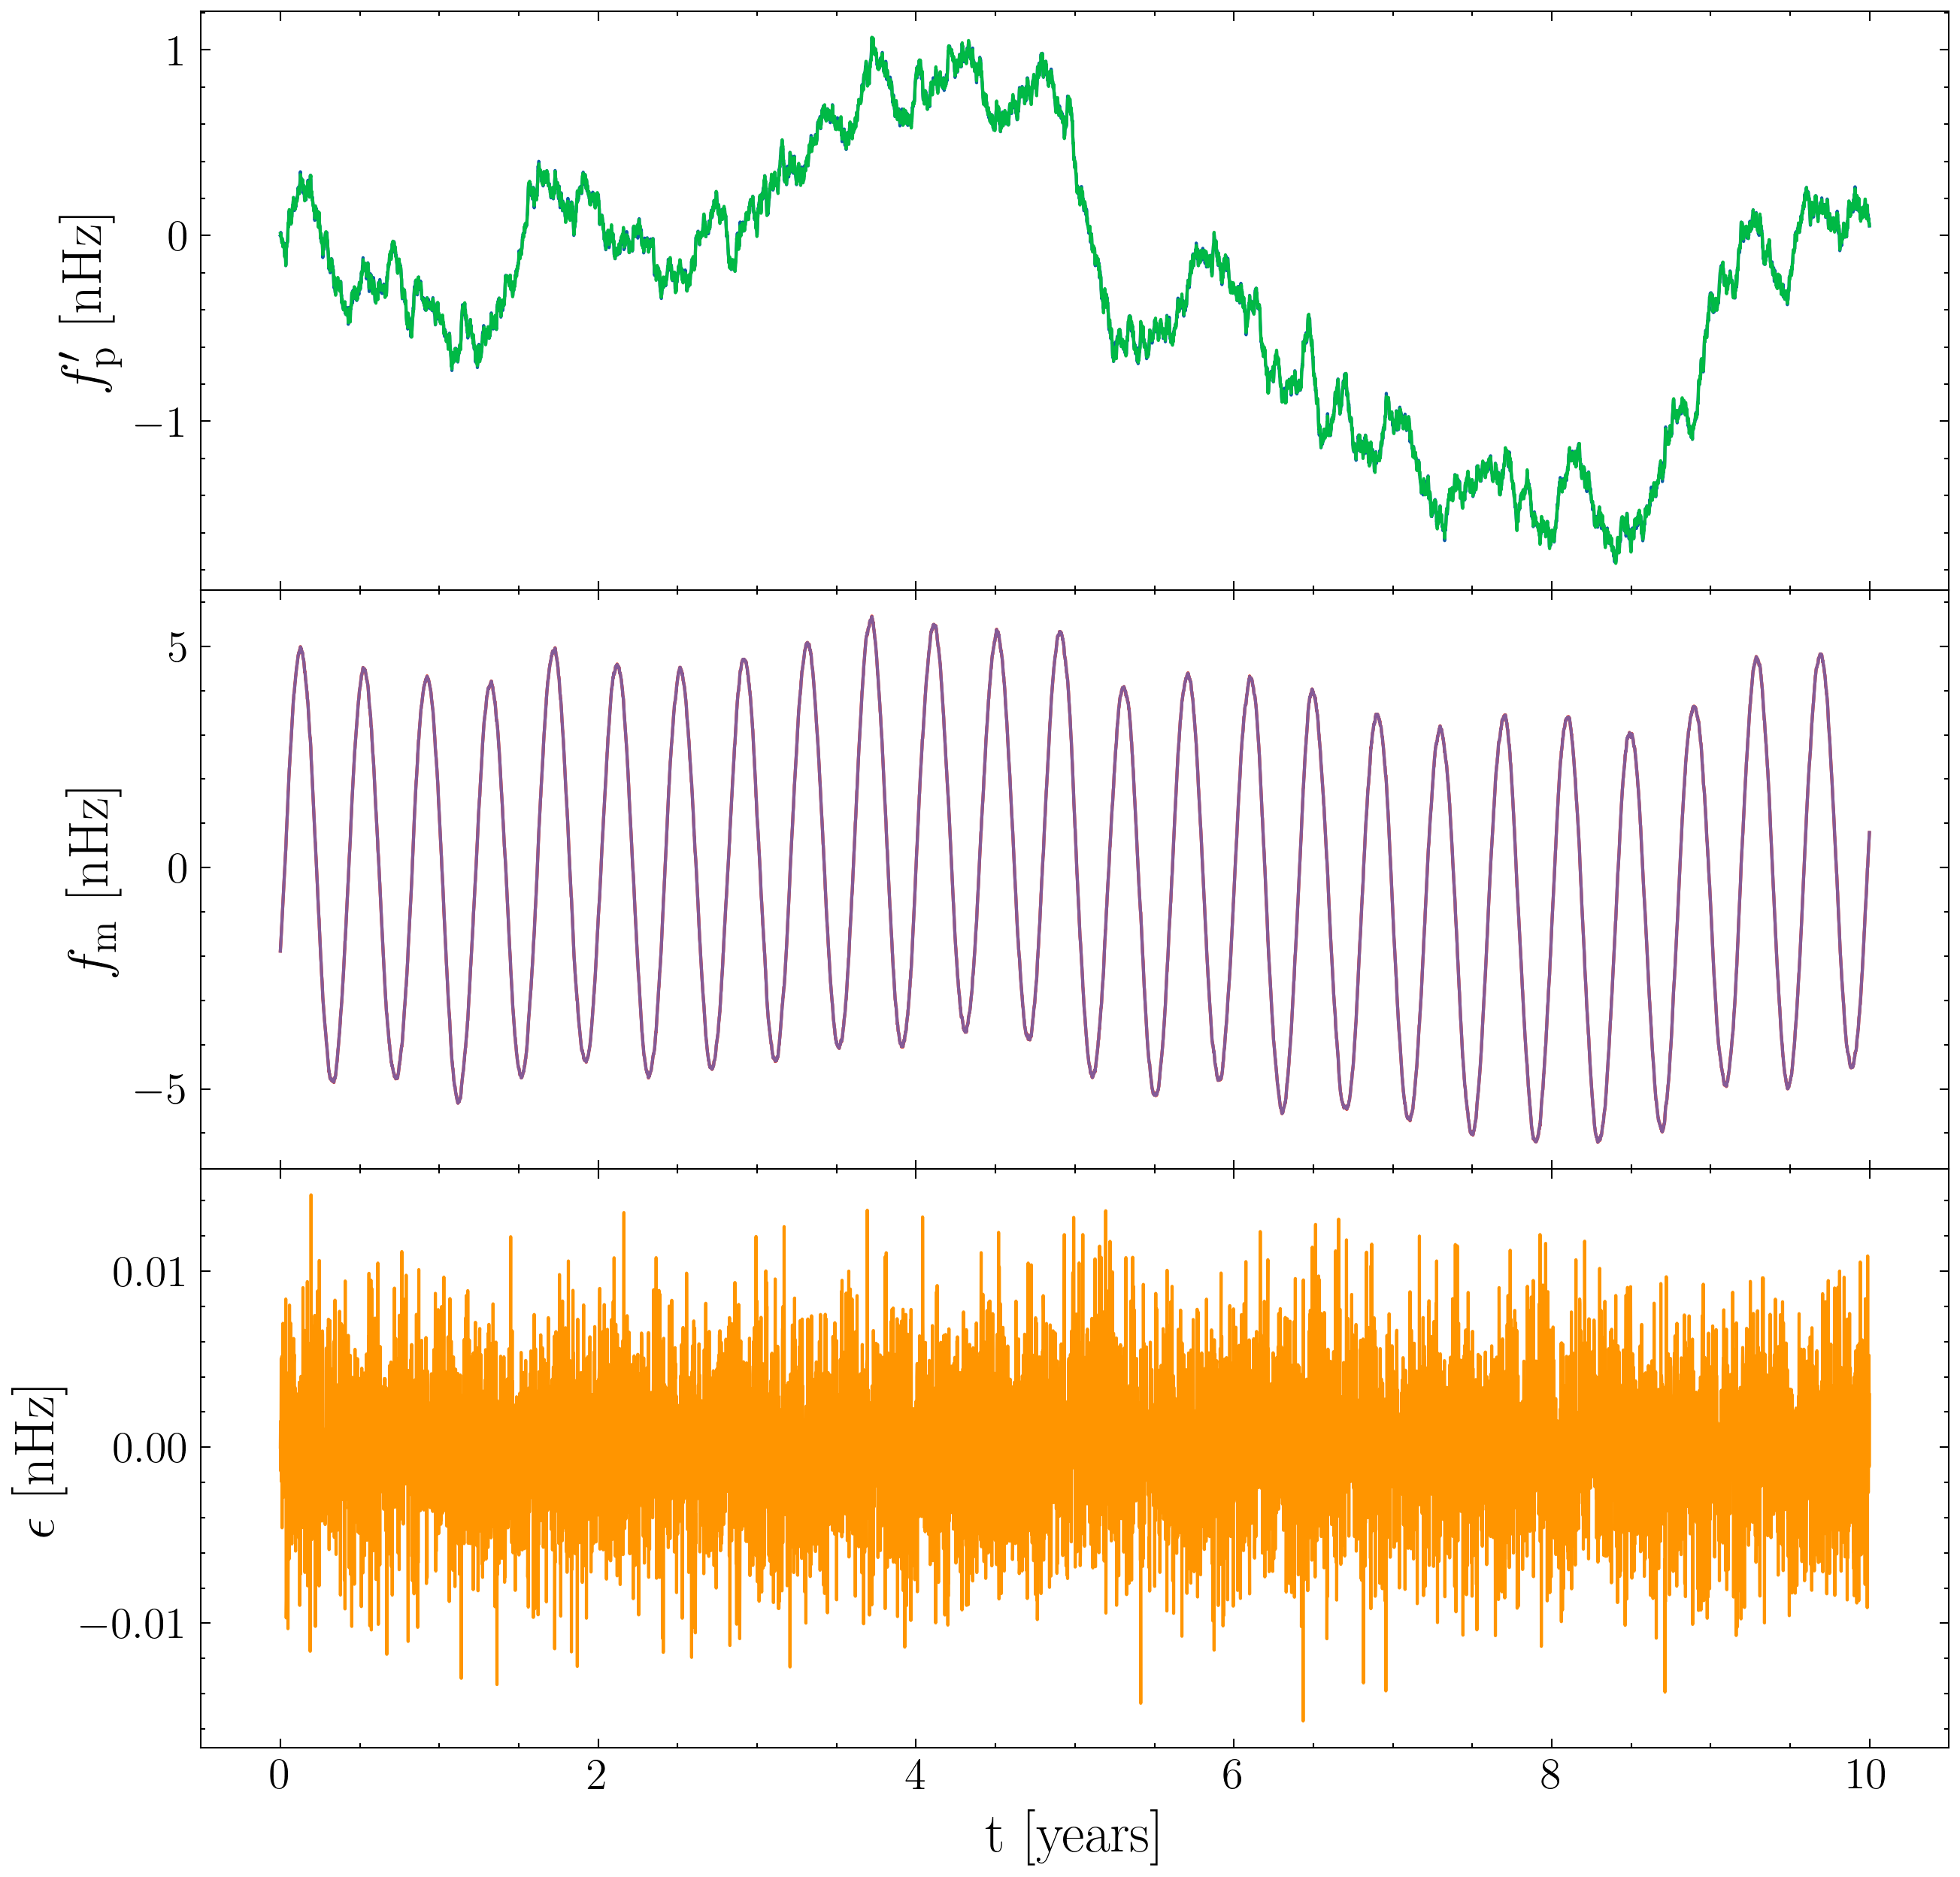
\includegraphics[width=\textwidth]{images/Kalman_example_true_params_single}
%		\caption{Kalman filter using correct estimate of the static parameters, $\hat{\boldsymbol{\theta}} = \boldsymbol{\theta}$ }
%		\label{fig:6MB_BFS}
%	\end{subfigure}  
%    \hfill
%	\begin{subfigure}[b]{0.49\textwidth}
%		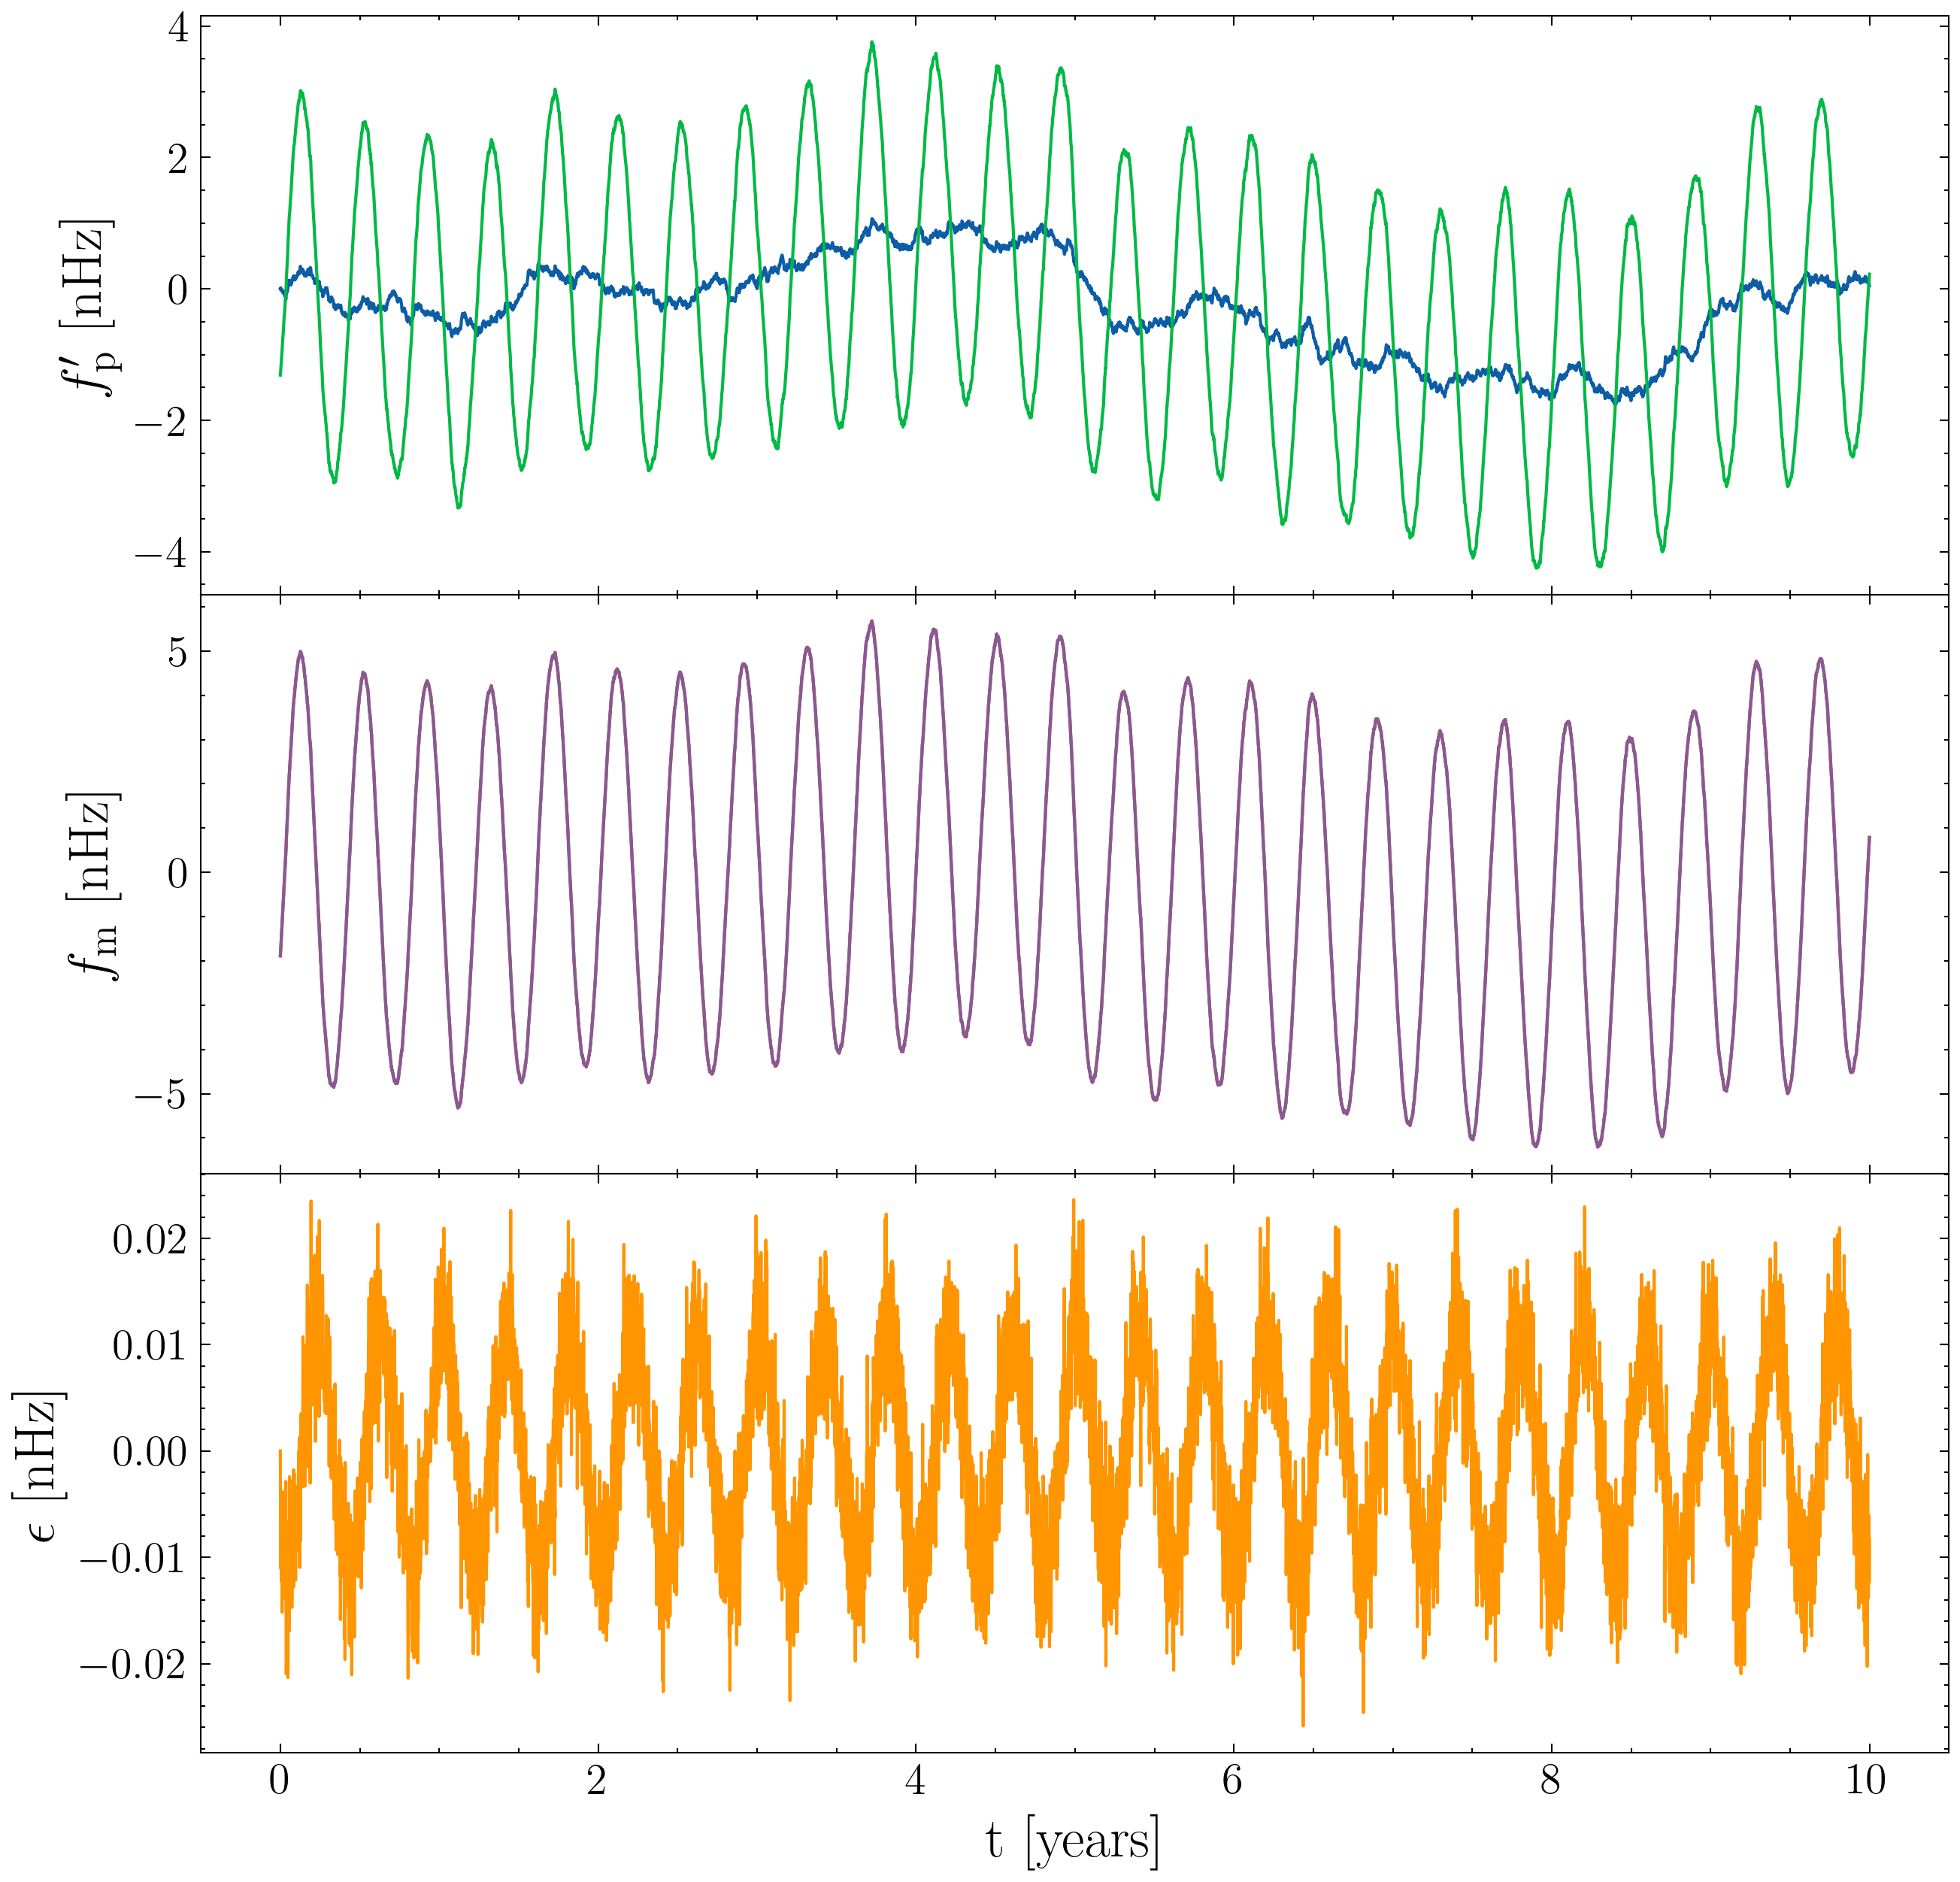
\includegraphics[width=\textwidth]{images/Kalman_example_wrong_params}
%		\caption{Kalman filter using incorrect estimate of the static parameters, $\hat{\boldsymbol{\theta}} \neq \boldsymbol{\theta}$}
%		\label{fig:25MB_bfs}
%	\end{subfigure}
%	\caption{
%		}
%	\label{fig:four figures}
%\end{figure*}


\begin{figure*}
	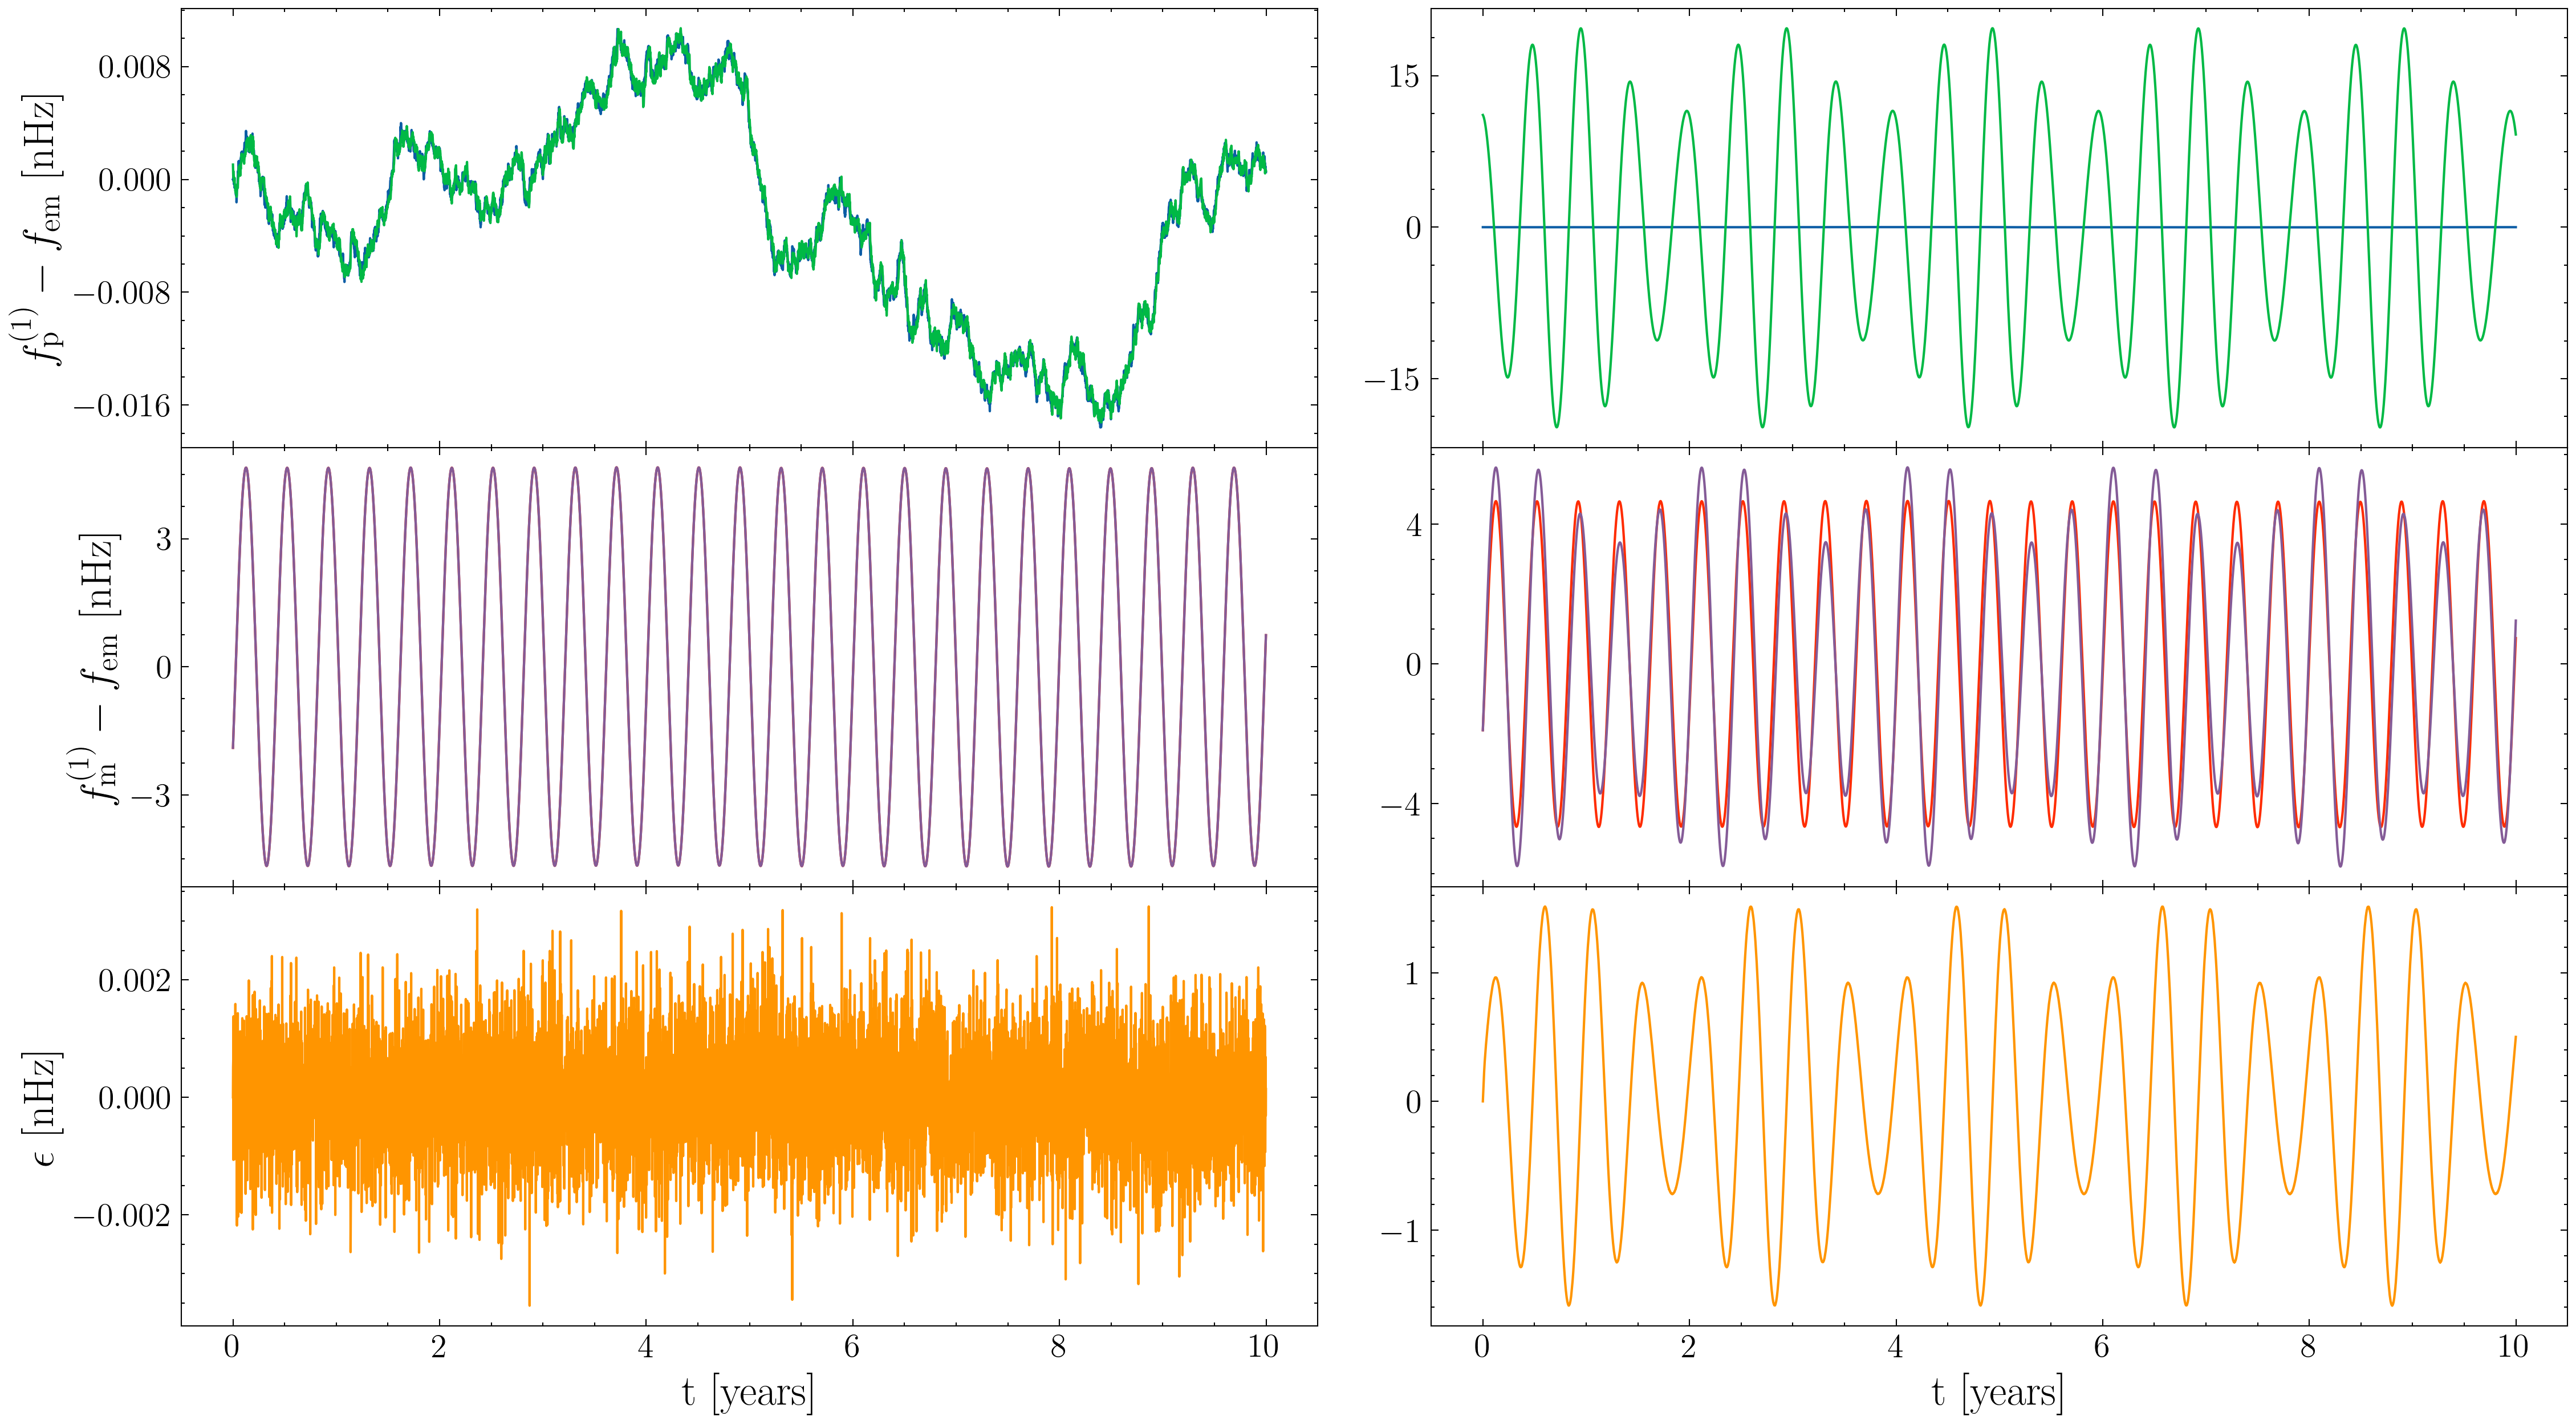
\includegraphics[width=\textwidth, height =0.5\textwidth]{images/Kalman_example_both}
	\caption{Sample output of the Kalman filter illustrating the accuracy of the reconstructed state sequence $f_{\rm p}^{(1)}(t)$ when the static parameters are correct (${\boldsymbol{\hat\theta}} = {\boldsymbol{\theta}}$, left column) and incorrect (${\boldsymbol{\hat\theta}} \neq {\boldsymbol{\theta}}$, right column). The top panels show the true pulsar state $f_{\rm p}^{(1)}(t) - f_{\rm em}^{(1)}(t)$ (blue curve) and the state estimated by the Kalman filter $\hat{f}_{\rm p}^{(1)}(t) - f_{\rm em}^{(1)}(t)$  (green curve). We subtract $f_{\rm em}^{(1)}(t)$ to better illustrate the stochastic wandering of the pulsar frequency. In the left column, the blue/green solutions overlap almost perfectly; in the right column, they do not. The middle panels show the true measured frequency $f_{\rm m}^{(1)}(t) - f_{\rm em}^{(1)}(t)$ (red curve) and the frequency estimated  by the Kalman filter $\hat{f}_{\rm m}^{(1)}(t) - f_{\rm em}^{(1)}(t)$ (magenta curve). Again we subtract $f_{\rm em}^{(1)}(t)$. In the left column the red/magenta solutions overlap almost perfectly; in the right column, they do not. The bottom panels show the residual or the innovation $\epsilon(t) =f_{\rm m}^{(1)}(t) - \hat{f}_{\rm m}^{(1)}(t)$. The results are shown for a single pulsar. In the right column $\Omega$ is displaced from its true value by 20\%.} 
	\label{fig:kalman_example}
\end{figure*}


The Kalman filter \citep{Kalman1} is a Gauss-Markov model used to algorithmically recover a temporal sequence of stochastically evolving  system state variables, $\boldsymbol{X}(t)$, which are not observed directly, given a temporal sequence of noisy measurements, $\boldsymbol{Y}(t)$. It finds common use in engineering applications and has been applied successfully in neutron star astrophysics \citep[e.g.][]{Myers2021MNRAS.502.3113M,Meyers2021,Melatos2023}. In this work we use the linear Kalman filter, which assumes a linear relation between $d{\boldsymbol{X}}/dt$ and ${\boldsymbol{X}}(t)$ (dynamics) and between ${\boldsymbol{Y}}(t)$ and ${\boldsymbol{X}}(t)$ (measurement), with ${\boldsymbol{X}}(t) = \{ f_{\rm p}^{(n)}(t) \}$ and ${\boldsymbol{Y}}(t) = \{ f_{\rm m}^{(n)}(t) \}$. Extension to non-linear problems is straightforward using either an extended Kalman filter \citep{zarchan2000fundamentals}, unscented Kalman filter \citep{882463van} or particle filter \citep{Simon10}. Equations \eqref{eq:measurement} and \eqref{eq:g_func} are non-linear in the static parameters (e.g.\ $d^{(n)}$), even though they are linear in ${\boldsymbol{X}}(t)$ and ${\boldsymbol{Y}}(t)$. Hence inferring the static parameters is a non-linear exercise, to be tackled separately after the linear Kalman filter operates on the data for a fixed set of static parameters. Inference of the static parameters in Equations \eqref{eq:measurement} and \eqref{eq:g_func} by nested sampling is discussed in Section \ref{sec:nested_sampling}. \newline 

Implementation of the linear Kalman filter for the PTA state-space model in Section 3.2, including the full set of Kalman recursion relations is presented in Appendix \ref{sec:kalman}. At each discrete timestep indexed by $ 1 \leq i  \leq M$, the Kalman filter returns an estimate of the state variables, $\hat{\boldsymbol{X}}_i = \hat{\boldsymbol{X}}(t_i)$, and the covariance of those estimates, ${\boldsymbol{P}}_i = \langle {\boldsymbol{\hat X}}_i {\boldsymbol{\hat X}}_i^{\rm T} \rangle$, where the superscript T denotes the matrix transpose. The filter tracks the error in its predictions of $\boldsymbol{X}_i$ by converting ${\boldsymbol{\hat X}}_i$ into predicted measurements ${\boldsymbol{\hat Y}}_i$ via Equations \eqref{eq:measurement} and \eqref{eq:g_func} and comparing with the actual, noisy measurements ${\boldsymbol{\hat Y}}_i$. This defines a residual $\boldsymbol{\epsilon}_i = \boldsymbol{Y}_i  - \hat{\boldsymbol{Y}}_i$, which is sometimes termed the innovation. The Kalman filter also calculates the uncertainty in $\boldsymbol{\epsilon}_i$ via the innovation covariance $\boldsymbol{S}_i = \langle \boldsymbol{\epsilon}_i \boldsymbol{\epsilon}_i^{T} \rangle$. The innovation and the innovation covariance are then used to correct the state estimate ${\boldsymbol{\hat X}}_i$ according to Equation \eqref{eq:kalmangainupdate}. For a fixed set of static parameters, the Kalman filter returns an estimate of the state sequence ${\boldsymbol {\hat X}}_1, \dots , {\boldsymbol{\hat X}}_M$ which minimizes the mean square error. We explain how to use this intermediate output to infer the optimal values of the static parameters ${\boldsymbol{\theta}}$ in Section \ref{sec:nested_sampling} \newline 


The Gaussian log-likelihood of obtaining ${\boldsymbol{Y}}_i$ given ${\boldsymbol{\hat X}}_i$ can  then be calculated at each timestep from the Kalman filter output according to
\begin{eqnarray}
	\log \mathcal{L}_i =  -\frac{1}{2} \left (N \log 2 \pi + \log  \left | \boldsymbol{S}_i \right | + \boldsymbol{\epsilon}_i^{\intercal} \boldsymbol{S}_i^{-1}  \boldsymbol{\epsilon}_i \right ) \ .
\end{eqnarray}
The total log-likelihood for the entire sequence is
\begin{eqnarray}
	\log \mathcal{L} =  \sum_{i=1}^{M} \log \mathcal{L}_i \ . \label{eq:likelihood}
\end{eqnarray}
Given ${\boldsymbol{Y}}_1, \dots, {\boldsymbol{Y}}_M$, $\mathcal{L}$ is a function of the estimates ${\boldsymbol{\hat \theta}}$ of the static parameters passed to the Kalman filter, i.e. $\mathcal{L}$ = $\mathcal{L}(\boldsymbol{Y} | \boldsymbol{\hat \theta})$. Similarly the estimates of the state and measurement variables, $\hat{\boldsymbol{X}}$ and $\hat{\boldsymbol{Y}}$, are functions of $\boldsymbol{\hat \theta}$. If $\boldsymbol{\hat{\theta}}$ is close to the true underlying parameters $\boldsymbol{\theta}$, then the errors in $\hat{\boldsymbol{X}}$ and $\hat{\boldsymbol{Y}}$ are minimized and $\mathcal{L}$ is maximised. This is illustrated with synthetic data in Figure \ref{fig:kalman_example}. In the left column, a time series of $f_{\rm m}^{(1)}(t)$ including Gaussian noise (middle panel, red curve) is generated from Equations \eqref{eq:spinevol}-- \eqref{eq:xieqn}, \eqref{eq:measurement}, and \eqref{eq:g_func} for a single pulsar and fed into the Kalman filter along with the true static parameters ${\boldsymbol{\hat \theta}} = {\boldsymbol{\theta}}$. The Kalman filter recovers the evolution of $f_{\rm p}^{(1)}(t)$ with high fidelity; the estimate of $\hat{f}_{\rm p}^{(1)}(t)$ (left top panel, blue curve) overlaps almost perfectly with the true $f_{\rm p}^{(1)}(t)$ (left top panel, green curve). The predicted state $\hat{f}_{\rm p}^{(1)}(t)$ is converted  into a predicted measurement $\hat{f}_{\rm m}^{(1)}(t)$ (middle panel, magenta curve), which again overlaps almost perfectly with the true measurement. The residuals $\epsilon(t)$ between the true and predicted measurements are small ($\lesssim 0.1\%$) and normally distributed (left bottom panel). By contrast, in the right column, the exercise is repeated while passing slightly incorrect static parameters (${\boldsymbol{\hat\theta}} \neq {\boldsymbol{\theta}}$) to the Kalman filter, where $\Omega$ is displaced from its true value by $20 \%$. In this case the Kalman filter fails to track $f_{\rm p}^{(1)}(t)$ accurately, as the discrepancy between the blue and green curves in the top panel of the right-hand column indicates. It similarly fails to predict $f_{\rm m}^{(1)}(t)$ accurately, as shown by the discrepancy between the red and magenta curves in the middle panel, and the residuals are no longer distributed normally (right bottom panel).


%n Figure ; given a timeseries of the measured pulsar frequency the Kalman filter is able to recover the evolution of the hidden state with high fidelity. The residuals correspond to random noise and are normally distributed. Conversely, if $\boldsymbol{\hat{\theta}}$ is not close to the true parameters then the filter is unable to recover the state evolution. This is demonstrated in Figure \ref{fig:25MB_bfs} where the Kalman filter was run with $\boldsymbol{\hat{\theta}}$ slightly perturbed away from the true values. In this case the filter cannot track the state variable accurately and the residuals are no longer Gaussian.


\subsection{Nested sampling}\label{sec:nested_sampling}
We can use the likelihood returned by the Kalman filter, Equation \eqref{eq:likelihood}, in conjunction with likelihood-based inference methods to estimate the posterior distribution of $\boldsymbol{\theta}$ by Bayes' Rule,
\begin{equation}
	p(\boldsymbol{\theta} | \boldsymbol{Y}) = \frac{\mathcal{L}(\boldsymbol{Y} | \boldsymbol{\theta}) \pi(\boldsymbol{\theta})}{\mathcal{Z}} \ ,
\end{equation}
where $\pi(\boldsymbol{\theta})$ is the prior distribution on $\boldsymbol{\theta}$ and $\mathcal{Z}$ is the marginalised likelihood, or evidence
\begin{equation}
	\mathcal{Z} = \int d \boldsymbol{\theta} \mathcal{L}(\boldsymbol{Y} | \boldsymbol{\theta})  \pi(\boldsymbol{\theta})  \ . \label{eq:model_evidence}
\end{equation}
 We estimate the posterior distribution and the model evidence through nested sampling \citep{Skilling} in this paper. Nested sampling evaluates marginalised likelihood integrals, of the form given by Equation \eqref{eq:model_evidence}. It also approximates the posterior by returning samples from $p(\boldsymbol{\theta} | \boldsymbol{Y})$. It does so by drawing a set of $n_{\rm live}$ live points from $\pi(\boldsymbol{\theta})$ and iteratively replacing the live point with the lowest likelihood with a new live point drawn from $\pi(\boldsymbol{\theta})$, where the new live point is required to have a higher likelihood than the discarded point. The primary advantage of nested sampling is its ability to compute $\mathcal{Z}$, on which model selection relies. Nested sampling is also computationally efficient and can handle multi-modal problems \citep{Ashton2022}. For these reasons, it has enjoyed widespread adoption in the physical sciences, particularly within the cosmological community \citep{Mukherjee2006,Feroz2008,Handley2015}, neutron star astrophysics \citep{Myers2021MNRAS.502.3113M,Meyers2021,Melatos2023}, particle physics \citep{proceedings2019033014} and materials science \citep{2009arXiv0906materials}. For a review of nested sampling we refer the reader to \cite{Buchner2021} and \cite{Ashton2022}. Multiple nested sampling algorithms and computational libraries exist. \citep[e.g.][]{Feroz2008,Feroz2009,Handley2015,dynesty2020,UltraNest2021}. In gravitational wave research it is common to use the \texttt{dynesty} sampler \citep{dynesty2020} via the \texttt{Bilby} \citep{bilby.507.2037A} front-end library. We follow this precedent and use \texttt{Bilby} for all nested sampling Bayesian inference in this work. \newline 
 
The primary tunable parameter in nested sampling is $n_{\rm live}$. More live points assists with large parameter spaces and multi-modal problems, whilst the uncertainties in the evidence and the posterior scale as $\mathcal{O}\left(n_{\rm live}^{-1/2}\right)$. However the computational runtime scales as $\mathcal{O}(n_{\rm live})$. \cite{Ashton2022} offered a rule-of-thumb trade-off, where the minimum number of live points should be greater than the number of static parameters. Informal empirical tests conducted as part of this paper support the trade-off suggested by \cite{Ashton2022}; we find typically that the true ${\boldsymbol{\theta}}$ is contained within the 90\% credible interval of the one-dimensional marginalised posteriors of ${\boldsymbol{\hat{\theta}}}$ for $n_{\rm live} > 7 + 5N$ with $N \leq 50$. Unless stated otherwise we take $n_{\rm live} = 1000$ for all results presented in this work. \newline 

%See https://arxiv.org/pdf/2102.12478.pdf for a good NS explanation

\subsection{Model selection}\label{sec:model_selection}
The evidence integral $\mathcal{Z}$ returned by nested sampling is the probability of the data $\boldsymbol{Y}$ given a model $\mathcal{M}_i$. We compare competing models via a Bayes factor,
\begin{equation}
	\beta = \frac{\mathcal{Z}(\boldsymbol{Y} | \mathcal{M}_1)}{\mathcal{Z}(\boldsymbol{Y} | \mathcal{M}_0)} \ . \label{eq:bayes}
\end{equation}
Throughout this work we take $\mathcal{M}_1$ to be the state-space model that includes the presence of a GW. $\mathcal{M}_0$ is the null model, which assumes no GW exists in the data, and is equivalent to setting $g^{(n)}(t)=1$ in Equations \eqref{eq:g_func} and \eqref{eq:g_func_trig}. The Bayes factors we quote in this work therefore quantify whether the data supports evidence for a GW signal compared to there being no GW signal present.


\subsection{Summary of workflow}\label{sec:methodsummary}
For the reader's convenience we now summarise the workflow for a representative PTA analysis using the Kalman filter and nested sampler for parameter estimation and model selection:
\begin{enumerate}[leftmargin=2em]
	\item Specify a PTA composed of $N$ pulsars 
	\item Obtain $N$ data inputs $f_{\rm m}^{(n)}(t)$, collectively labelled $\boldsymbol{Y}$
	\item Specify a state-space model $\mathcal{M}$, with static parameters $\boldsymbol{\theta}$. 
	\item Specify prior distribution $\pi(\boldsymbol{\theta})$
	 \item Sample $n_{\rm live}$ points from $\pi(\boldsymbol{\theta})$ 
	 \item For each live point:
\begin{enumerate}[leftmargin=2em]
	\item Pass the sample $\boldsymbol{\theta}_{\rm sample}$ to the Kalman filter.
	\item Iterate over the input data using the Kalman filter and obtain a single $\log \mathcal{L}$ value, Equation \eqref{eq:likelihood}
\end{enumerate}
	\item Remove the live point with the lowest likelihood value, $\log \mathcal{L}_{\rm lowest}$
	\item Sample a new live point from $\pi(\boldsymbol{\theta})$, subject to the requirement that the new likelihood obeys $\mathcal{L}_{\rm new}$ > $\mathcal{L}_{\rm lowest}$, where  $\log \mathcal{L}_{\rm new}$ is calculated via steps (vi)(a) -- (vi)(b).
	\item Update $p\left(\boldsymbol{\theta}|\boldsymbol{Y}\right)$ and $\mathcal{Z}$ with nested sampler
	\item Repeat steps (vii) - (ix) until convergence criteria are satisfied.
\end{enumerate}
In order to compute $\beta$ the above workflow is repeated for a different $\mathcal{M}$. The resulting $\mathcal{Z}$ values can then be compared. We remind the reader that the above workflow differs from a realistic PTA analysis in one important respect, namely that the data are input as frequency time series $f_{\rm m}^{(n)}(t)$ instead of pulse TOAs. The generalization to TOAs is subtle and will be tackled in a forthcoming paper.

\section{Validation with synthetic data} \label{sec:testing}
In this section we outline how synthetic data are generated in order to validate the analysis scheme in Section \ref{sec:detect}. Synthetic data enable validation to occur systematically and under controlled conditions. In Section \ref{sec:synt_pta} we describe how to construct a representative synthetic PTA, and how to set astronomically reasonable values for the static pulsar parameters $\boldsymbol{\theta}_{\rm psr}$. In Section \ref{sec:gendata} we demonstrate how to solve Equations \eqref{eq:spinevol} -- \eqref{eq:frequency_evolution}, and \eqref{eq:measurement} -- \eqref{eq:g_func} for the synthetic PTA so as to generate noisy, frequency time series $f_{\rm m}^{(n)}(t)$. 

\subsection{Constructing a synthetic PTA}\label{sec:synt_pta}
\begin{figure}
	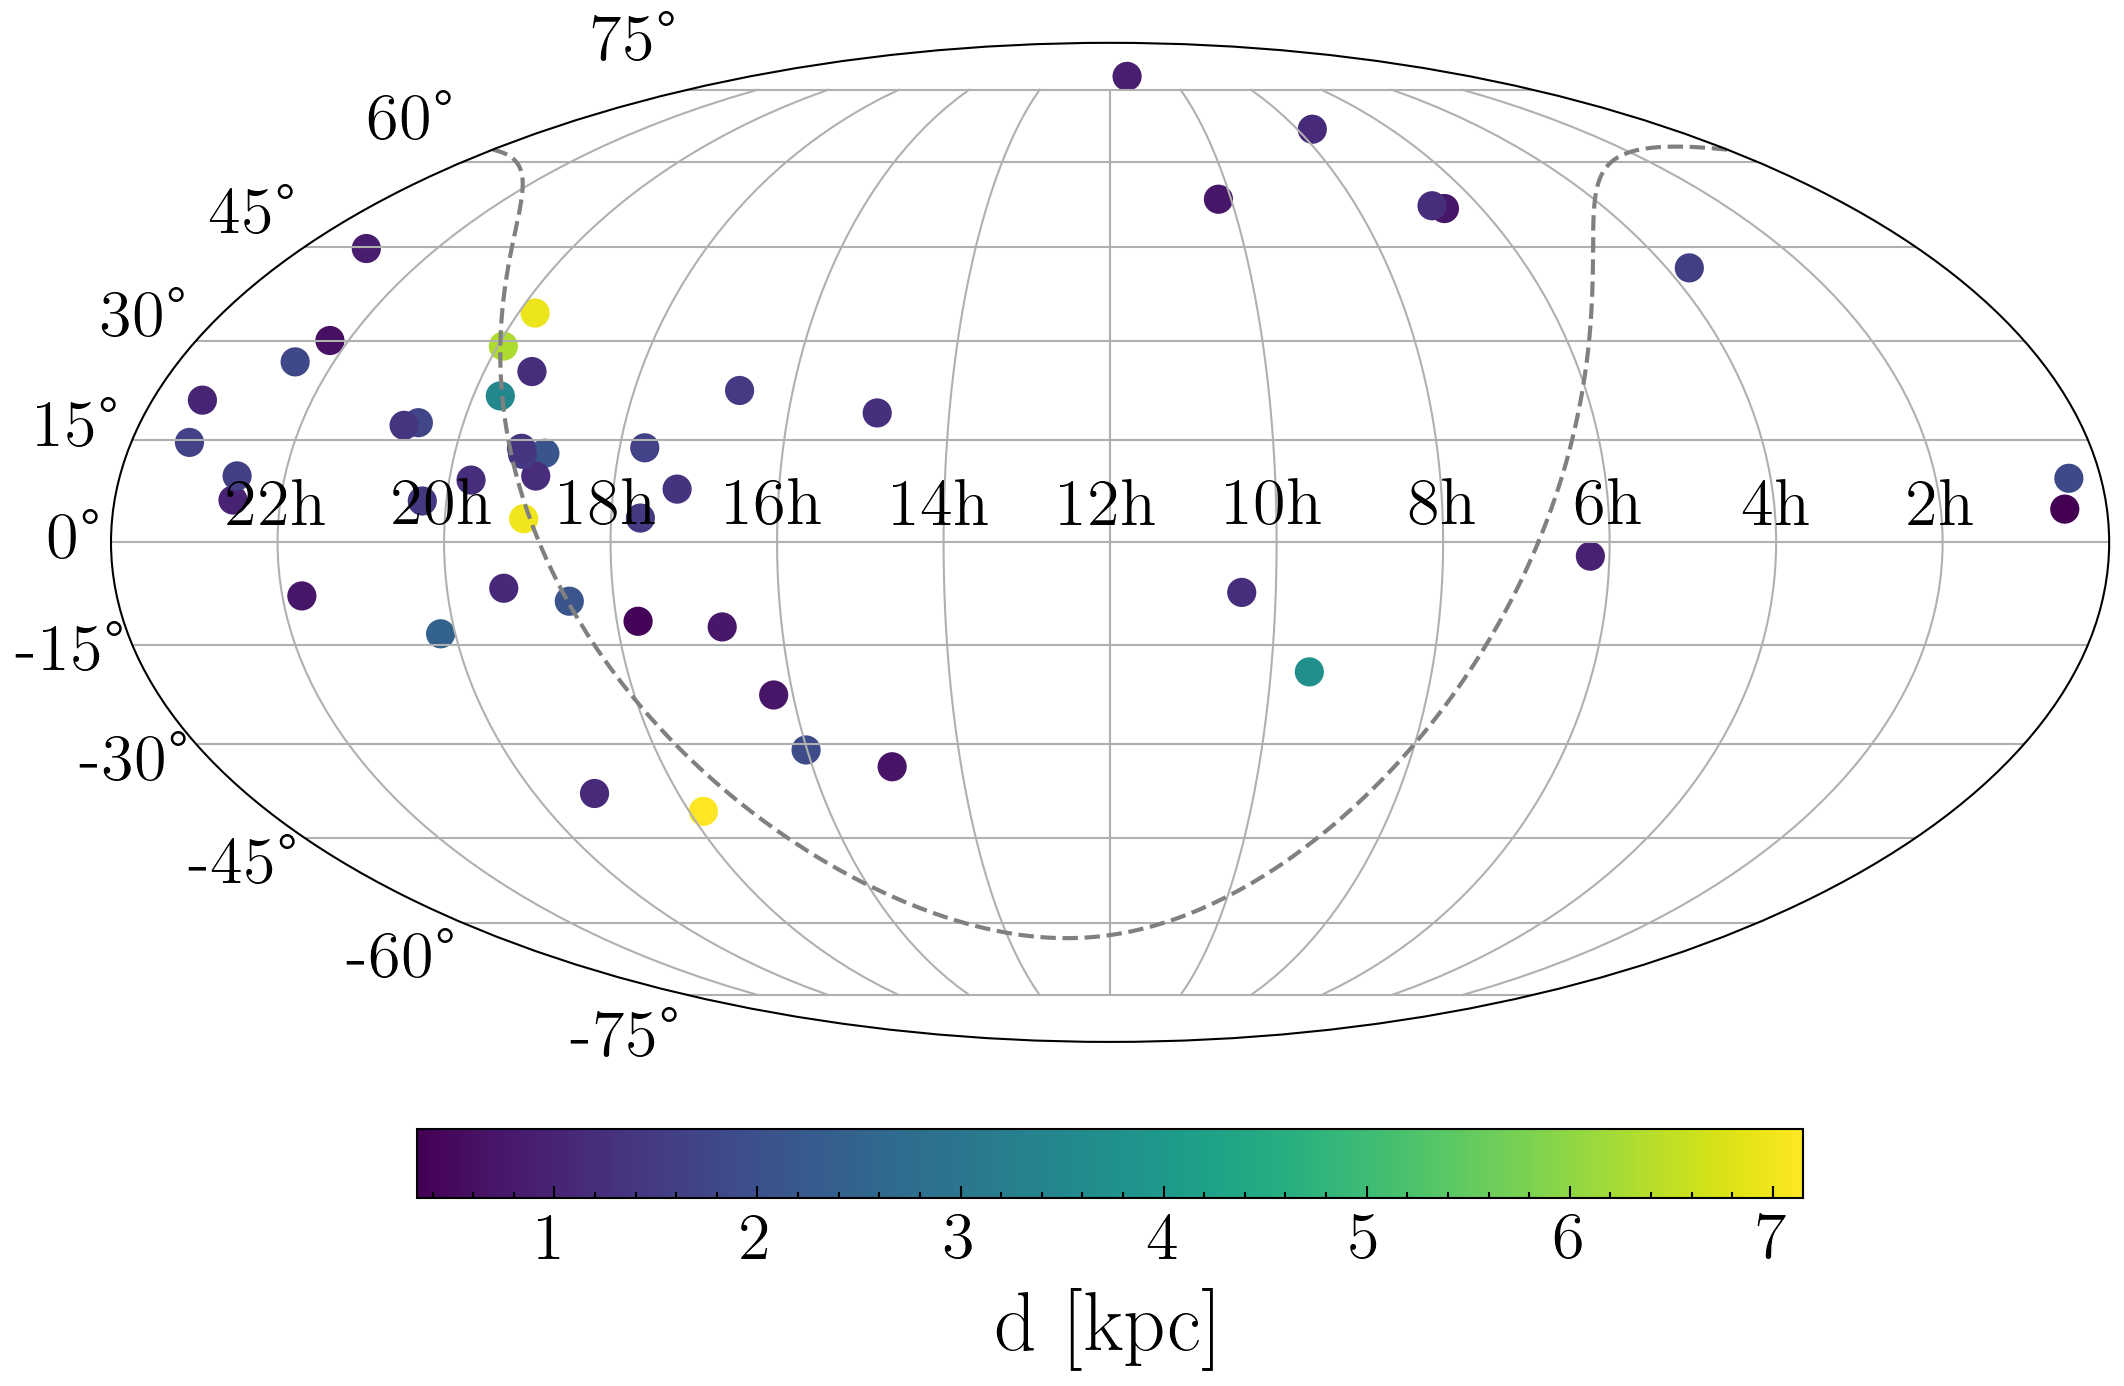
\includegraphics[width=\columnwidth]{images/pulsar_distribution}
	\caption{Spatial distribution in Galactic coordinates of 47 pulsars from the 12.5 year NANOGrav data release that make up the synthetic PTA used in this work. The pulsar distances relative to the observer are also indicated, with a distance $\leq 2 \, {\rm kpc}$ for $38$ pulsars. The grey dashed curve denotes the Galactic plane.}
	\label{fig:pulsar_distrib}
\end{figure}
We consider, by way of illustration, a synthetic PTA composed of the 47 pulsars in the 12.5 year NANOGrav dataset \citep{2020ApJ...905L..34A}. The NANOGrav pulsars are chosen arbitrarily as being representative of a typical PTA; the analysis below extends unchanged to any other PTA. \newline 

For each pulsar we adopt fiducial values for ${\boldsymbol{q}}^{(n)}$, $d^{(n)}$, $f_{\rm em}^{(n)}(t_1)$, and $\dot{f}_{\rm em}(t_1)$, with the latter two quantities evaluated at the Solar System barycenter. A table of fiducial values is presented in Appendix \ref{appendix_fiducial} for the sake of reproducibility. The sky positions and colour-coded distances of the pulsars are displayed in Figure \ref{fig:pulsar_distrib}. The pulsar parameters are acquired via the Australia Telescope National Facility (ATNF) pulsar catalogue \citep{Manchester2005} using the \texttt{psrqpy} package \citep{psrqpy}. \newline 

The remaining static pulsar parameters are $\gamma^{(n)}$ and $\sigma^{(n)}$, for which no direct measurements exist. The ratio $\sigma^{(n)} / [\gamma^{(n)}]^{1/2}$ sets the typical root mean square fluctuations in $f_p^{(n)}(t)$, as discussed in Section \ref{sec:psr_frequency}, and the mean reversion timescale typically satisfies $[\gamma^{(n)}]^{-1} \gg T_{\rm obs}$ \citep{Price2012,Myers2021MNRAS.502.3113M,Meyers2021,Vargas}. In this paper, for the sake of simplicity in the absence of independent measurements, we fix $\gamma^{(n)} = 10^{-13}$ s$^{-1}$ for all $n$. We follow two complementary approaches in order to  set physically reasonable values for $\sigma^{(n)}$. The first approach relies on the empirical timing noise model from \cite{Shannon2010ApJ...725.1607S} which gives the standard deviation of the pulsar TOAs, $\sigma_{\rm TOA}^{(n)}$, empirically as
\begin{align}
	\ln \left(\frac{\sigma_{\rm TOA}^{(n)}}{\mu s} \right)=& \ln \alpha_1 +  \alpha_2 \ln f_{\rm p}^{(n)} + \alpha_3 \ln \left(\frac{\dot{f}_{\rm p}^{(n)}}{10^{-15} \text{s}^{-2}} \right) \nonumber \\ 
	&+ \alpha_4 \ln \left( \frac{T_{\rm cad}}{ 1 \text{ year}} \right) \ , \label{eq:sigmap}
\end{align}
where $T_{\rm cad}$ is the cadence of the timing observations. For MSPs the best fit parameters are $\ln \alpha_1 = -20 \pm 20$, $\alpha_2 = 1 \pm 2 $, $\alpha_3 = 2 \pm 1$, $\alpha_4 = 2.4 \pm 0.6$ ($\pm 2\sigma$ confidence limits). The uncertainties are broad; for the purpose of generating astrophysically representative synthetic data we straightforwardly adopt the central values in this paper. Throughout this work we assume for simplicity that all pulsars are observed with a weekly cadence, $T_{\rm cad} = 1 \,{\rm week}$. In order to relate Equation \eqref{eq:sigmap} to $\sigma^{(n)}$ in Equation \eqref{eq:spinevol}, we equate $\sigma^{(n)}$ to the root mean square TOA noise accumulated over one week, obtaining
\begin{eqnarray}
	\sigma^{(n)} \approx \sigma_{\rm TOA}^{(n)} f_{\rm p}^{(n)} {T_{\rm cad}}^{-3/2} \ . \label{eq:sigmap_f}
\end{eqnarray}
For the synthetic NANOGrav PTA depicted in Figure \ref{fig:pulsar_distrib}, the median $\sigma^{(n)}$ calculated in this way is $\sigma^{(n)} = 5.51 \times 10^{-24} $ s$^{-3/2}$, with $\min [ \sigma^{(n)} ] = 1.67 \times 10^{-26}$s$^{-3/2}$ for PSR J0645+5158 and $\max [ \sigma^{(n)} ] = 2.56 \times 10^{-19}$ s$^{-3/2}$ for PSR J1939+2134 \newline 

As a cross-check, we estimate $\sigma^{(n)}$ by solving Equation \eqref{eq:spinevol} numerically using the \texttt{baboo} package \footnote{\url{https://github.com/meyers-academic/baboo}}, generating a synthetic phase solution,
\begin{eqnarray}
	\varphi^{(n)}(t) = \int_0^t dt' f^{(n)}_{\rm p}(t') \ ,
\end{eqnarray}
and adjusting $\sigma^{(n)}$ iteratively to generate phase residuals which qualitatively (i.e.\ visually) resemble empirical phase residuals measured from real pulsars; see Section 2 in \cite{Vargas} for a successful example of this approach. We obtain empirical phase residuals from the NANOGrav 12.5 year wideband timing dataset \citep{pennucci_timothy_t_2020_4312887,nanogravwideband}. A visual cross-check is sufficient for the purposes of this paper, where we seek broadly representative values for $\sigma^{(n)}$. In an analysis involving real PTA data, $\sigma^{(n)}$ would be estimated from the data jointly with the other static parameters in ${\boldsymbol{\theta}}$. In Figure \ref{fig:qualitative_compare} we compare the synthetic and empirical residuals for PSR J1939+2134, one of the 47 NANOGrav pulsars plotted in Figure \ref{fig:pulsar_distrib}. We see that the synthetic and empirical residuals are qualitatively similar. For this pulsar the synthetic residuals are generated using $\sigma^{(n)} = 2 \times 10^{-27}$ s$^{-3/2}$ which is $\ll$ than the central value $\sigma^{(n)} = 2.56 \times 10^{-19}$ s$^{-3/2}$ inferred from Equations \eqref{eq:sigmap} and \eqref{eq:sigmap_f}, but is consistent with the wide ranges on $\alpha_1$, $\dots$, $\alpha_4$, e.g.\ $\ln \alpha_1 = -38$ implies $\sigma^{(n)}= 3.90 \times 10^{-27}$ for PSR J1939$+$2134.

%This highlights how given the large uncertainties on the parameters of Equation \eqref{eq:sigmap} using the best fit values may be less appropriate for certain pulsars. If we set $\ln \alpha_1 = -38$ in Equation \eqref{eq:sigmap}, close to its lower limit, then the estimated $\sigma^{(n)}$ for  PSR J1939+2134 is $\sigma^{(n)} =3.90 \times 10^{-27}$ which is in much better agreement with the value inferred from the residuals comparison method.





\begin{figure}
	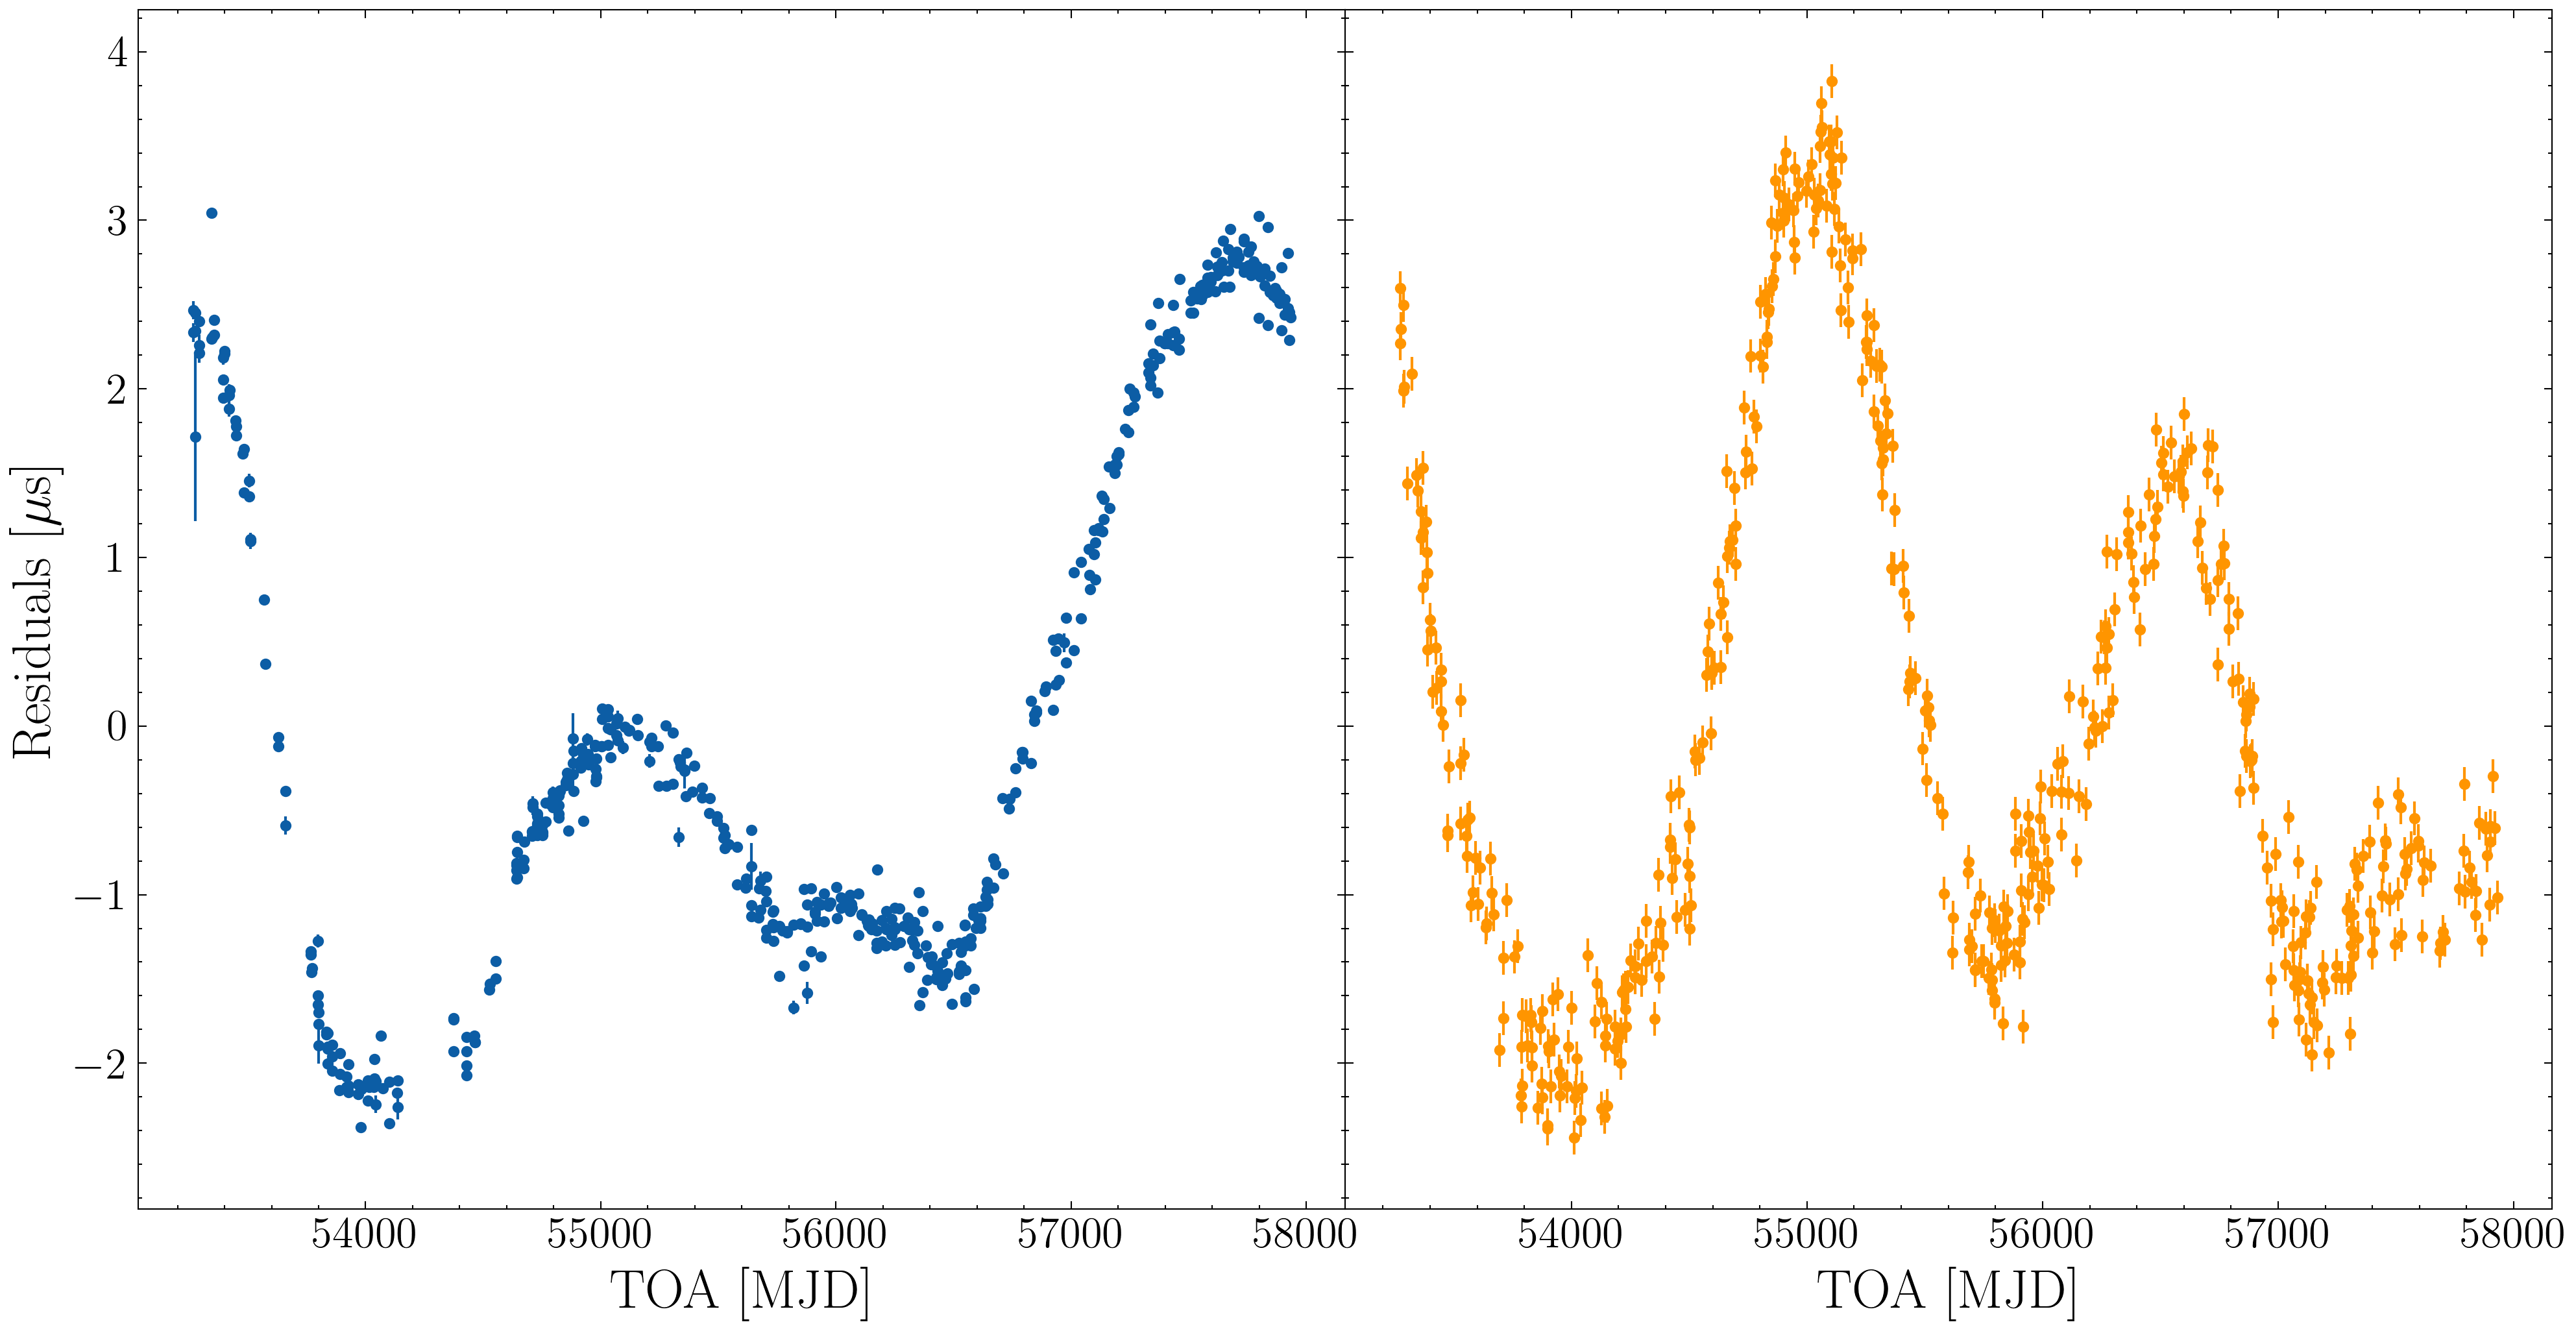
\includegraphics[width=\columnwidth]{images/example_residuals_plot2}
	\caption{Actual (left panel, blue points) and synthetic (right panel, orange points) phase residuals for NANOGrav millisecond pulsar PSR J1939+2134. The actual residuals are sourced from the NANOGrav 12.5 year wideband timing dataset \citep{pennucci_timothy_t_2020_4312887,nanogravwideband}. The synthetic residuals are generated by numerically solving Equation \eqref{eq:spinevol} with $\gamma^{(n)} = 10^{-13}$ and $\sigma^{(n)} = 2\times 10^{-27}$ s$^{-3/2}$. The error bars indicate the uncertainty in the phase residuals and are generated by propagating the uncertainty in the TOAs through {\sc tempo2}. We set the TOA uncertainty to be a constant, $0.1 \mu$s. The blue and orange residuals are qualitatively similar by inspection. Similar results are obtained for the other 46 pulsars in the synthetic PTA in Section \ref{sec:synt_pta} by tuning the value of $\sigma^{(n)}$.}
	\label{fig:qualitative_compare}
\end{figure}
\subsection{Generating a synthetic sequence of pulse frequencies}\label{sec:gendata}
We generate $N$ synthetic noisy time series of the measured pulse frequency $f_{\rm m}^{(n)}(t)$, one for each pulsar $1\leq n \leq N$, as follows:
\begin{enumerate}[leftmargin=2em]
	\item Integrate Equations \eqref{eq:spinevol}--\eqref{eq:xieqn} numerically for the synthetic PTA described in Section \ref{sec:synt_pta}, to obtain random realizations of $f_{\rm p}^{(n)}(t)$ for $1\leq n \leq N$.
	\item Map from $f_{\rm p}^{(n)}(t)$ to $f_{\rm m}^{(n)}(t)$ via Equations \eqref{eq:measurement} and \eqref{eq:g_func}.
\end{enumerate}
Equations \eqref{eq:spinevol}--\eqref{eq:xieqn} are solved by a Runge-Kutta It$\hat{\text{o}}$ integrator implemented in the \texttt{sdeint} python package \footnote{\url{https://github.com/mattja/sdeint}}. The static pulsar parameters  $\boldsymbol{\theta}_{\rm psr}$ are completely specified for the synthetic PTA outlined in Section \ref{sec:synt_pta}. For this work we consider all pulsars to be observed for $T_{\rm obs} =10$ years, uniformly sampled with a weekly cadence. \newline 


The measurement noise covariance as defined in Equation \eqref{eq:vareps} can be approximately related to the uncertainty in the pulse TOA, $\sigma_{\rm TOA}$, through
\begin{equation}
	\sigma_{\rm m} \approx \sigma_{\rm TOA} f_{\rm p}^{(n)}  \ {T_{\rm cad}}^{-1} \ . \label{eq:sigma_m_eqn}
\end{equation}
Although Equations \eqref{eq:sigmap_f} and \eqref{eq:sigma_m_eqn} superficially resemble one another, they are distinct. Equation \eqref{eq:sigmap_f} deals with the timing noise intrinsic to the pulsar due to rotational irregularities, whereas Equation \eqref{eq:sigma_m_eqn} handles the detector measurement noise. For a millisecond pulsar with $f_{\rm p}^{(n)} \sim 100$ Hz observed with a weekly cadence and $\sigma_{\rm TOA} \sim 1 \mu$s, Equation \eqref{eq:sigma_m_eqn} implies $\sigma_{\rm m} \sim 10^{-10}$ Hz. The most accurately timed pulsars have $\sigma_{\rm TOA} \sim 10 $ ns and $\sigma_{\rm m} \sim 10^{-12}$ Hz. Throughout this paper we fix $\sigma_{\rm m} = 10^{-11}$ Hz and take it as known \textit{a priori} rather than a parameter to be inferred for the sake of simplicity; this assumption can be relaxed easily when analysing real data. Whilst $\sigma_{\rm m}$ is the same for every pulsar, $f_{\rm m} ^{(n)}(t)$ is constructed from a different random realisation of $\varepsilon^{(n)}(t)$ for each pulsar. \newline 

Finite precision arithmetic leads to numerical errors when solving Equations \eqref{eq:spinevol}--\eqref{eq:xieqn} $ \text{in  the regime } |\sigma^{(n)} \Delta B_t | \ll f_{\rm p}^{(n)}$ relevant to PTAs, where $\Delta B_t$ labels an increment of Brownian motion (see Appendix \ref{sec:kalman}). To fix the problem, we subtract the deterministic frequency evolution and track the new variable
\begin{equation}
	f_{\rm p}^{* (n)} = f_{\rm p}^{(n)} - f_{\rm em}^{(n)} \ , \label{eq:hetero1}
\end{equation}  
equivalent to a change of variables. We similarly modify the measurement variable to be
\begin{equation}
	f_{\rm m}^{* (n)} = f_{\rm m}^{(n)} - f_{\rm em}^{\diamond (n)} \ , \label{eq:hetero2}
\end{equation}
where $ f_{\rm em}^{\diamond (n)}$ is a guess of the deterministic spin-down based on the pulsar ephemeris returned by {\sc tempo2}  which is measured to high accuracy in practice. For synthetic data we can set $ f_{\rm em}^{\diamond (n)} = f_{\rm em}^{(n)}$ without loss of generality, but this is impossible generally for astronomical observations, because the spin-down ephemeris is only known approximately. Equation \eqref{eq:measurement} is then updated to read 
\begin{equation}
	f_{\rm m}^{* (n)}(t) = f_{\rm p}^{* (n)}(t-d) g^{(n)}(t) -  f_{\rm em}^{(n)}(t-d)\left[ 1-g^{(n)}(t)\right] \ .
	\label{eq:measurement_cov}
\end{equation}
We emphasise that the change of variables in Equations \eqref{eq:hetero1} and \eqref{eq:hetero2} is a convenient device to bring the numerical values into a reasonable dynamic range without having to use excessively long floating point formats (e.g. long double, quadruple). It does not remove any degrees of freedom nor does it involve an approximation. In particular $f_{\rm em}^{(n)}(t_1)$
and $\dot{f}_{\rm em}^{(n)}(t_1)$ remain as static parameters but appear in the measurement equation \eqref{eq:measurement_cov} rather than the dynamical state equations, Equations \eqref{eq:spinevol}--\eqref{eq:xieqn}.


\section{Representative end-to-end analysis} \label{sec:rep_example}
In this section we apply the analysis scheme in Section \ref{sec:detect} and the validation procedure in Section \ref{sec:testing} to a PTA perturbed by a GW from an individual quasi-monochromatic SMBHB source. The analysis of a stochastic background composed of the superposition of multiple sources is more challenging and is postponed to a forthcoming paper. The goal of this section is to run end-to-end through every step in the analysis for a representative worked example to help the reader implement the scheme and reproduce the results in Sections \ref{sec:parameter_space}--\ref{sec:discussion}. To assist with reproducibility, we present intermediate outputs from each step. In Section \ref{sec:priors} we define the priors chosen on $\boldsymbol{\theta}$. 


In Section \ref{sec:earth_psr_terms} we do this...


\textcolor{red}{TK to do}


In Section \ref{sec:parameter_estim} we apply the workflow in Section \ref{sec:methodsummary} to estimate $\boldsymbol{\theta}$, for a single realisation of the pulsar process noise and the measurement noise. In Section \ref{sec:multiple_noise} we extend the parameter estimation exercise to multiple noise realizations to quantify the irreducible ``cosmic'' variance in the parameter estimates. In Section \ref{sec:detection} we calculate the detectability of the source as a function of $h_0$. \newline


The static GW source parameters $\boldsymbol{\theta}_{\rm gw}$ used for this mock analysis are selected to be astrophysically reasonable and representative. The injected elements of $\boldsymbol{\theta}_{\rm gw}$ are summarised in the second column of Table \ref{tab:parameters_and_priors}. The static pulsar parameters $\boldsymbol{\theta}_{\rm psr}$, described in Section \ref{sec:synt_pta}, are also recorded in Table \ref{tab:parameters_and_priors}. 

\subsection{Prior distribution}\label{sec:priors}
The first step is to select a reasonable Bayesian prior, $\pi(\boldsymbol{\theta})$, for the static parameters. For $\pi(\boldsymbol{\theta}_{\rm gw})$ we choose standard non-informative priors \citep[e.g.][]{Bhagwat2021} as summarised in Table \ref{tab:parameters_and_priors}. The choice of $\pi(\boldsymbol{\theta}_{\rm psr})$ requires additional discussion. \newline 

The parameters that govern the deterministic evolution of $f_{\rm p}^{(n)}(t)$, namely $f_{\rm em}^{(n)} (t_1)$ and $\dot{f}_{\rm em}^{(n)} (t_1)$, are well-determined by radio timing observations. We identify $f_{\rm em}^{(n)} (t_1)$ and $\dot{f}_{\rm em}^{(n)} (t_1)$ with the pulsar barycentric rotation frequency and its time derivative respectively, as quoted in catalogues \citep{Manchester2005}. For the 12.5 year NANOGrav pulsars the median fractional errors on $f_{\rm em}^{(n)}(t_1)$ and $\dot{f}_{\rm em}^{(n)}(t_1)$ are $\pm 2.68 \times 10^{-13} \%$ and $\pm 2.31 \times 10^{-3} \%$ respectively. In this paper we adopt uniform priors on $f_{\rm em}^{(n)}(t_1)$ and $\dot{f}_{\rm em}^{(n)}(t_1)$, which extend $\pm 10^3 \eta_f^{(n)}$ and $\pm 10^3 \eta_{\dot{f}}^{(n)}$ respectively about the central, injected values, where $\eta_f^{(n)}$ and $\eta_{\dot{f}}^{(n)}$ denote the errors quoted in the ATNF Pulsar Database \citep{Manchester2005}. Adopting more relaxed priors tests the method stringently. The results below confirm that the method estimates ${\boldsymbol{\theta}}_{\rm gw}$ accurately, whether the priors are relaxed or narrow. \newline 


The pulsar distances $d^{(n)}$ are not as well constrained as $f_{\rm em}^{(n)} (t_1)$ and $\dot{f}_{\rm em}^{(n)} (t_1)$, with typical uncertainties $\sim 10 \%$ \citep{Yao2017,Arzoumanian2018ApJS..235...37A}. In this paper, however, we omit the term involving $d^{(n)}$ from Equation \eqref{eq:g_func}, as justified in Section \ref{sec:parameter_estim}, so there is no need to set a prior on $d^{(n)}$. Furthermore we do not set a prior on $\gamma^{(n)}$, because we have $\gamma^{(n)} T_{\rm obs} \sim 10^{-5}$, and $\gamma^{(n)}$ is effectively ``unobservable" over a decade; that is,for $T_{\rm obs}$ =10 years the solution of Equation \eqref{eq:spinevol} is approximately independent of $\gamma^{(n)}$, as long as $[\gamma^{(n)}]^{-1} \gg T_{\rm obs}$ is satisfied. It is therefore sufficient for validation purposes to carry $\gamma^{(n)}$ through the analysis at its injected value. \footnote{We check this empirically in two independent ways for an informal selection of test cases: (i) we set an uninformative prior $\pi\left [\gamma^{(n)} / 1 \, {\rm s^{-1}} \right] \sim$ LogUniform($10^{-15}, 10^{-10}$) , and (ii) we deliberately displace $\gamma^{(n)}$ in the inference analysis from its true, injected value in the synthetic data, e.g. $\gamma^{(n)} = 10^{-14} \text{ s}^{-1}$ versus $10^{-13} \text{ s}^{-1}$, respectively. The results in (i) and (ii) are the same as those reported in Section \ref{sec:rep_example}.} \newline 

Most pulsars in the synthetic PTA have $10^{-22} \leq \sigma^{(n)} / (1 \, {\rm s^{-3/2}}) \leq 10^{-20}$ as calculated from Equations \eqref{eq:sigmap} and \eqref{eq:sigmap_f}. For these pulsars we set an uninformative broad prior $\pi[\sigma^{(n)} / (1 \, {\rm s^{-3/2}})] \sim$ LogUniform($10^{-23}, 10^{-19}$). The sole exception is PSR J1939+2134 which has $\sigma^{(n)} \sim 10^{-16} \text{s}^{-3/2}$. For validation purposes, we artificially set $\sigma^{(n)} = 10^{-20} \, {\rm s^{-3/2}}$ for this pulsar, so that $\sigma^{(n)}$ for every pulsar in the synthetic PTA falls within the prior. This is done purely for testing convenience; it is straightforward to expand the prior when analysing real, astronomical data. \newline 


By not setting priors on $\gamma^{(n)}$ and $d^{(n)}$ we reduce the number of parameters to $7 + 3N$. We use the notation $\boldsymbol{\theta}_{\rm psr, reduced}$ to refer to the reduced parameter set, c.f. Equation \ref{eq:psrparams}. Explicitly, we write
\begin{equation}
	\boldsymbol{\theta}_{\rm psr, reduced} = \left \{ f_{\rm em}^{(n)}(t_1),\dot{f}_{\rm em}^{(n)}(t_1),\sigma^{(n)}\right\}_{1\leq n \leq N} \ . \label{eq:psrreduced}
\end{equation}
The injected static parameters and their corresponding priors for the representative analysis in Section \ref{sec:rep_example} are summarised in Table \ref{tab:parameters_and_priors}.
\begin{table*}
	\centering
%	\resizebox{\textwidth}{!}{%
%	\renewcommand{\arraystretch}{1.0} % Default value: 1
	\begin{tabular}{lccll}
		\toprule
		&Parameter & Injected values & Units & Prior  \\
		\hline
		\multirow{7}{2mm}{$\boldsymbol{\theta}_{\rm gw}$} & $\Omega$       & $5 \times 10^{-7}$ & Hz & LogUniform($10^{-9}$, $10^{-5}$) \\
	  & $\alpha$          & $1.0$  & rad & Uniform($0, 2 \pi $)\\
	  & $\delta$              & $1.0$  & rad & Uniform($-\pi/2, \pi/2$) \\
	  & $\psi$              & $2.50$ & rad & Uniform($0, 2 \pi $) \\
	  & $\Phi_0$          & $0.20$ & rad & Uniform($0, 2 \pi $) \\
	  & $h_0$            & $5 \times 10^{-15}$ & --- & LogUniform($10^{-15}$, $10^{-9}$) \\
	  & $\iota$             & $1.0$ & rad & Uniform($0, \pi$) \\ 
		\hline
		\vspace{1mm}\multirow{5}{2mm}{$\boldsymbol{\theta}_{\rm psr}$} & $f_{\rm em}^{(n)} (t_1)$       & $f_{\rm ATNF}^{(n)}$ & Hz & Uniform$\left[f_{\rm ATNF}^{(n)} - 10^3 \eta^{(n)}_{f}, f_{\rm ATNF}^{(n)} + 10^3 \eta^{(n)}_{f} \right]$ \\
		& $\dot{f}_{\rm em}^{(n)} (t_1)$       & $\dot{f}_{\rm ATNF}^{(n)}$ & s$^{-2}$ & Uniform$\left[ \dot{f}_{\rm ATNF}^{(n)} - 10^3 \eta^{(n)}_{\dot{f}}, \dot{f}_{\rm ATNF}^{(n)} + 10^3 \eta^{(n)}_{\dot{f}} \right]$ \\
		&  $d^{(n)}$       &$d_{\rm ATNF}^{(n)}$  & m & --- \\
		& $\sigma^{(n)}$              & $\sigma_{\rm sc}^{(n)}$ & $s^{-3/2}$ & LogUniform($10^{-23}, 10^{-19}$) \\
		& $\gamma^{(n)}$              & $10^{-13}$ & s$^{-1}$ & --- \\
		\bottomrule
	\end{tabular}
	\caption{Summary of injected static parameters used for generating synthetic data in the representative example of Section \ref{sec:rep_example}, along with the prior used for Bayesian inference on each parameter (rightmost column). The top and bottom halves of the table contain the values for $\boldsymbol{\theta}_{\rm gw}$ and $\boldsymbol{\theta}_{\rm psr}$ respectively.The subscript ``ATNF" denotes values which have been obtained from the ATNF pulsar catalogue as described in Section \ref{sec:synt_pta}. The subscript ``sc" indicates that the injected value has been calculated using Equations \eqref{eq:sigmap} and \eqref{eq:sigmap_f} in \protect \cite{Shannon2010}. The quantities $\epsilon^{(n)}_{f}$ and $\epsilon^{(n)}_{\dot{f}}$ are the errors in $f^{(n)}_{\rm em} (t_1)$ and $\dot{f}^{(n)}_{\rm em} (t_1)$ respectively, as quoted in the ATNF catalogue. No priors are set for $d^{(n)}$ and $\gamma^{(n)}$ since those parameters do not enter the inference model,  as discussed in Section \ref{sec:priors}, c.f. Equation \eqref{eq:psrreduced}.
}
	\label{tab:parameters_and_priors}
\end{table*}




\subsection{Earth and pulsar terms}\label{sec:earth_psr_terms}
The general measurement equation used in the inference model, Equation \eqref{eq:g_func_trig}, separates into two cosine terms. The first term, $\cos(-\Omega t + \Phi_0)$, depends only on the GW source parameters and is shared across all pulsars. The argument of the cosine corresponds to the GW phase at the Earth.  The second term, $\cos \left \{-\Omega t +\Phi_0 + \Omega \left[1 + \boldsymbol{n}\cdot \boldsymbol{q}^{(n)} \right]  d \right \}$, also depends on $d^{(n)}$ and $\boldsymbol{q}^{(n)}$ and varies between pulsars. The argument of the cosine corresponds to the GW phase at each individual pulsar. The first and second terms are commonly referred to as the ``Earth term" and ``pulsar term" respectively. Whilst the Earth term is phase coherent between all pulsars, the pulsar terms have uncorrelated phases. They are typically considered as a source of self-noise and dropped from many standard PTA analyses \citep[e.g.][]{Sesana2010,Babak2012,Petiteau2013,Zhu2015,Taylors2016,Goldstein2018,Charisi2023arXiv230403786C} at the expense of a modestly reduced detection probability ($\sim 5 \%$) and the introduction of a bias in the sky localisation \citep{Zhupulsarterms,Chen2022}. In this work we follow the standard approach and drop the pulsar terms from the inference model (but not the source model). Explicitly the measurement equation used in the Kalman filter reduces to
\begin{equation}
		f_{\rm m}^{(n)}(t) = f_{\rm p}^{(n)}(t-d) g^{(n)}_{\rm Earth}(t) \ , 
		\label{eq:measuremen_earth}
	\end{equation}
	with
	\begin{equation}
		g^{(n)}_{\rm Earth}(t) = 1 - \frac{ H_{ij}[q^{(n)}]^i [q^{(n)}]^j}{2[1 + \boldsymbol{n}\cdot \boldsymbol{q}^{(n)}] }  \cos(-\Omega t +\Phi_0)  \ .
		\label{eq:g_func_trig_earth}
	\end{equation}
	We defer the inclusion of the pulsar terms to a future paper. As discussed in Section \ref{sec:priors} this choice reduces the dimensionality of the parameter estimation problem since the measurement equation, Equation \eqref{eq:measurement}, is no longer a function of the pulsar distance.  We stress that the pulsar terms are dropped only when doing Bayesian inference, i.e. from the Kalman filter model that feeds into the nested sampling algorithm. The synthetic data include the pulsar term in full. \newline 
	
	
	\subsection{Posterior distribution}\label{sec:parameter_estim}
	In this section, we calculate the posterior probability distribution for the static parameters $\boldsymbol{\theta} = \boldsymbol{\theta}_{\rm gw} \cup \boldsymbol{\theta}_{\rm psr}$ and compare it to the known, injected values. The aims are (i) to demonstrate that the analysis scheme works (i.e.\ that it converges to a well-behaved, unimodal posterior), and (ii) to give a preliminary sense of its accuracy. Initially we consider a single noise realisation when generating the synthetic data for the representative example in Table \ref{tab:parameters_and_priors}. We apply the Kalman filter in conjunction with nested sampling in order to infer the joint posterior distribution $p({\boldsymbol{\theta}} | {\boldsymbol{Y}})$. \newline 
	
Figure \ref{fig:corner_plot_1} displays results for the seven parameters in  $\boldsymbol{\theta}_{\rm gw}$ in the form of a traditional corner plot.The histograms are the one-dimensional posteriors for each parameter, marginalized over the six other parameters. The dashed vertical blue lines mark the 0.16 and 0.84 quantiles; the solid orange line marks the known injected value. The two-dimensional contours mark the (0.5, 1, 1.5, 2)-sigma level surfaces. All histograms and contours are consistent with a unimodal joint posterior, which peaks near the known, injected values. There is scant evidence of railing against the prior bounds. Hence it is evident that for this representative example, with characteristic strain $h_0 = 5 \times 10^{-15}$, that the analysis scheme estimates $\boldsymbol{\theta}_{\rm gw}$ accurately. The injected values are contained within the 90\% credible interval for all seven parameters in $\boldsymbol{\theta}_{\rm gw}$ . \newline 
 
 
The posterior is approximately symmetric about the known injected value for some parameters such as $\Omega$, where the posterior median and the injected value are coincide approximately. For other parameters (e.g. $\iota$) the distribution is not symmetric about the injected value and the posterior median and the injected value do not coincide. The median value of the posterior for $\iota$ is shifted by $\approx 0.35$ rad relative to the injected value, although the injected value does still remain inside the 90\% credible interval. Similar effects are seen, albeit with a smaller shift, in other parameters such as $\delta$ and $\alpha$. For a single realisation of the noise it is not clear if this discrepancy is a systematic effect, i.e. a bias or a random outcome specific to this particular noise realisation. We explore this further in Section \ref{sec:multiple_noise} and Section \ref{sec:bias} using more noise realizations and show that indeed there is a bias from dropping the pulsar terms, similar to that reported in \cite{Zhupulsarterms}. \newline 

Similar results are obtained for the 3$N$ parameters in $\boldsymbol{\theta}_{\rm psr, reduced}$. Again, the parameters are recovered unambiguously, in the sense that the nested sampler converges smoothly to a unimodal joint posterior near the known, injected parameter values, with all $3N$ injected parameters lying within the 90\% credible interval of the $3N$ one-dimensional, marginalized posteriors. We do not display the resulting corner plot because it is too big ($3N = 141$), and because inferring ${\boldsymbol{\theta}}_{\rm gw}$ is the focus of this paper and contemporary PTA analyses more generally.

 
 
\begin{figure*}
	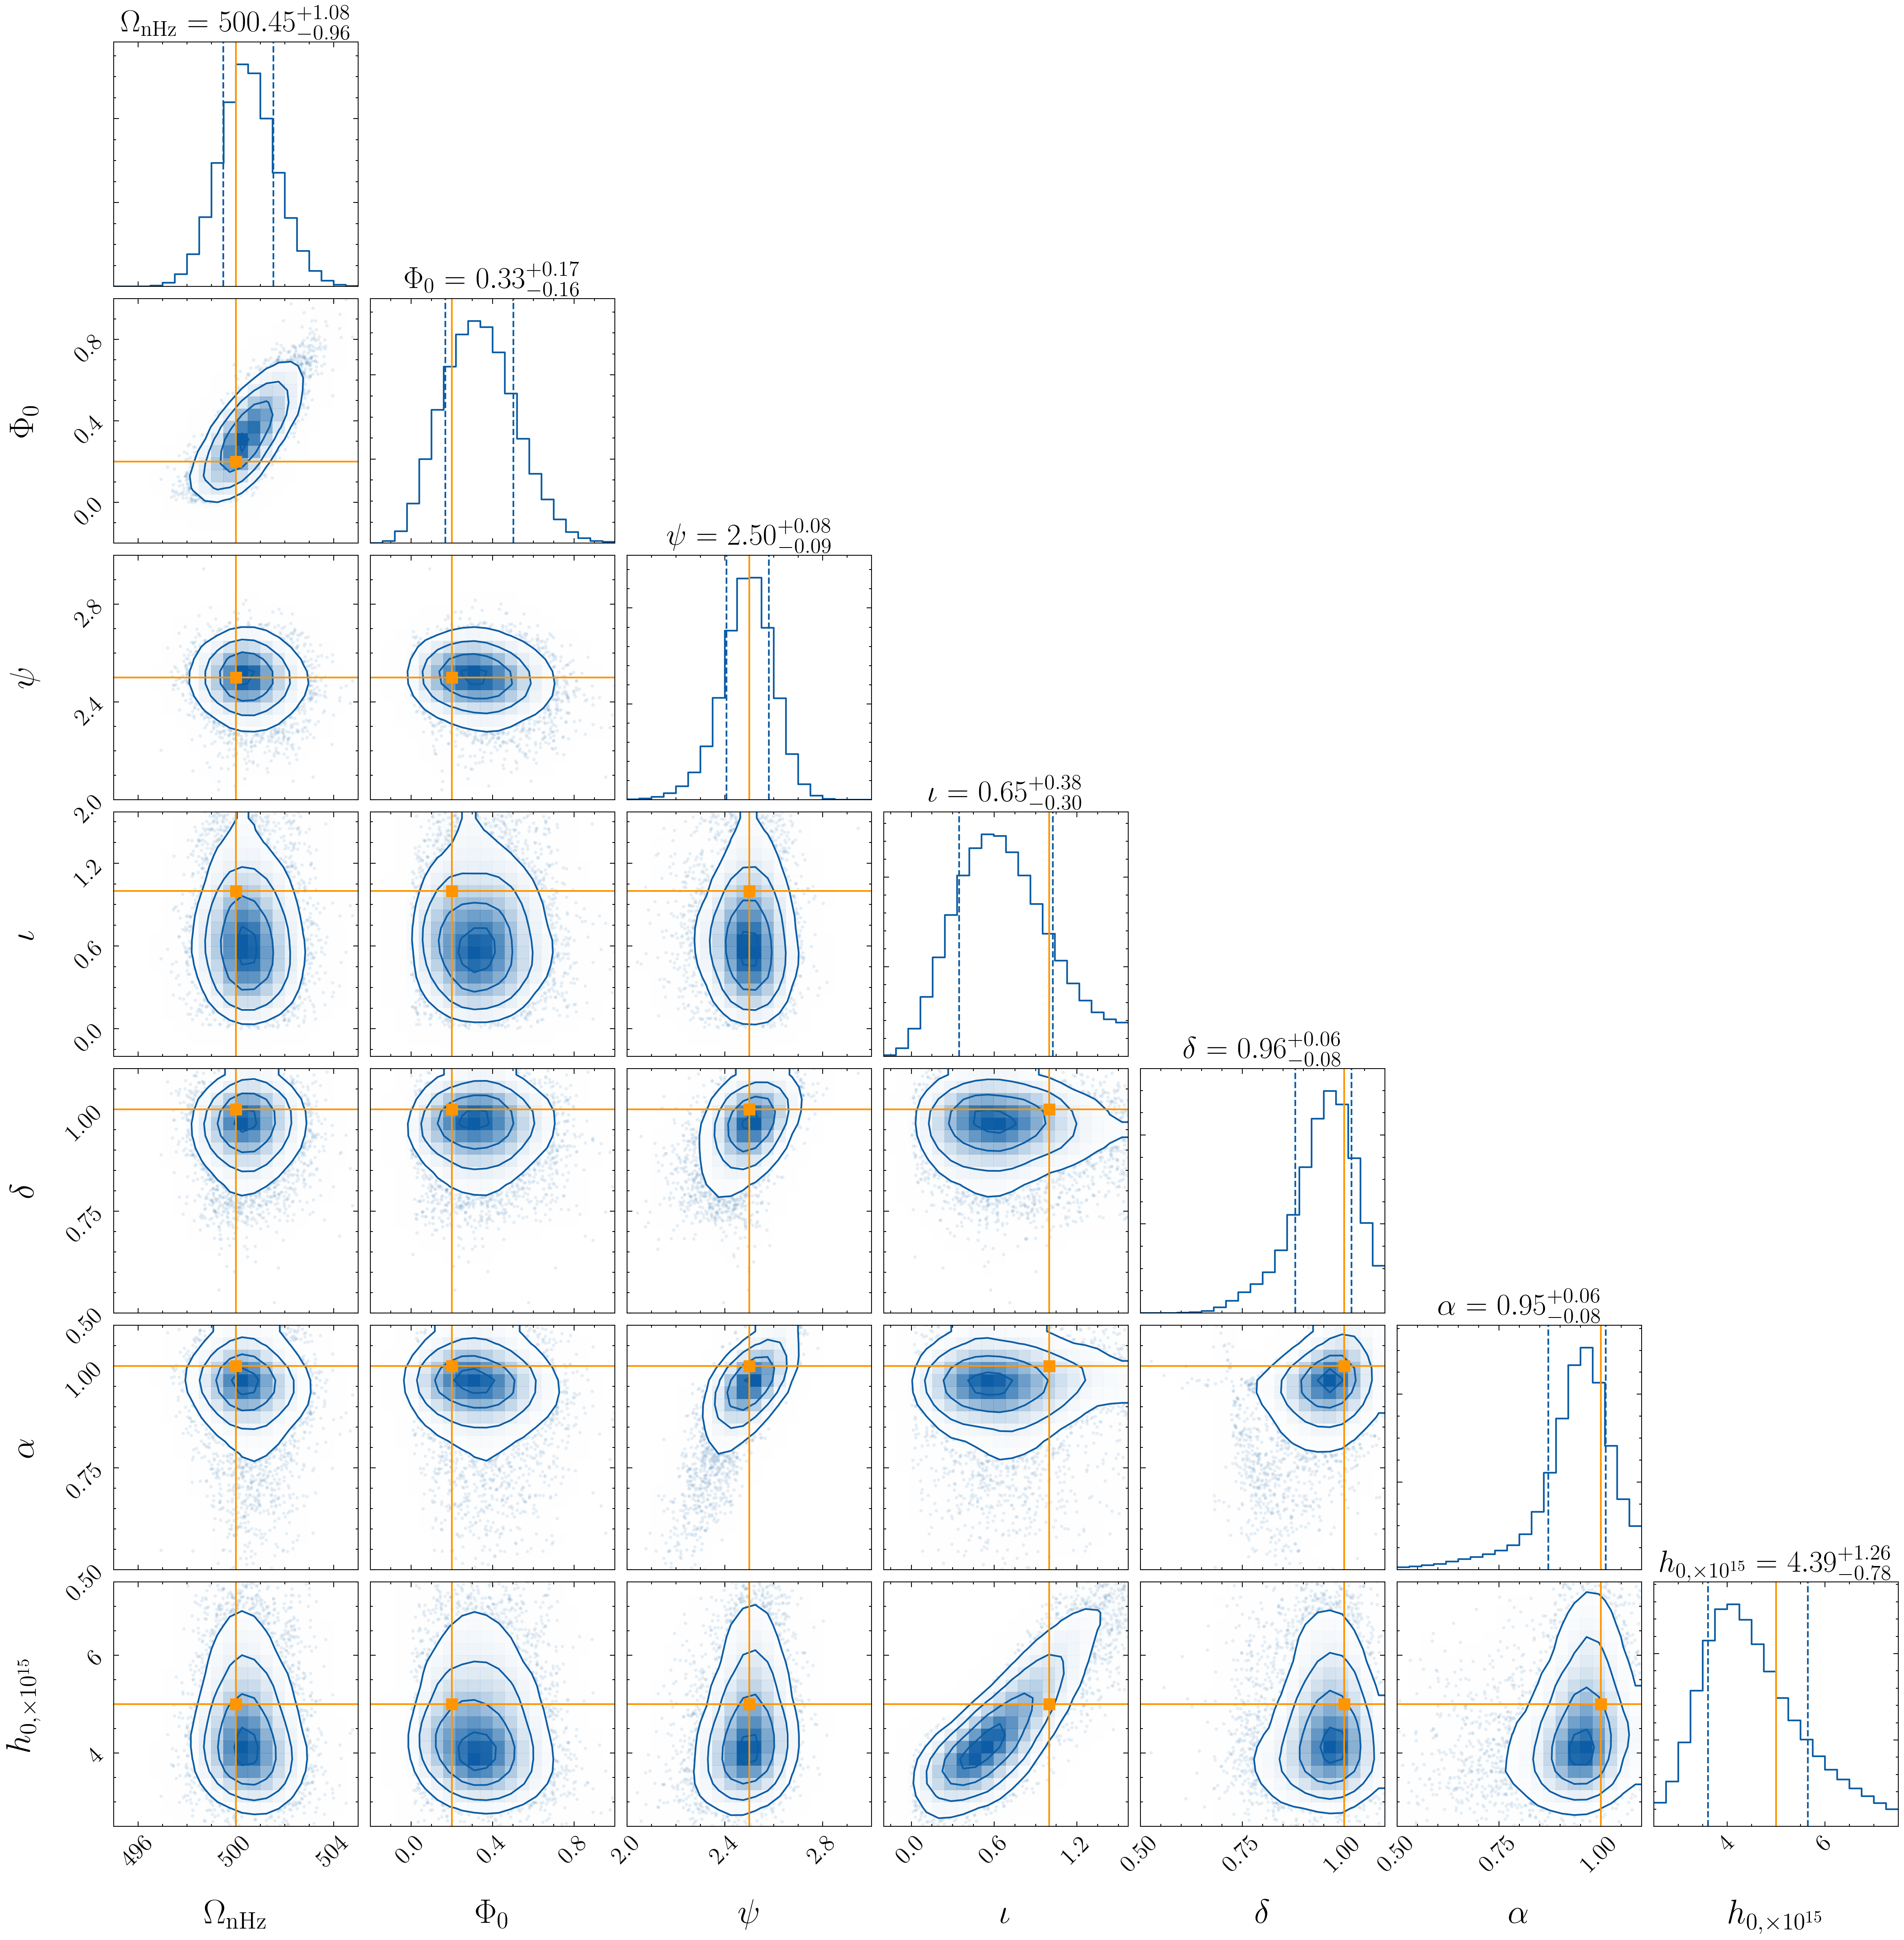
\includegraphics[width=\textwidth, height =\textwidth ]{images/small_h_posterior_10}
	\caption{Posterior distribution of the GW source parameters $\boldsymbol{\theta}_{\rm gw}$ for the representative system in Table \ref{tab:parameters_and_priors}, for a single realisation of the system noise. The horizontal and vertical orange lines indicate the true injected values. The contours in the two-dimensional histograms mark the (0.5, 1, 1.5, 2)-$\sigma$ levels after marginalizing over all but two parameters. The one-dimensional histograms correspond to the joint posterior distribution marginalized over all but one parameter. The supertitles of the marginalized one-dimensional histograms specify the posterior median and the 0.16 and 0.84 quantiles. We plot the scaled variables $\Omega_{\rm nHz} = \Omega \times 10^{9}$ Hz and $h_{0, \times 10^{15}} = h_0 \times 10^{15}$. The Kalman filter and nested sampler estimate accurately all seven parameters in ${\boldsymbol{\theta}}_{\rm gw}$. The horizontal axes span a subset of the prior domain for all seven parameters.}
	\label{fig:corner_plot_1}
\end{figure*}

%\begin{figure*}
%	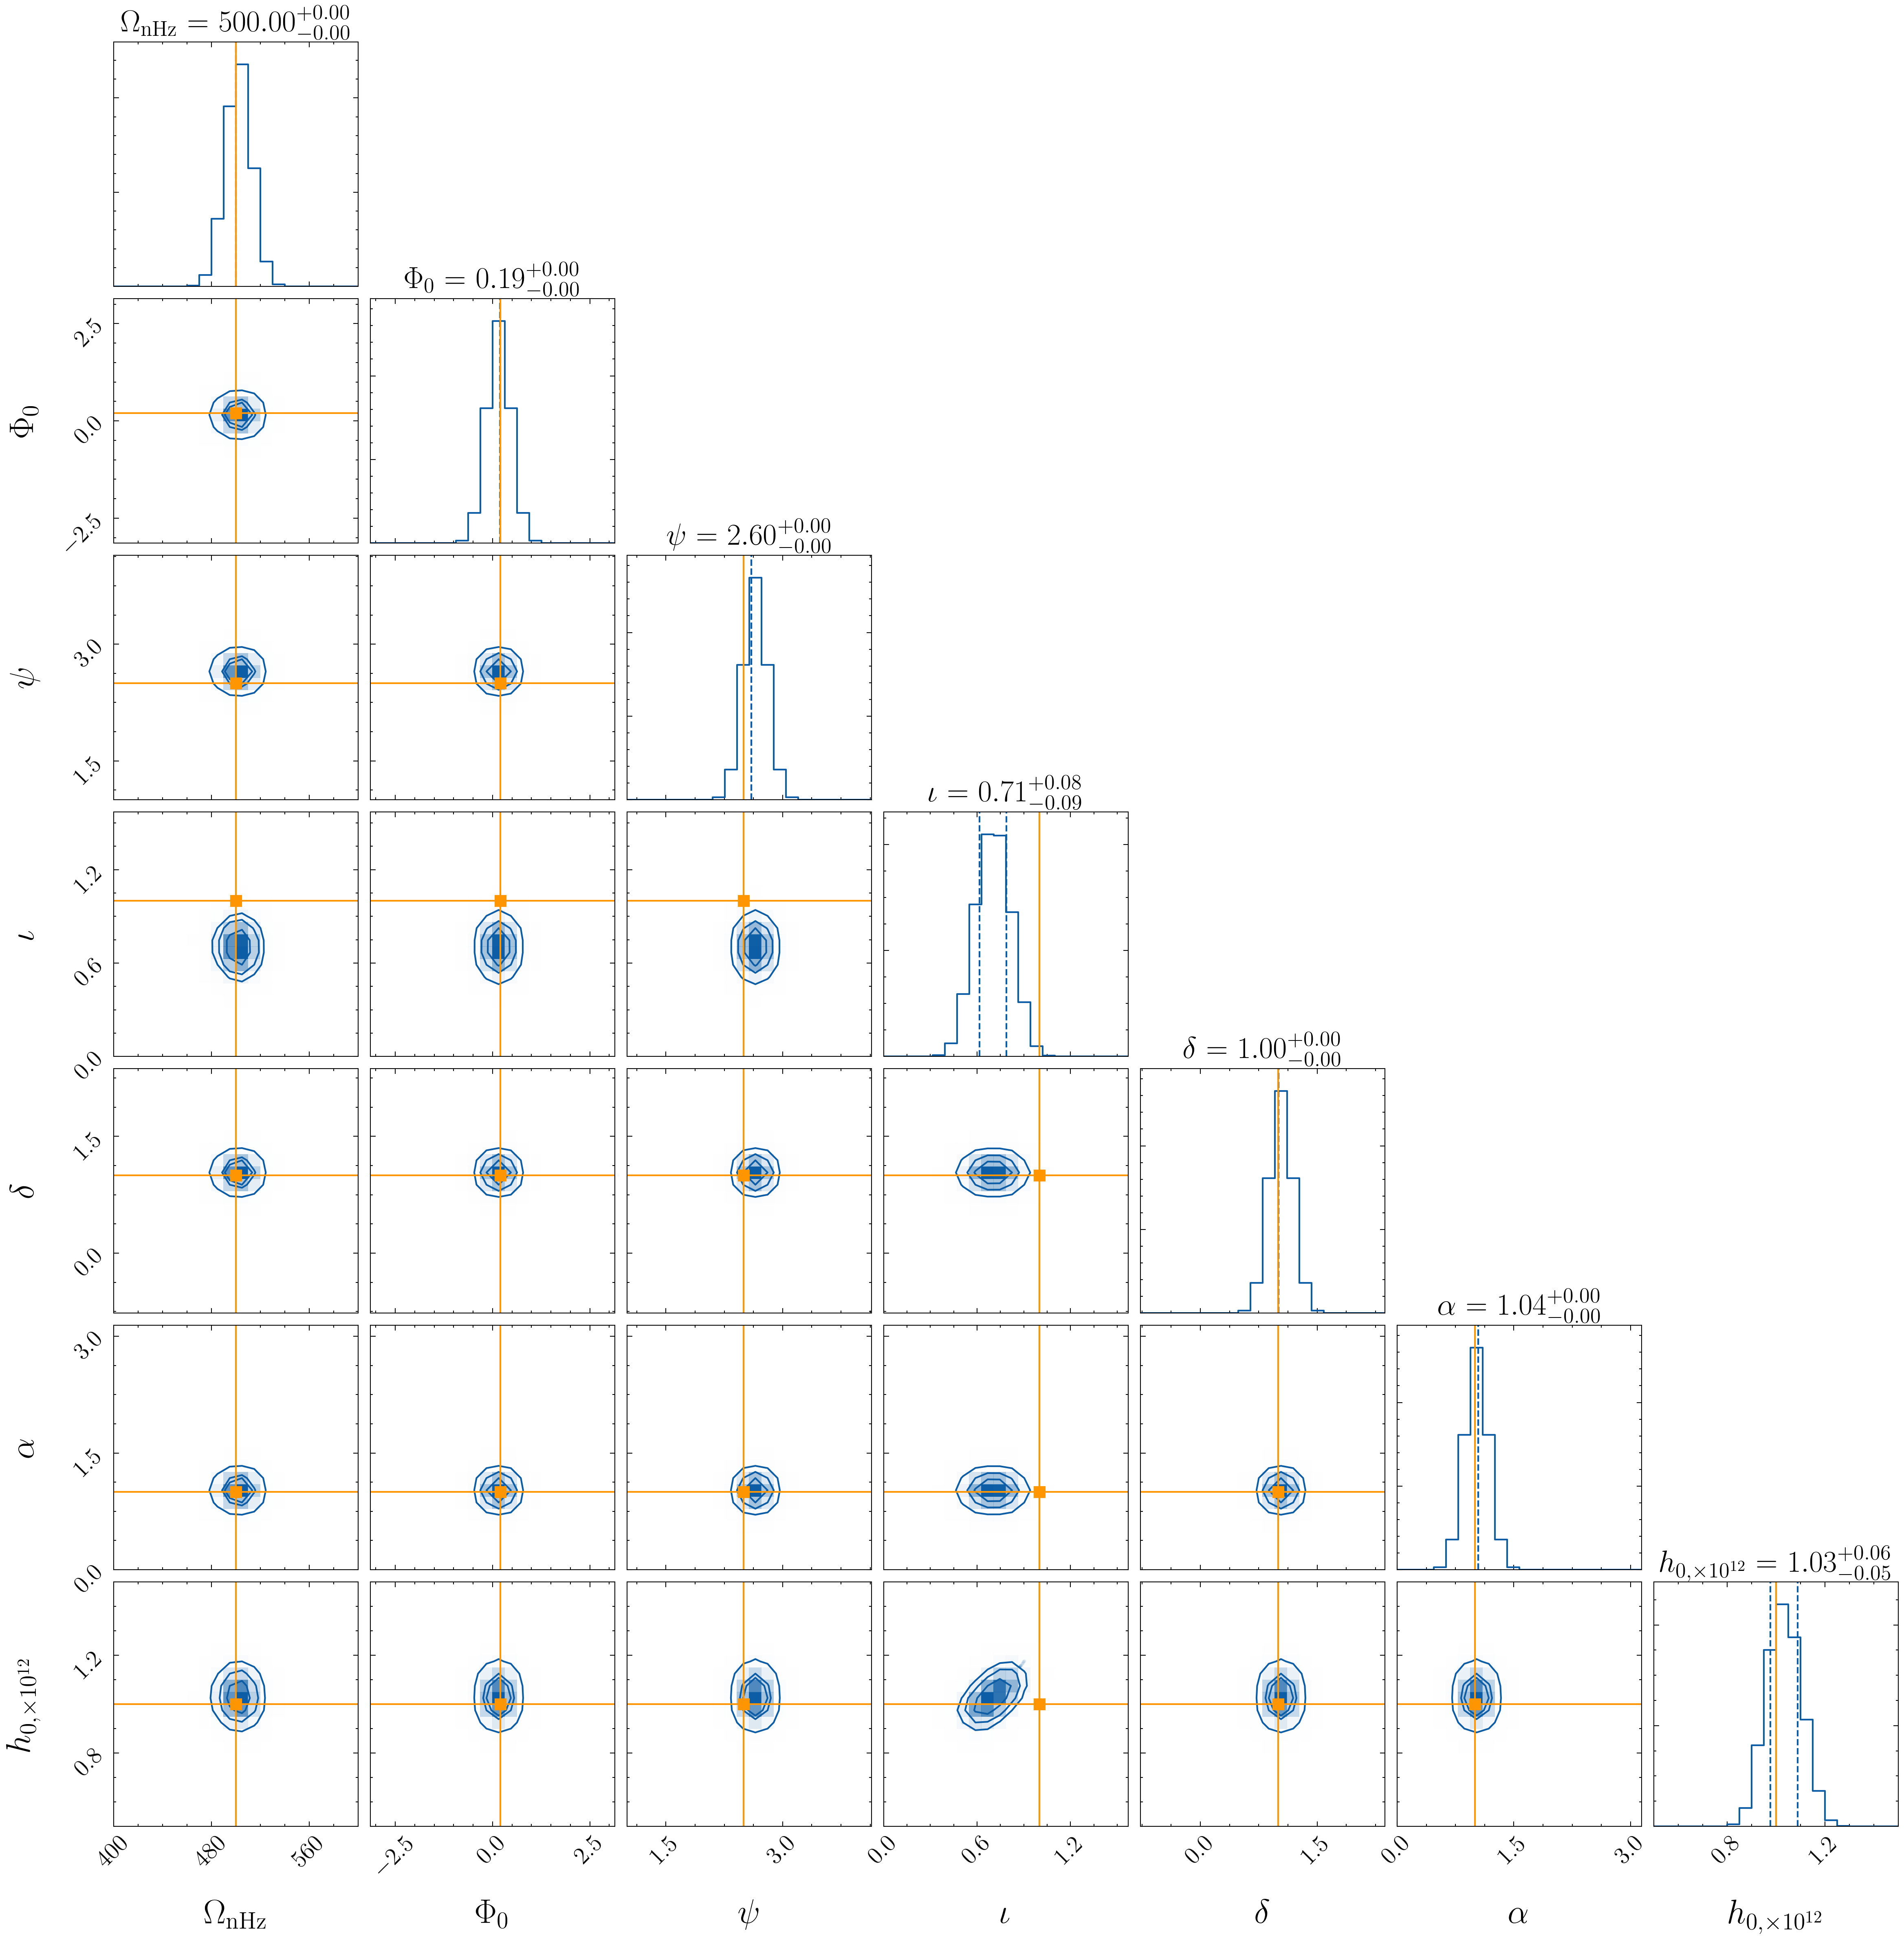
\includegraphics[width=\textwidth, height =\textwidth ]{images/representative_example_v2_GW}
%	\caption{Posterior distribution for the GW source parameters $\boldsymbol{\theta}_{\rm gw}$ for the representative system described in Table \ref{tab:parameters_and_priors}, for a single realisation of the system noise. The vertical orange lines indicate the true injected values. The contours in the 2D histograms denote the (0.5, 1, 1.5, 2)-$\sigma$ levels. We are able to accurately estimate each parameter of interest. We pot the scaled variables $\Omega_{\rm nHz} = \Omega \times 10^{9}$ Hz and $h_{0, \times 10^{12}} = h_0 \times 10^{12}$.}
%	\label{fig:corner_plot_1}
%\end{figure*}



\subsection{Multiple noise realisations: dispersion of outcomes} \label{sec:multiple_noise}
\begin{figure*}
	\includegraphics[width=\textwidth, height =\textwidth]{images/stacked_GW_plot_small_h_definitive3}
	\caption{As Figure \ref{fig:corner_plot_1} but for nine realisations of the noise processes, with curves coloured uniquely. The supertitles of the one-dimensional histograms record the posterior median and the 0.16 and 0.84 quantiles of the median realisation. The known, injected value lies within the 90\% credible interval for 58 out of the 63 combinations of seven parameters and nine noise realizations. There is an appreciable dispersion among the peaks of the one-dimensional posteriors is appreciable, with coefficient of variation $\sim10 \%$ across the 63 combinations. A slight skew-bias is apparent in some of the parameters, e.g. $\iota$. Weak correlations can be seen between $\Omega - \Phi_0$, $\psi-\alpha$ and $\iota - h_0$.} 
	\label{fig:corner_plot_2}
\end{figure*}
\begin{table}
	\centering
	\begin{tabular}{ccll}
		\toprule
		Parameter & Injected Values & Units & $W_{1, \rm median}$  \\
		\hline
		$\Omega$     &   $5 \times 10^{-7}$ & Hz & $10^{-9}$ \\
		$\Phi_0$          & $0.20$ & rad & $0.13$ \\
		$\psi$              & $2.50$ & rad & $0.16$ \\
		$\iota$             & $1.0$ & rad & $0.14$ \\ 
		$\delta$              & $1.0$  & rad & $0.09$ \\
		$\alpha$          & $1.0$  & rad & $0.17$\\
		$h_0$            & $5 \times 10^{-15}$ & - & $8 \times 10^{-16}$ \\
		\bottomrule
	\end{tabular}
	\caption{Median value of the Wasserstein distance $W_{1, \rm median}$, for each parameter in $\boldsymbol{\theta}_{\rm gw}$, calculated across the $10^3 \choose 2$ pairs of probability posteriors, for the $10^3$ noise realisations in Figure \ref{fig:pairwise_wasserstein}. $W_{1, \rm median}$ is generally smaller than the prior domain.}
	\label{tab:Wasserstein}
\end{table}

The results in Section \ref{sec:parameter_estim} are for a single realisation of the noise processes $\xi^{(n)}(t)$ and $\varepsilon^{(n)}(t)$. It is important to confirm that the analysis scheme returns accurate answers for arbitrary noise realisations and that the specific realisation of the noisy data used in Section \ref{sec:parameter_estim} is not particularly advantageous by accident. It is also important to quantify, albeit approximately, the natural random dispersion in the one-dimensional posterior medians from one noise realization to the next, as the dispersion is a practical measure of the accuracy of the parameter estimation scheme, when it is applied to real astronomical data, where the true parameter values and specific noise realisation are unknown. \newline 

To this end we start with the representative example in Table \ref{tab:parameters_and_priors} and generate $1000$ realisations of the process noise $\xi^{(n)}(t)$ and measurement noise $\varepsilon^{(n)}(t)$. For each realisation we independently estimate the static parameters, $\boldsymbol{\theta}$. In Figure \ref{fig:corner_plot_2} we plot the estimates of $\boldsymbol{\theta}_{\rm gw}$ for nine arbitrary realisations. The corner plot is arranged identically to Figure \ref{fig:corner_plot_1}, which stems from one realisation. We plot nine realisations rather than the full set of 1000 to avoid overcrowding. As in Section \ref{sec:parameter_estim}, $\boldsymbol{\theta}_{\rm gw}$ is also recovered unambiguously across the 1000 noise realisations, but for the sake of brevity we do not show the results here. \newline 


Figure \ref{fig:corner_plot_2} confirms two main points (i) the results from the nine noise realisations overlap with the single realisation in  Figure \ref{fig:corner_plot_1}; and (ii) the dispersion among the peaks of the one-dimensional posteriors is appreciable, with variations of $\sim10 \%$ (coefficient of variation) across the seven parameters and nine realizations. Indeed, considering the one-dimensional marginalized posteriors, we find that the injected value is contained within the 90\% credible interval in 58 out of the 63 (i.e. $92 \%$) possible combinations of the seven parameters and nine realizations. Figure \ref{fig:corner_plot_2}, like Figure \ref{fig:corner_plot_1}, displays tentative signs of bias, where the one-dimensional posteriors are not symmetric about the injected value. For example, the maximum a posteriori probability estimates of $\iota$ appear left-skewed, consistently underestimating the injected value in all nine realisations. A similar but messier trend is seen in $\delta$. However, the width of the posteriors is comparable to the putative bias, so it is difficult to draw strong conclusions. Bias is discussed in detail in Section \ref{sec:bias}. There is no strong evidence for correlations between parameter pairs, e.g.\ banana-shaped contours. \newline 


We now consider the complete set of $10^3$ noise realisations, going beyond than the subset of nine realisations in the preceding discussion. We ask the question: how ``similar'' are the $10^3$ marginalized, one-dimensional posteriors computed for each of the seven parameters in ${\boldsymbol{\theta}}_{\rm gw}$? There is no unique way to answer this question. In this paper we appeal to the Wasserstein distance \citep[WD;][]{Wasserstein,Villani2009} from optimal transport theory, which defines an intuitive notion of similarity between probability distributions. The WD is a popular metric in machine learning \citep{2017arXiv170107875A}, climate modelling \citep{2022JCli...35.1215P,2023QJRMS.149..843K}, computational biology \citep{GONZALEZDELGADO2023168053} and geophysics \citep{2023GeoRL..5003880M}; a short review is presented in Appendix \ref{sec:wasserstein}. The WD measures the cost of an optimal strategy for moving probability mass between two distributions from position $x$ to position $y$, with respect to some cost function $c(x,y)$. In this paper we use the first WD moment, $W_1(\mu,\nu)$, which is defined and interpreted in Appendix \ref{sec:wasserstein}. Intuitively $W_1$ bounds the difference in the expectation value of a parameter selected from ${\boldsymbol{\theta}}_{\rm gw}$" with respect to the PDFs $\mu$ and $\nu$. Taking a concrete example, suppose that we infer two one-dimensional posterior distributions $\mu(\iota)$ and $\nu(\iota)$ for $\iota$, for two different realisations of the noise, and calculate $W_1(\mu, \nu) =0.5$ rad. Then we can infer $| \langle \iota \rangle_\mu - \langle \iota \rangle_\nu | \leq 0.5 \, {\rm rad}$. \newline 


Table \ref{tab:Wasserstein} summarizes the WD between the $5\times 10^5$ pairs of one-dimensional posteriors across the $10^3$ realizations, for each of the seven parameters in ${\boldsymbol{\theta}}_{\rm gw}$. The median $W_1$ for each parameter is tabulated in the rightmost column and denoted by $W_{1,{\rm median}}$. As a percentage of the known, injected value, $W_{\rm 1,median}$ ranges from  0.2\% for $\Omega$ to 67\% for $\Phi_0$. These values are an approximate measure of the natural dispersion in parameter estimates when the analysis scheme is applied to real, astronomical data, where the true parameter values are unknown. Moreover, as a percentage of the prior domain, $W_{\rm 1,median}$ ranges from $8.14 \times 10^{-4}$ \% for $h_0$ to 2.69\% for $\psi$. These values serve as confirmation that the nested sampler converges reliably to a single, narrow peak without railing against the prior bounds for a wide variety of noise realizations. Further analysis of the WD is performed in Appendix \ref{sec:wasserstein}.



\subsection{Detectability versus $h_0$} \label{sec:detection}
We frame the problem of detecting a GW in noisy PTA data in terms of the Bayesian model selection procedure described in Section \ref{sec:model_selection}. In Equatin \eqref{eq:bayes} $\mathcal{M}_1$ is the Earth-terms-only model, i.e. the state-space model with a Kalman filter based on Equation \eqref{eq:measuremen_earth}. The Bayes factor, $\beta$, as defined in Equation \eqref{eq:bayes} is presented in Figure \ref{fig:bayes} for the representative source in Table \ref{tab:parameters_and_priors}, except that we now vary the source amplitude, $h_0$, from $10^{-15}$ (undetectable) to $10^{-12}$ (easily detectable). To control the test, the noise processes in the synthetic data are identical realisations for each value of $h_0$; the only change from one $h_0$ value to the next is $h_0$ itself. \footnote{Changing the noise realizations as well, from one value of $h_0$ to the next, simply adds uninformative scatter to the trend in Figure \ref{fig:bayes}.} \newline 

	
We see in Figure \ref{fig:bayes} an approximate quadratic relationship $\beta \propto h_0^2$ exists. The GW source is detectable with decisive evidence ($\beta \geq 10$) for $h_0 \gtrsim 4 \times 10^{-15}$. Of course, the minimal detectable strain is particular to the system in Table \ref{tab:parameters_and_priors}. It is influenced in general by e.g. $T_{\rm obs}$, ${\boldsymbol{\theta}}_{\rm gw}$, and ${\boldsymbol{\theta}}_{\rm psr}$, as discussed in Section \ref{sec:parameter_space}. Adjusting $\sigma_{\rm m}$ linearly scales the effective signal-to-noise ratio $h_0 / \sigma_{\rm m}$, such that an approximate quadratic relationship $\beta \propto h_0^2 / \sigma_{\rm m}^2$ also exists. \newline 


The odds ratio $\beta$ drops off for $h_0 \lesssim 4 \times10^{-15}$. This happens because the two competing models becoming increasingly indistinguishable once the measurement noise dominates the GW signal. Moreover, the points in Figure \ref{fig:bayes} become sparser for $h_0 \lesssim 4 \times 10^{-15}$. This happens because we find $\beta <0$ for the missing, intermediate points. This is a noise artefact of the nested sampler.When the sampler converges sub-optimally, the hierarchical relationship between $\mathcal{M}_0$ and  $\mathcal{M}_1$ fails, and $\mathcal{Z}(\boldsymbol{Y} | \mathcal{M}_1) > \mathcal{Z}(\boldsymbol{Y} | \mathcal{M}_0)$ no longer holds. There is nothing special about the particular missing points; if one recreates the $\beta(h_0)$ curve by rerunning the nested sampler with another random seed, a different set of points are missing. Increasing the number of live points $n_{\rm live}$ used by the nested sampler improves the performance at small values of $h_0$, because the uncertainties in $\mathcal{Z}$ scale as $\mathcal{O}(n_{\rm live}^{-1/2})$ (see Section \ref{sec:nested_sampling}). In this section we set $n_{\rm live} =2000$. 
\begin{figure}
	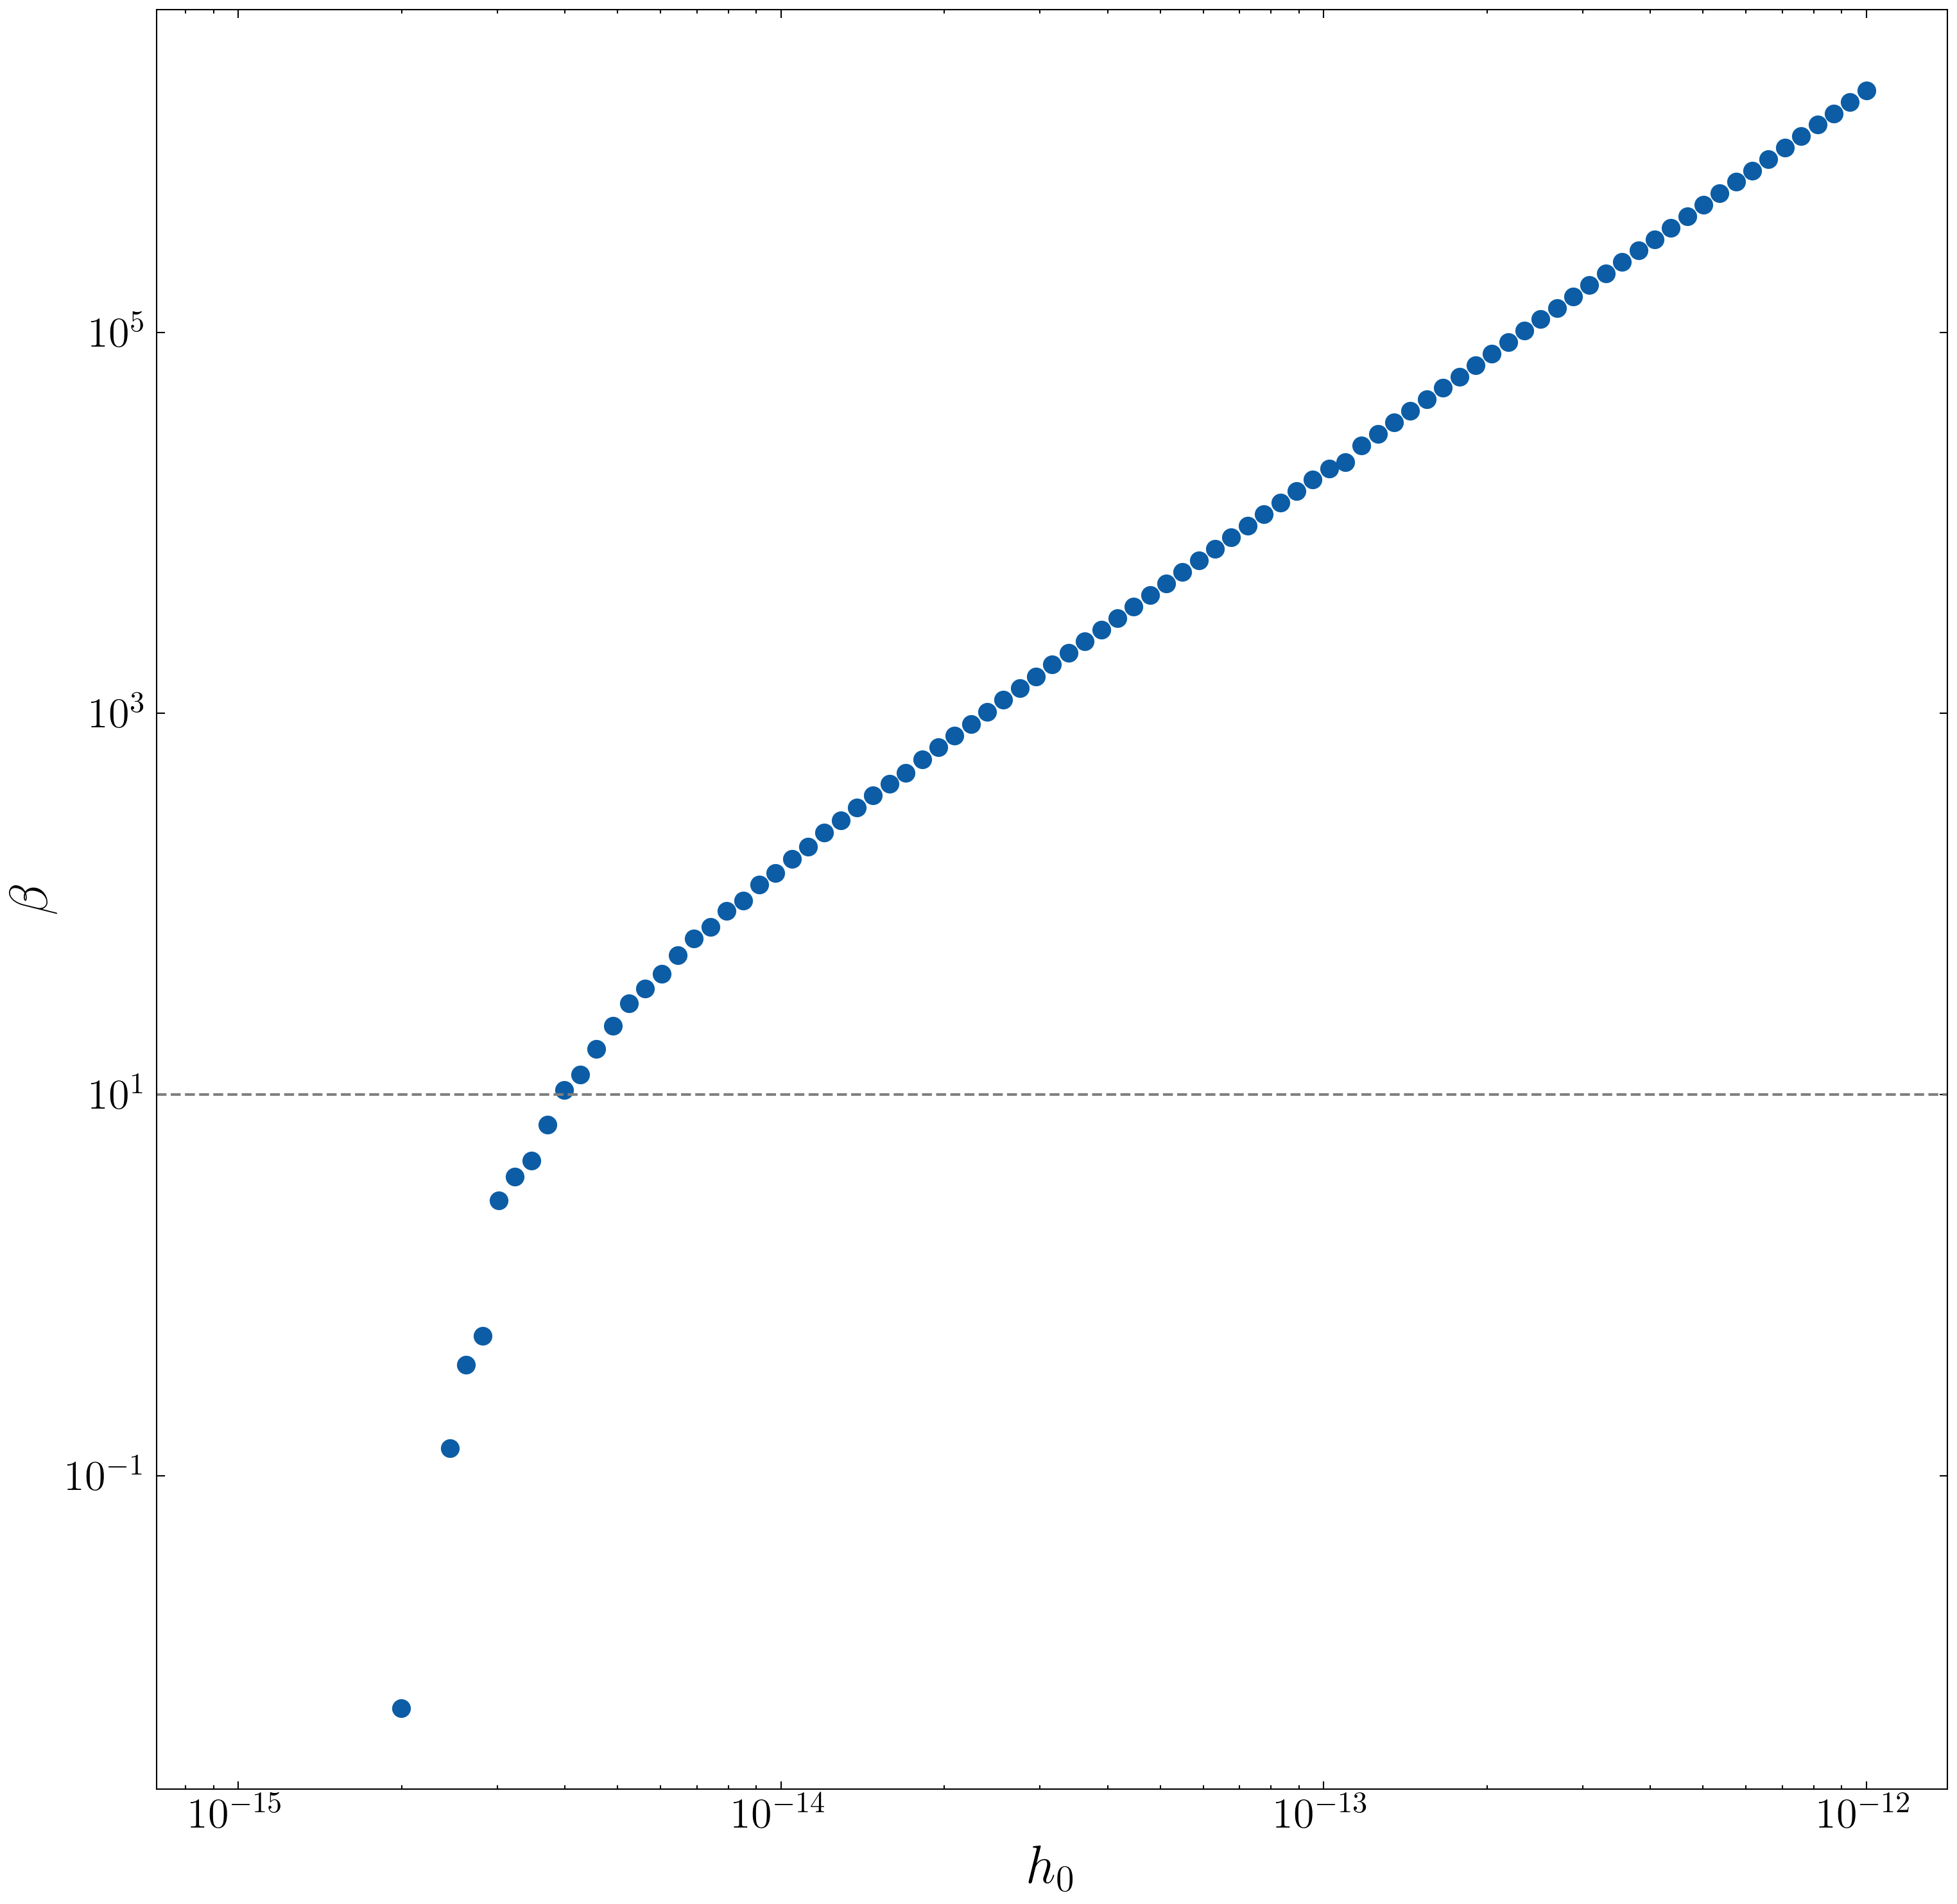
\includegraphics[width=\columnwidth]{images/CanonicalBayesPlot2000}
	\caption{Bayes factor (odds ratio) $\beta$ between the competing models $\mathcal{M}_1$ (GW present in data) and $\mathcal{M}_0$ (GW not present in data) at different GW amplitudes, $h_0$, for the representative example in Table \ref{tab:parameters_and_priors}. The horizontal grey dashed line labels an arbitrary detection threshold, $\beta = 10$. The minimum detectable strain for $\beta < 10$, is $ 4 \times 10^{-15}$. Missing points for $\beta\leq 10$ occur when noise subverts the hierarchical relationship between $\mathcal{M}_0$ and $\mathcal{M}_1$ (see Section \ref{sec:detection}).}
	\label{fig:bayes}
\end{figure}


\section{Exploring a broader parameter space} \label{sec:parameter_space}
\begin{figure}
	\centering
	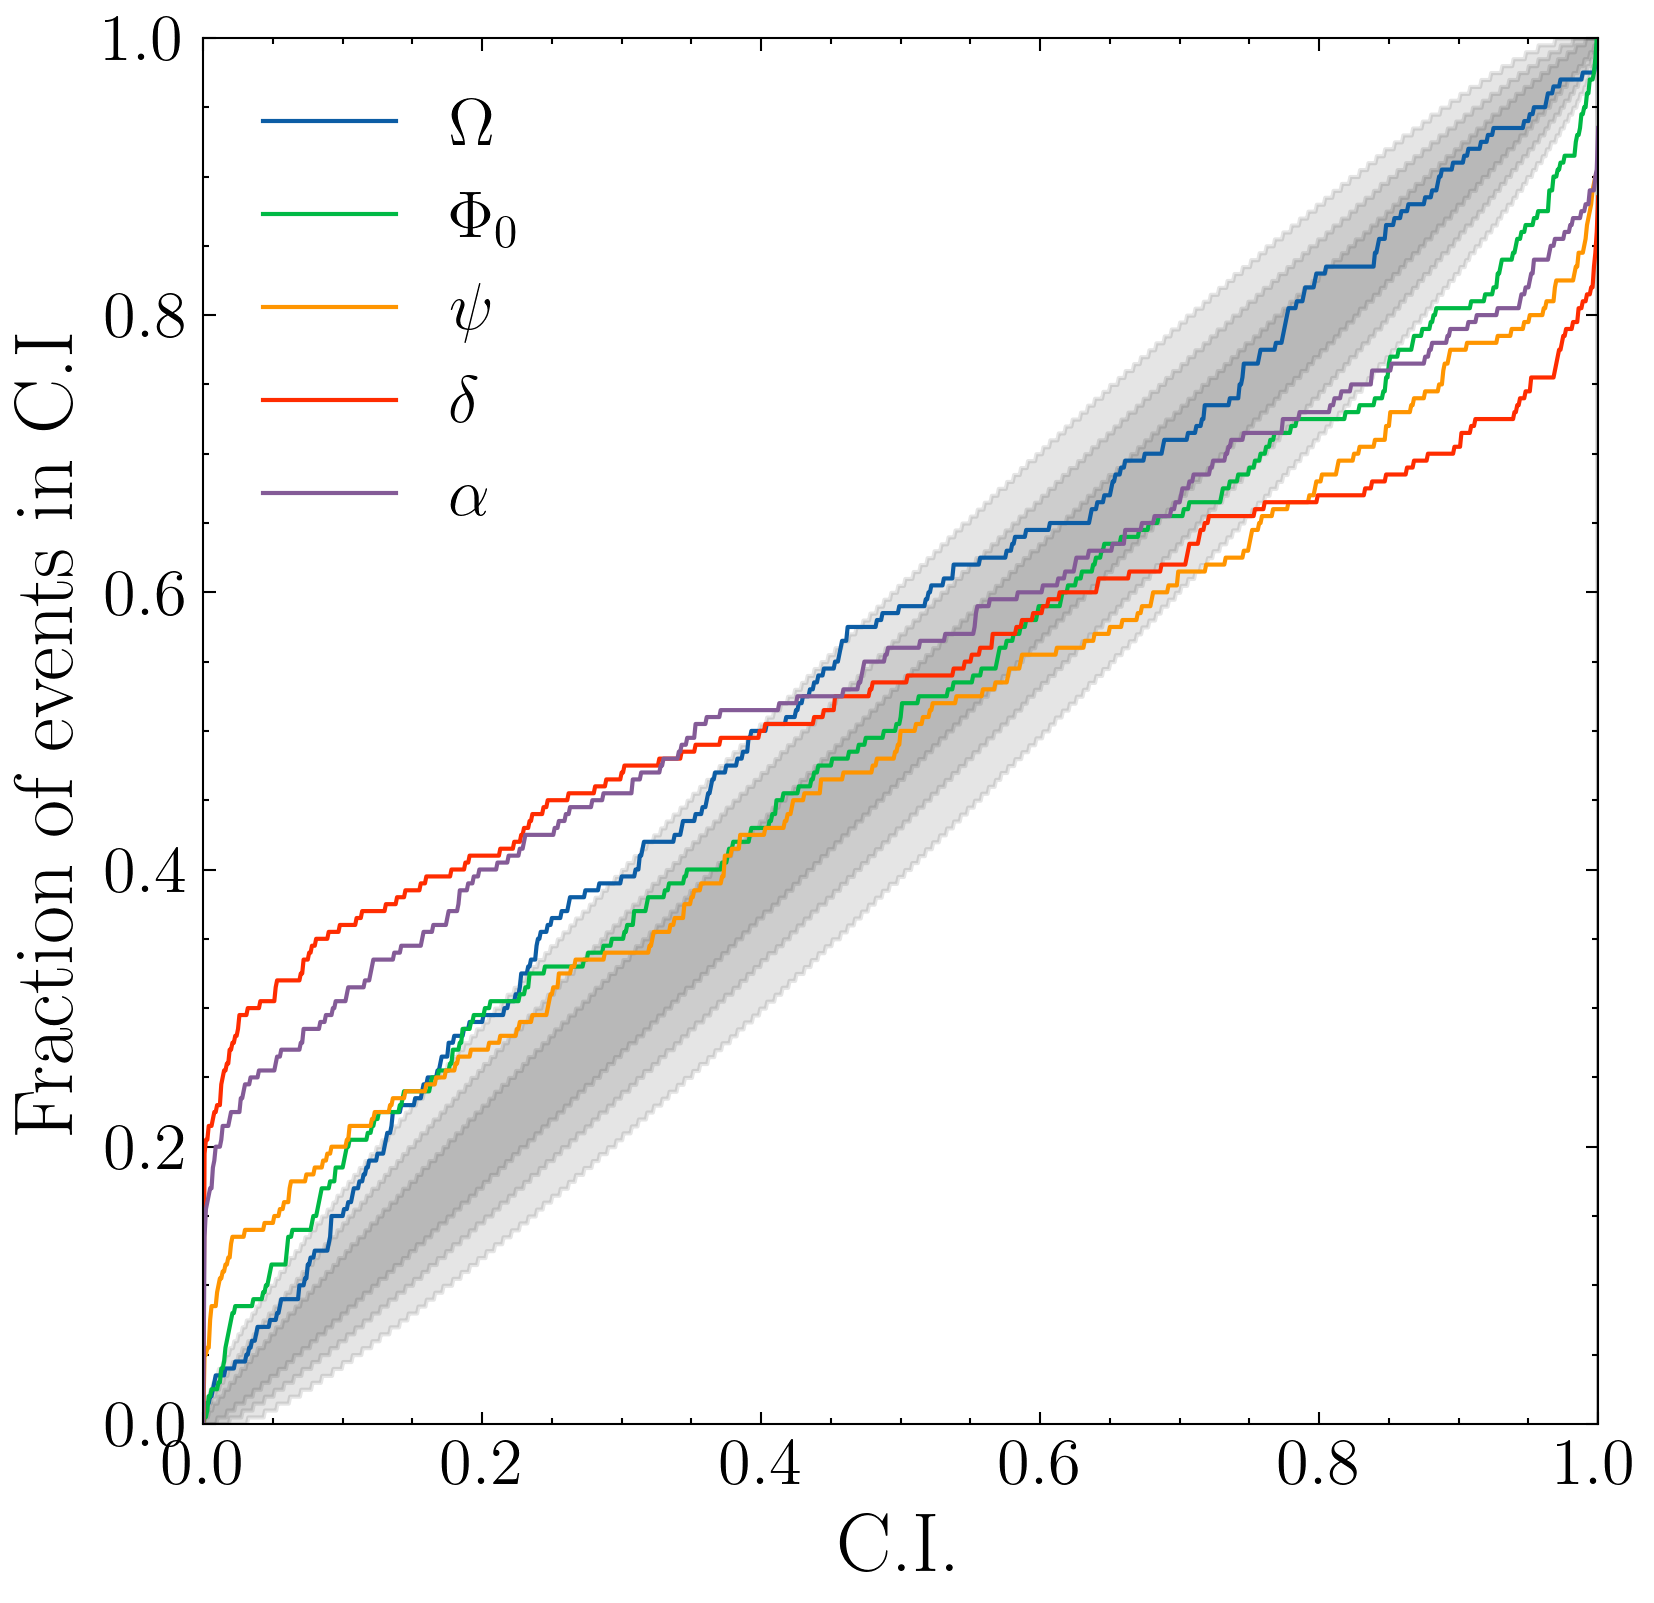
\includegraphics[width=\columnwidth]{images/pp_plot_new}
	\caption{PP plot for 200 simulated GW sources for a subset of parameters of $\boldsymbol{\theta}_{\rm gw}$, randomly drawn from the prior distributions of Table \ref{tab:parameters_and_priors}. Each coloured line corresponds to a different parameter of $\boldsymbol{\theta}_{\rm gw}$. The parameters $h_0$ and $\iota$ are fixed at $5 \times 10^{-15}$ and 1.0 rad respectively in order to maintain an approximately constant SNR. The grey shaded contours labels the $1,2,3$-$\sigma$ confidence intervals. Well estimated posteriors should fall along the diagonal $y=x$. $\Omega$ is generally well-estimated but many other parameters show evidence of being over-constrained due to a modelling bias. }
	\label{fig:parameter_space}
\end{figure}
We have so far focussed on a single representative system, summarised in Table \ref{tab:parameters_and_priors}. In this section we test the method in different regions of the parameter space, varying the source parameters through astrophysically relevant ranges. \newline 


We consider 200 injections for different sets of parameter values where we fix $h_0 = 5 \times 10^{-15}$, $\iota =1.0$ and draw the remaining five parameters of $\boldsymbol{\theta}_{\rm gw}$ from the prior distributions described in Table \ref{tab:parameters_and_priors}. We fix $h_0$ and $\iota$ in order to maintain an approximately constant SNR across the parameter space. For each simulated injection we can then attempt to recover the posterior distributions for each parameter. To summarise the results across the parameter space we use a parameter-parameter (PP) plot \citep{doi:10.1198/106186006X136976}. A PP plot describes the fraction of the total number of injected parameters which are included within a given credible interval of the estimated posterior with respect to the credible interval itself. In the ideal case the PP plot should be a diagonal line, indicating that $x$-percentage of the simulated injections fall within the $x$-percentage credible interval. The results are shown in Figure \ref{fig:parameter_space}. The shaded grey contours enclose the $1\sigma$, $2\sigma$, and $3\sigma$ significance levels, given 200 injections. We can see that only $\Omega$ falls within the $3\sigma$ shaded region. The other parameters deviate from the $y=x$ diagonal. The effect is most pronounced for $\alpha$ and $\delta$ with more modest deviations for $\psi$ and $\Phi_0$. The shape of the graph indicates that the posteriors for these parameters are over-constrained; there are fewer injections contained within high value credible intervals than would be expected statistically, and there are more injections contained within the low value credible intervals. This is an result of the bias that we observed in Section \ref{sec:multiple_noise}; the posteriors inferred for these parameters are generally confident, but are systematically biased away from the true injection values. This manifests in the PP plot as posteriors which are overly precise (narrow) to contain the injected value within the appropriate credible interval. An in-depth discussion on the origin of this bias is given in Section \ref{sec:bias}. 


\section{Identifiability and bias} \label{sec:bias_and_identifiability}
There are two underlying issues in the preceding tests that we now explore in more detail. The first relates to parameter identifiability, i.e. can we uniquely identify the parameters of the model given the data and the model structure? This question is explored in Section \ref{sec:identif}. The second relates to a bias in the parameter estimates that results from dropping the pulsar terms from the Kalman filter measurement equation as described in Section \ref{sec:parameter_estim}. This is the focus of Section \ref{sec:bias}. In order to elucidate these questions without confusion from the measurement noise, we now work in the high SNR regime and set $h_0 = 10^{-12}$ (c.f. Figure \ref{fig:bayes}) for our representative example system (Table \ref{tab:parameters_and_priors}).

\subsection{Identifiability}\label{sec:identif}
\begin{figure}
	\centering
	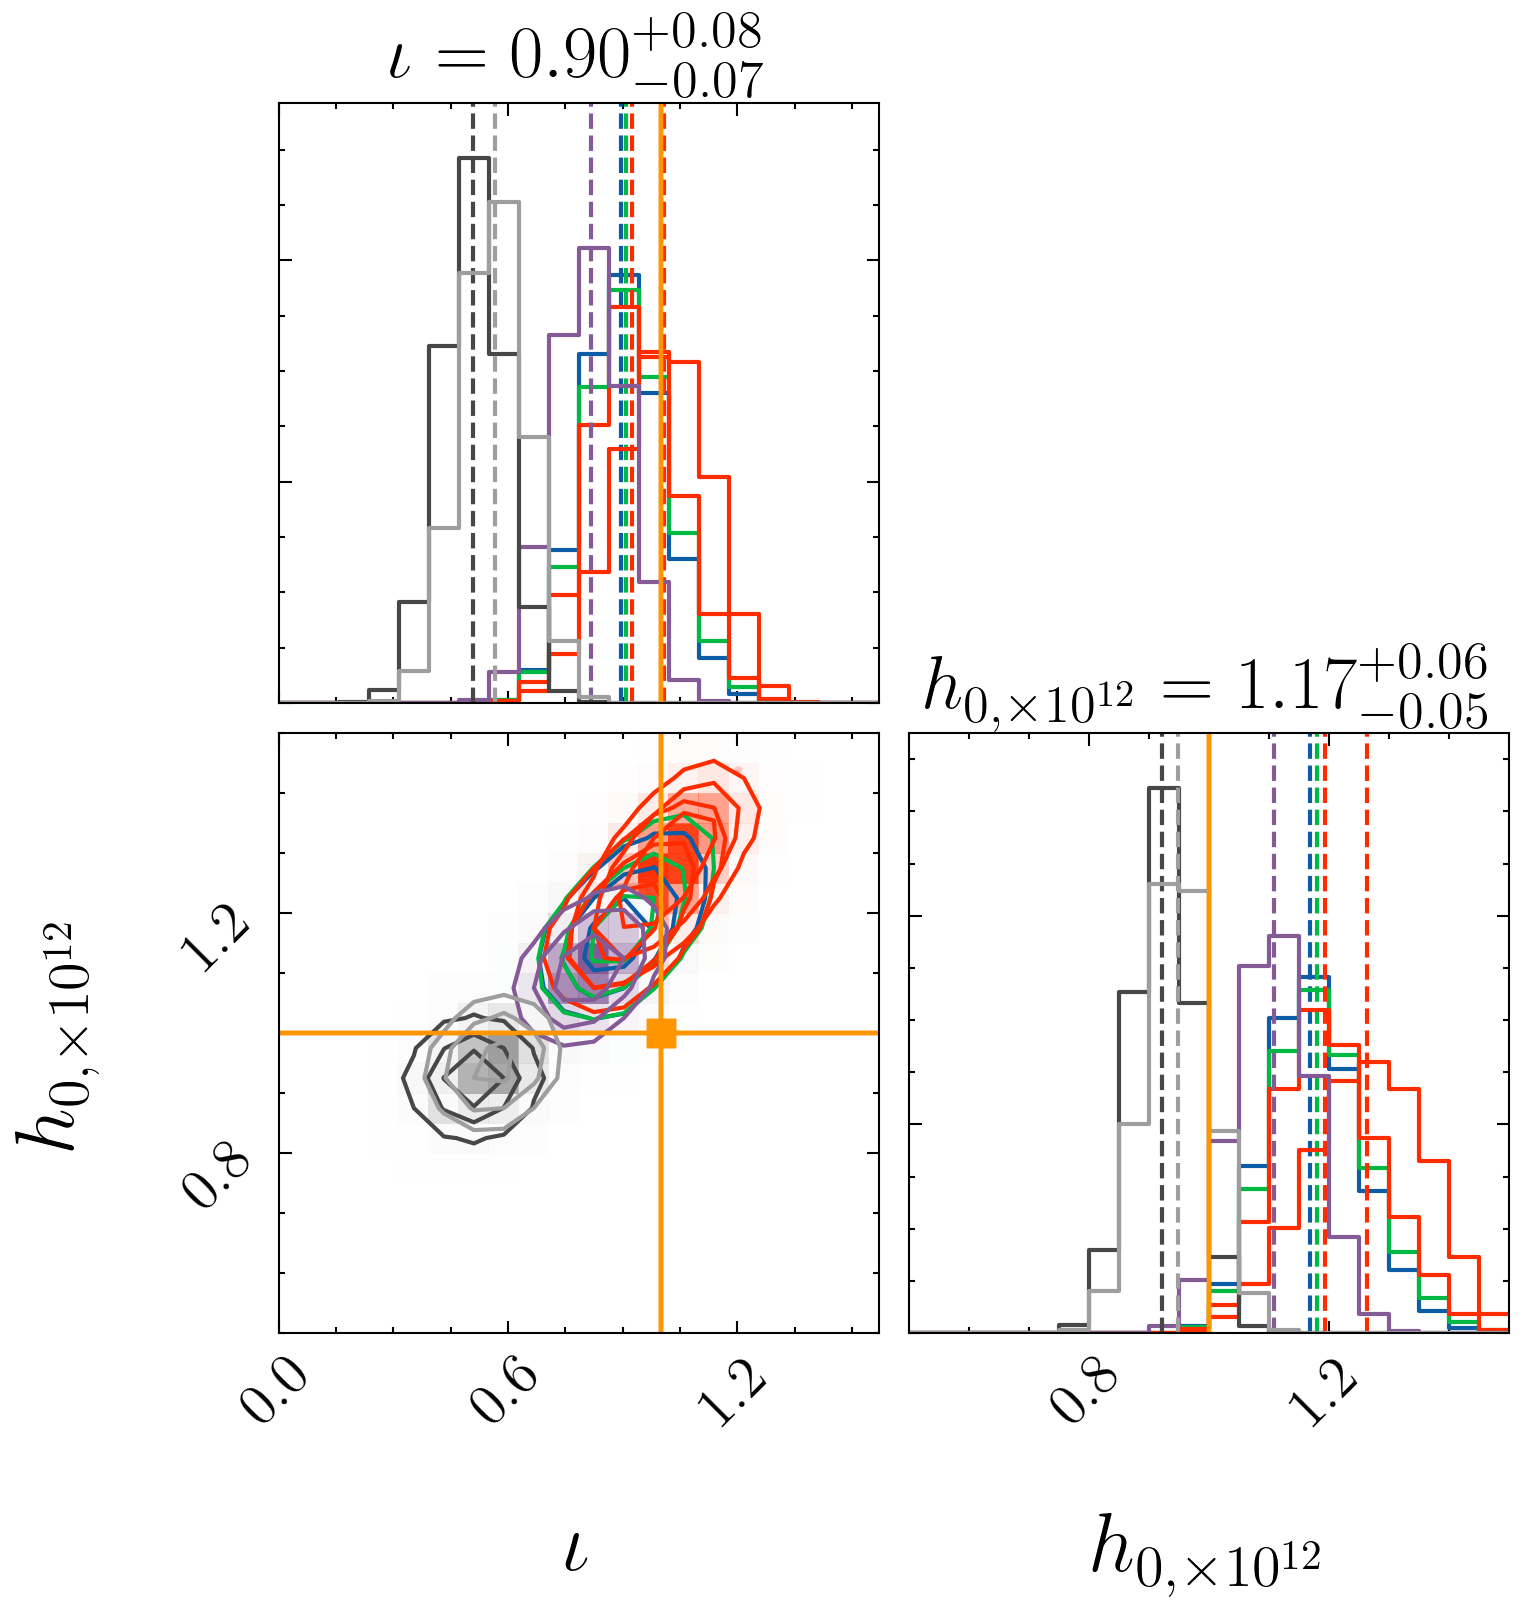
\includegraphics[width=\columnwidth]{images/stacked_GW_plot_iota_h}
	\caption{Posterior probability distributions for the representative system described in Table \ref{tab:parameters_and_priors} over nine noise realisations for the GW source parameters $\iota$ and $h_0$ in the high SNR regime ($h_0 = 10^{-12}$). Unlike the other parameters of  $\boldsymbol{\theta}_{\rm gw}$, the one-dimensional posteriors for $\iota$ and $h_0$ do not strongly overlap. A correlation between  $\iota$ and $h_0$ is evident.}
	\label{fig:just_iota_h}
\end{figure}
\begin{figure}
	\centering
	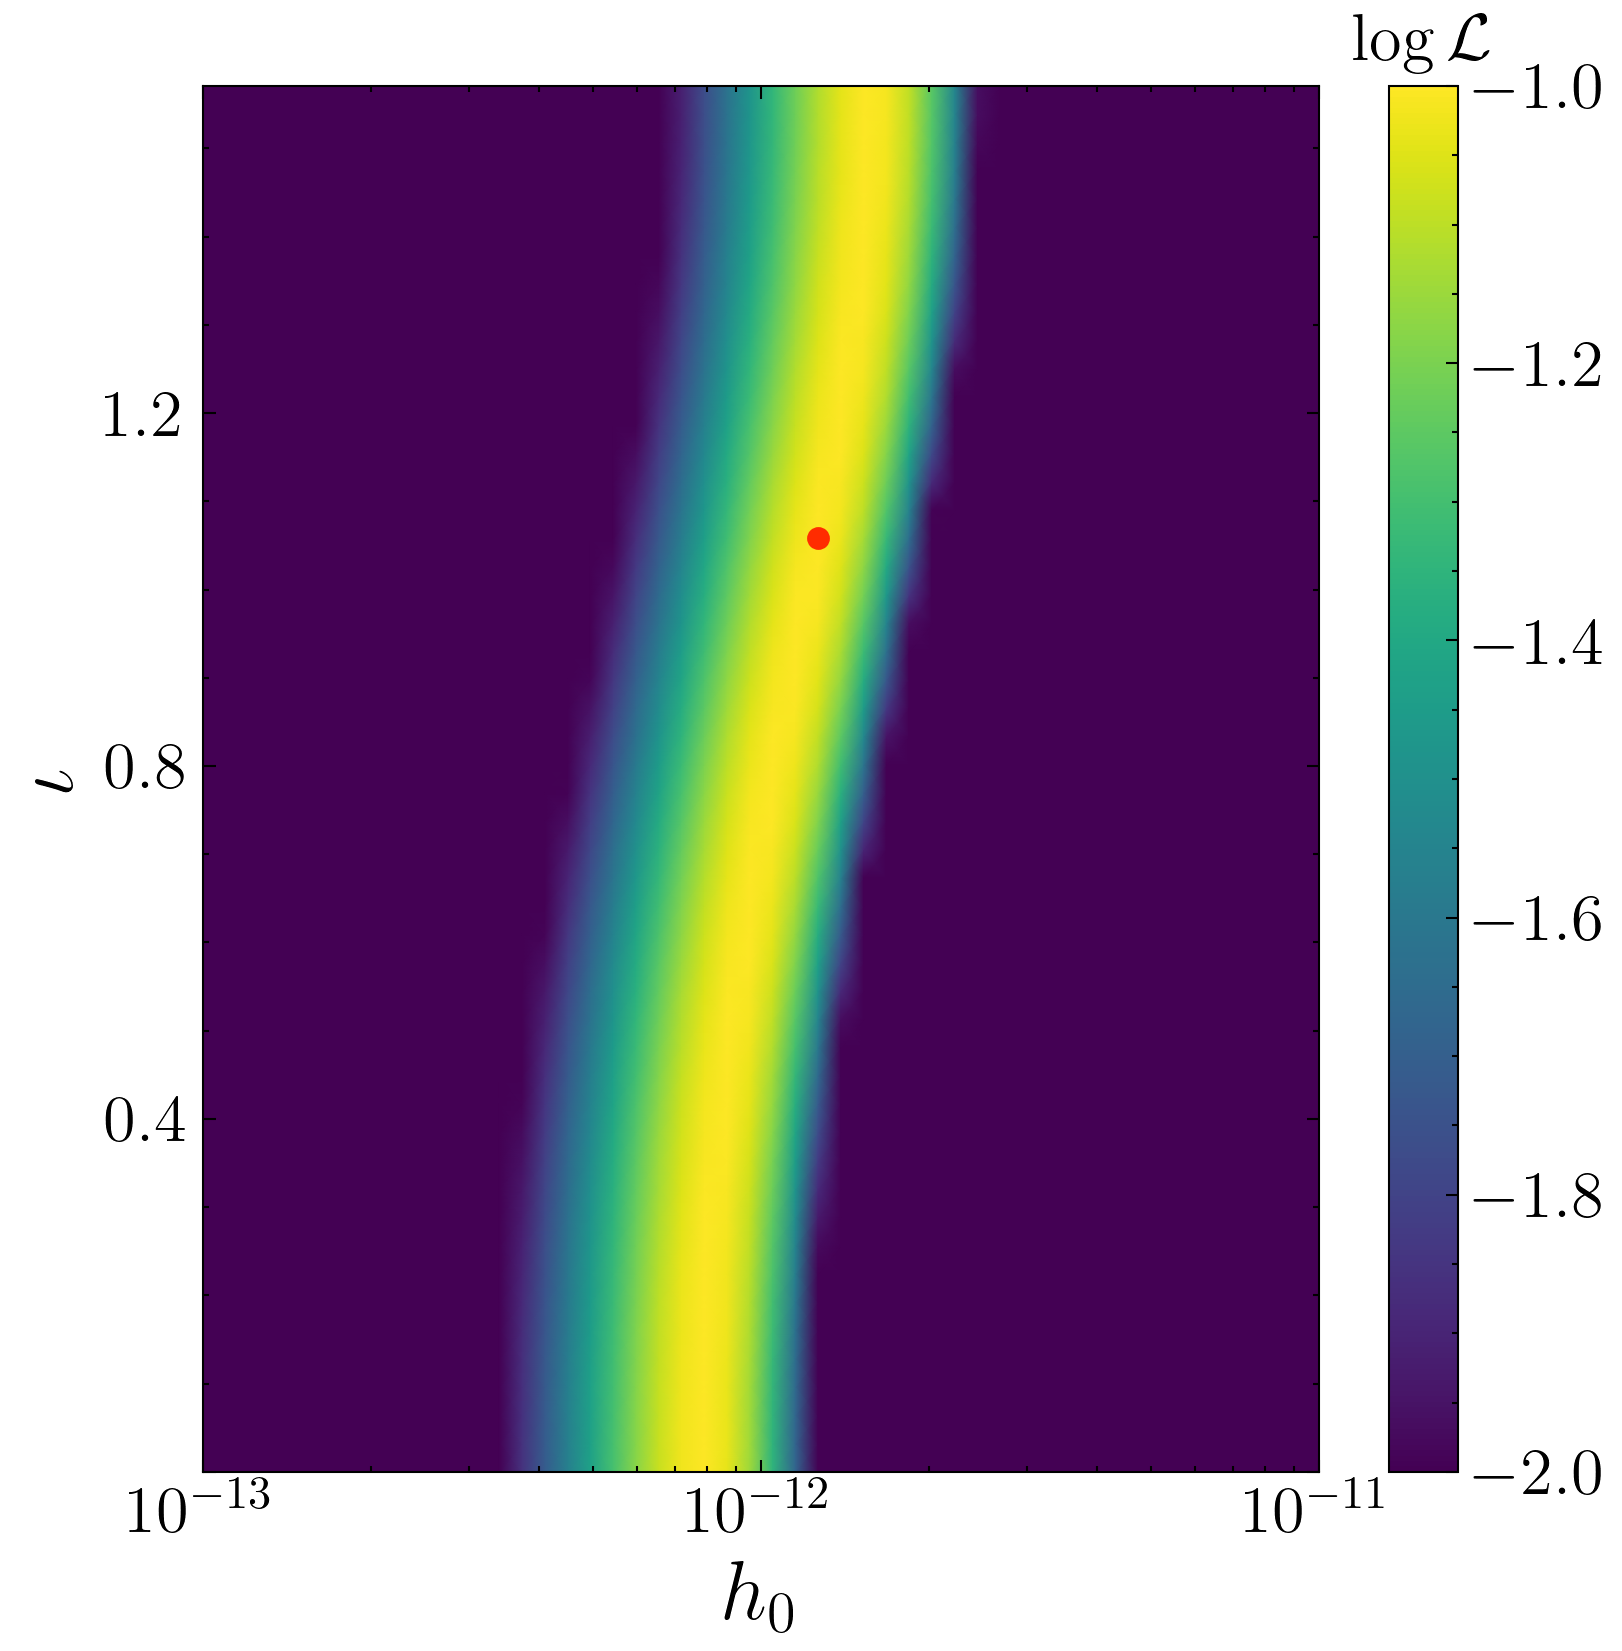
\includegraphics[width=\columnwidth]{images/likelihood_surface}
	\caption{Likelihood $\log \mathcal{L}$ (Equation \ref{eq:likelihood}) surface across the $\iota - h_0$ parameter space for a single noise realisation. The red point labels the location of the likelihood maxima. The likelihood surface has been normalised with respect to the absolute value of the maxima. A strong likelihood ridge is evident in the parameter space where the Kalman filter produces similar likelihood values, making it difficult for sampling algorithms to converge to a consistent value.}
	\label{fig:likelihood_surface}
\end{figure}
In Figure \ref{fig:just_iota_h} we plot the estimated one-dimensional posteriors for $\iota$ and $h_0$ for our high-SNR representative system, over nine noise realisations. 
The figure is entirely analogous to Figure \ref{fig:corner_plot_2}, but just for $\iota$ and $h_0$ rather than all members of $\boldsymbol{\theta}_{\rm gw}$. In the case of high-SNR we might expect \textit{a priori} that our estimates would be increasingly accurate over the low-SNR case, and that the method would converge robustly to similar posteriors irrespective of the noise realisation (i.e. $W_1 \to 0$). This is generally true for the majority of the component parameters of $\boldsymbol{\theta}_{\rm gw}$; the estimated posteriors across noise realisations are largely indistinguishable. However for $\iota$ and $h_0$ this is not the case. Instead the inferred one-dimensional posteriors do not broadly overlap and are not consistent across different noise realisations. Specifically across $10^3$ noise realisations the median WD for $\iota$ is $W_{1, \rm median}=0.24$ rad and for $h_0$ is  $W_{1, \rm median}=1.6 \times 10^{-13}$. For $\iota$, $W_{1,\rm median}$ is greater than the value inferred in the low SNR case ($=0.14$, Table \ref{tab:Wasserstein}), whilst for $h_0$ $W_{1,\rm median}$ is also greater as a proportion of the scale set by the strain amplitude. This is in contrast to $W_{1,\rm median}$ inferred for the other parameters of $\boldsymbol{\theta}_{\rm gw}$ in the high-SNR regime where as SNR increases, $W_1$ decreases; e.g. for $\Phi_0$, $W_{1, \rm median} = 4.5 \times 10^{-3}$ rad. \newline 

This issue of inferring very different posteriors depending on the particular realisation of the noise is due to these parameters being only weakly-identifiable. Identifiability refers to whether it is theoretically possible to infer unique parameter values of the model, given the measured data and the model structure \citep{e5be7c83a0d24500826f6e1b414d1733}. Sources of non-identifiability are generally categorised as either ``structural", arising from the structure of the model, or ``practical", arising from insufficient data or measurement errors \citep{GUILLAUME2019418}. Regarding $\iota$ and $h_0$, we are concerned with structural identifiability. Indeed, one might initially suspect that $\iota$ and $h_0$ could have structural identifiability issues; from Equations \eqref{eq:hphx} and \eqref{eq:hphx2} we can see that there is a weak degeneracy between $\iota$ and $h$. For example, from Equation \eqref{eq:hphx2} it is not clear if a larger value of the cross polarisation strain $h_{\times}$ is due to the system having a larger strain amplitude $h_0$, or a different inclination $\iota$. This degeneracy is only broken by the relation for $h_{+}$, Equation \eqref{eq:hphx}. It can be shown (Appendix \ref{appendix_identifiability}) that $\iota$ and $h_0$ are in fact structurally identifiable, but with the caveat that they are only weakly-identifiable. That is to say the $\iota-h_0$ likelihood surface plateaus to a ridge with a small, non-zero gradient close to the maximum likelihood solution. This likelihood ridge is presented in Figure \ref{fig:likelihood_surface} for a particular noise realisation. Whilst a single, unique maxima exists (labelled by the red point in the figure), along the ridge in the parameter space the likelihood values are all very similar. Consequently it is difficult for the nested sampling algorithm to select a particular point in this plateau and instead effectively trades off accuracy in one parameter against accuracy in other, depending on the particular realisation of the noise. If during the inference we fix one of the parameters at its true value (i.e. set a delta function prior), taking a slice through the likelihood surface it is then possible to identify a particular point in the plateau and the posteriors for the different noise realisations overlap indistinguishably, i.e. $W_1 \to 0$. In the low-SNR case these parameters are also weakly identifiable, but the increased measurement noise increases the uncertainty which effectively ``washes out" \footnote{\tiny \textcolor{red}{TK: "washes out" may be too colloquial / unspecific, but I think it is intuitive...}\normalsize}the likelihood ridge, leading to a more concave likelihood surface. This enables consistent posteriors to be estimated for $\iota$ and $h$. In the case where we fix e.g $h_0$ at its true value to infer indistinguishable posteriors for $\iota$, all of the posteriors for $\iota$ are all strongly biased away from the injected value; the maximum a posteriori probability estimates underestimate the injected value by $\sim 0.34$ rad. This is a more definitive sign of the bias that was suggested at in Sections \ref{sec:parameter_estim} and \ref{sec:multiple_noise} and will be now be discussed further in Section \ref{sec:bias}. 
\subsection{Bias by dropping pulsar terms}\label{sec:bias}

\begin{figure*}
	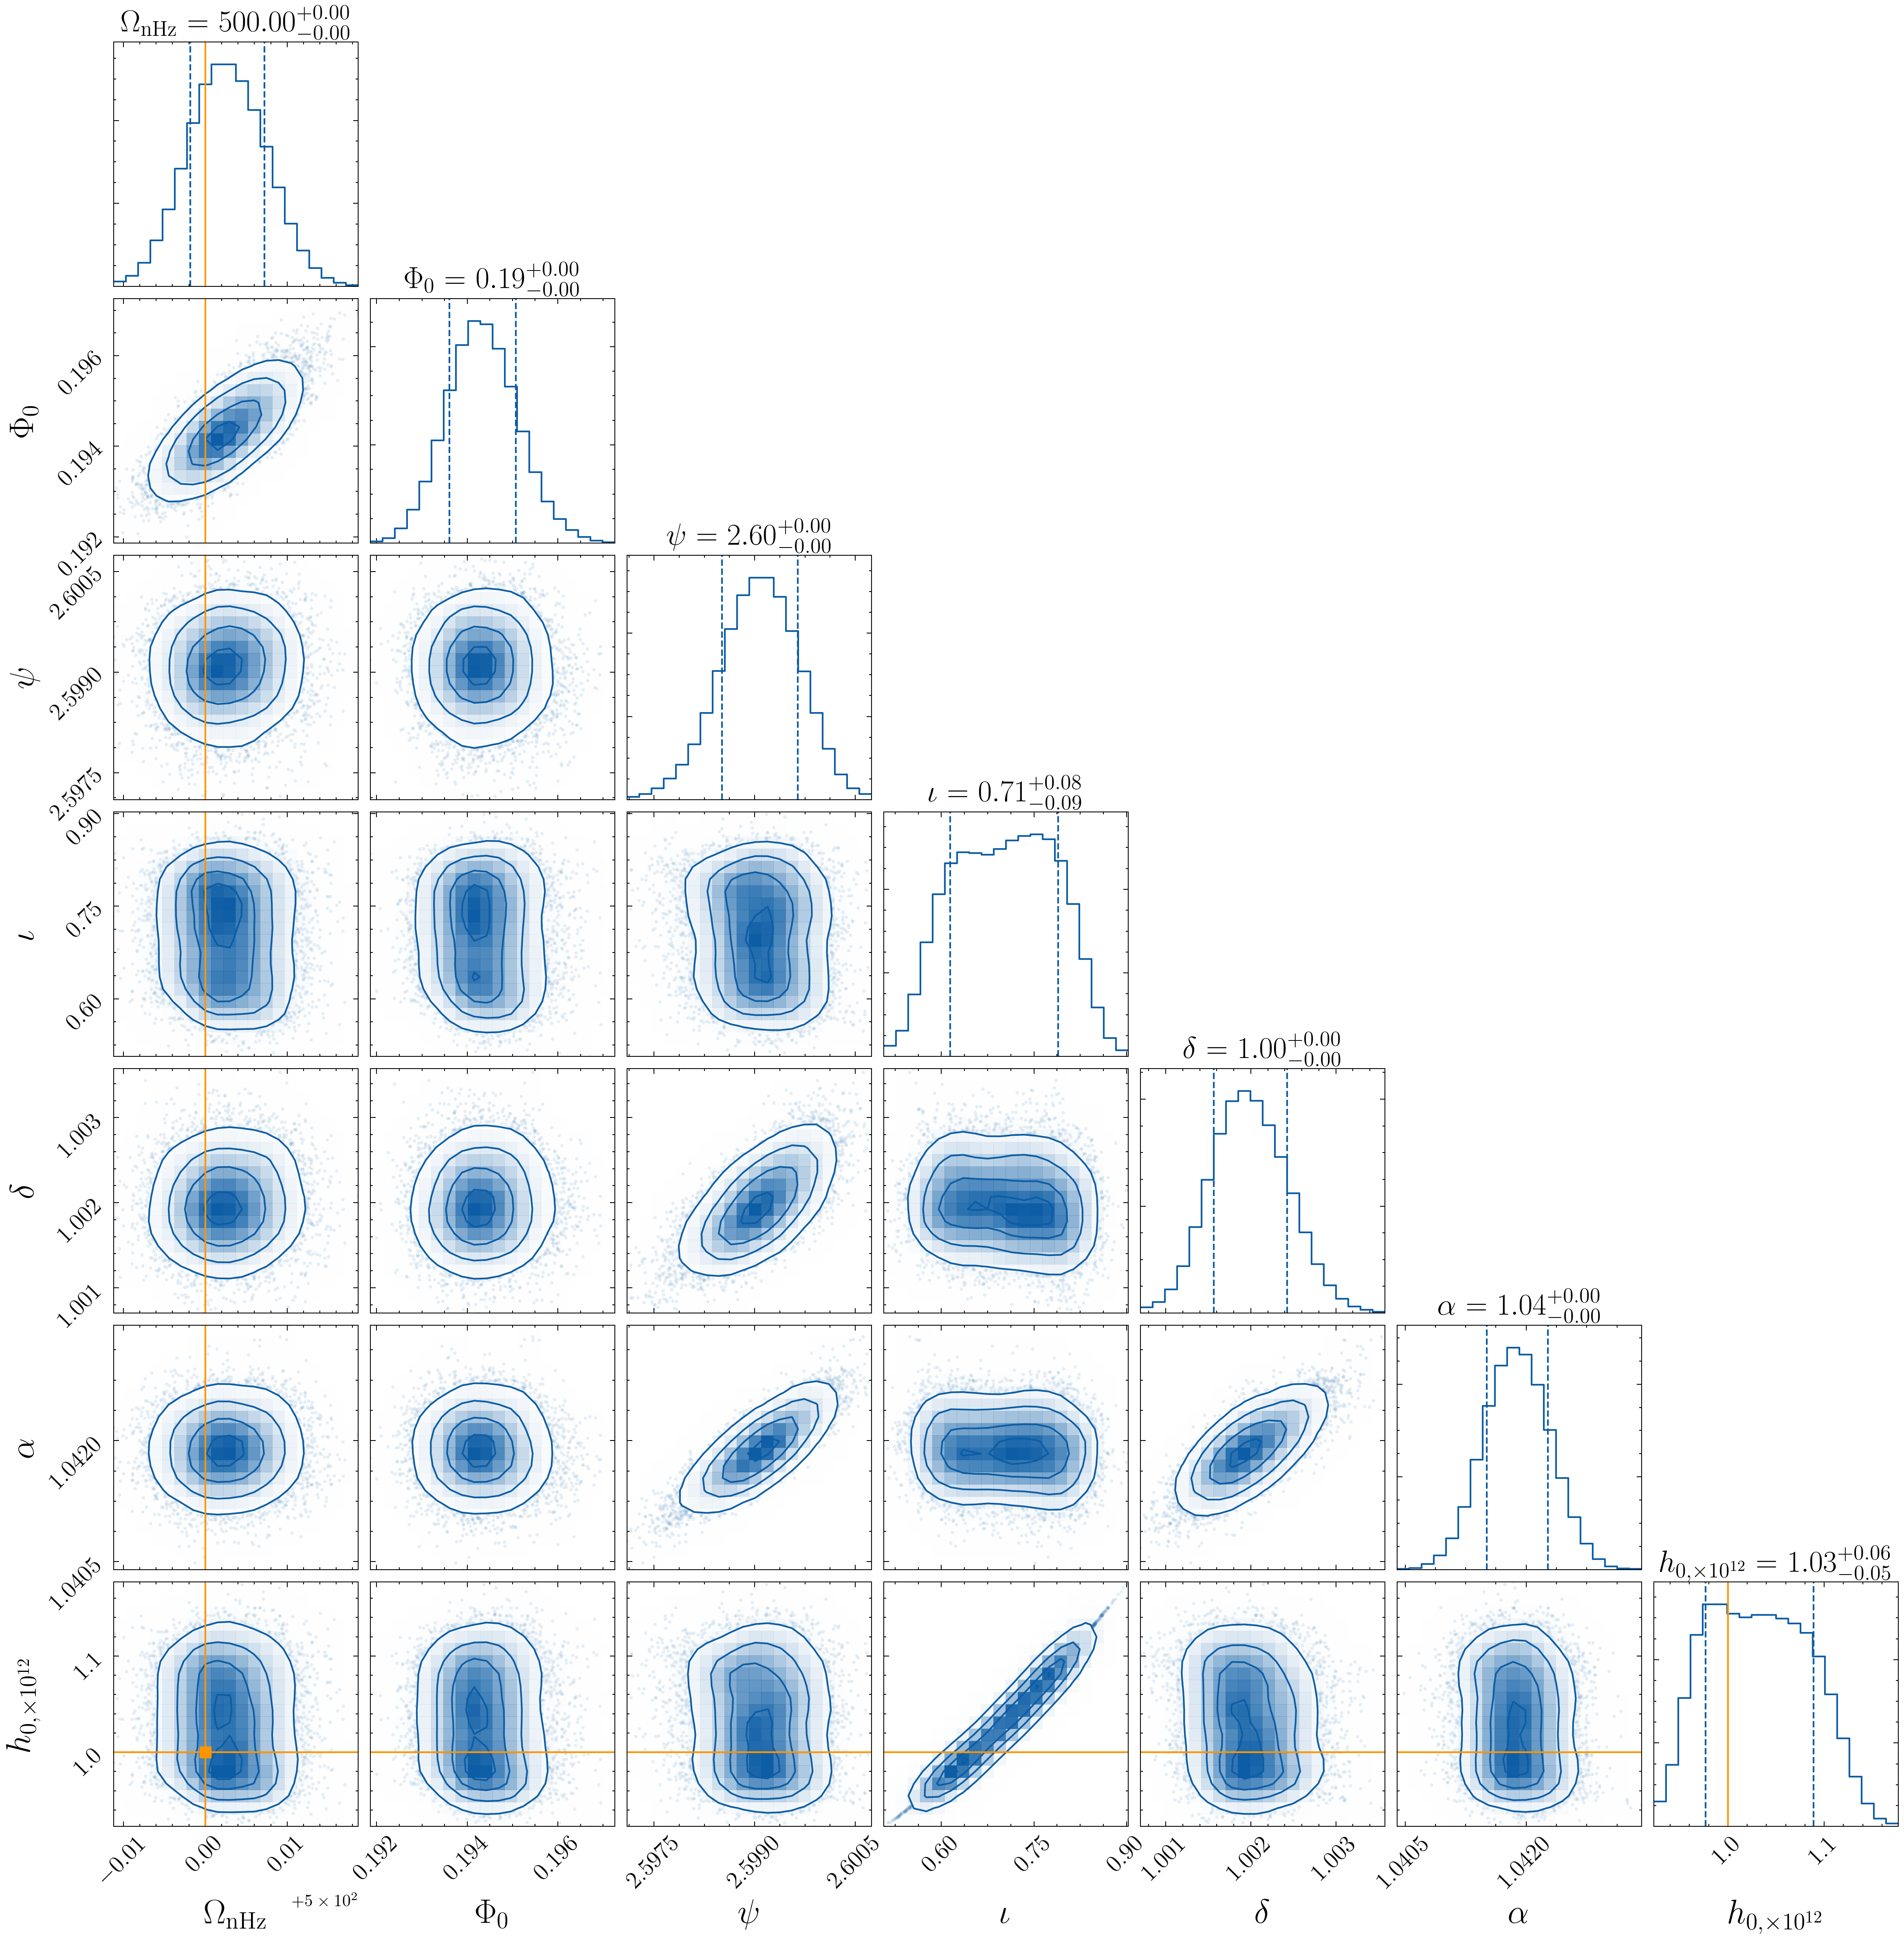
\includegraphics[width=\textwidth, height =\textwidth]{images/large_h_example}
	\caption{As Figure \ref{fig:corner_plot_1} but for the high-SNR system with $h_0 = 10^{-12}$. For the majority of parameters the injection value does not fall within the 90\% credible interval and is not visible over these scales. The estimated posteriors are biased away from the injected value due to the dropping of the pulsar terms. Note that the scale of the $x$-axes are generally highly constrained compared to Figure \ref{fig:corner_plot_1}.} 
	\label{fig:bias_for_large_h}
\end{figure*}

\begin{figure}
	\centering
	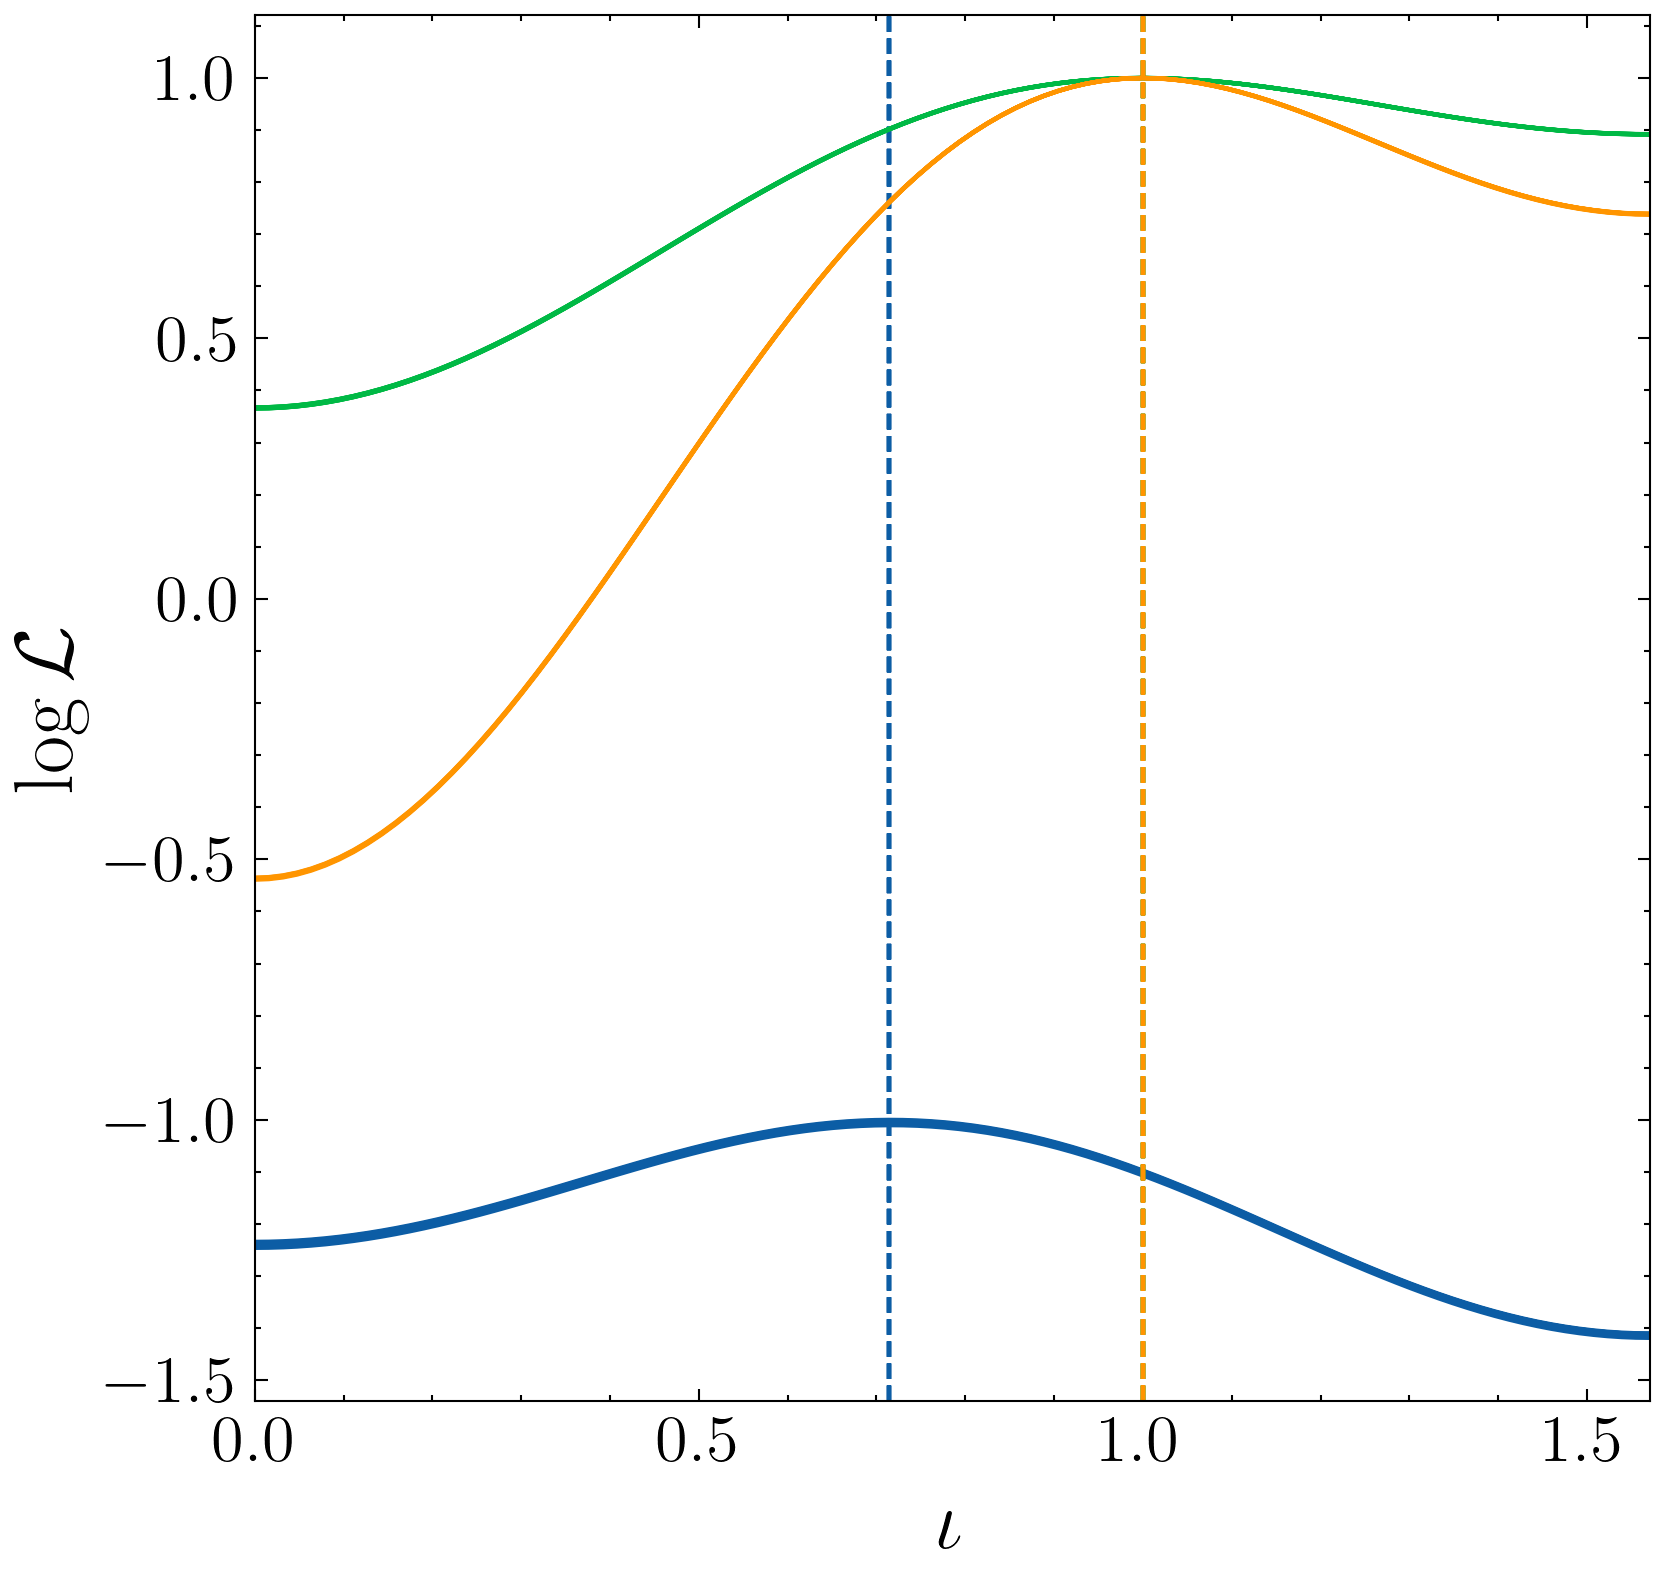
\includegraphics[width=\columnwidth]{images/likelihood_iota_new}
	\caption{Variation in the log likelihood returned by the Kalman filter using the Earth terms model (Equation \ref{eq:measuremen_earth}, blue line), the pulsar terms model (Equation \ref{eq:measurement}, orange line), and the Earth terms model for Earth terms only synthetic data (green line), with respect to the inclination $\iota$, over the prior space. All other parameters are fixed at their true injected value from Table \ref{tab:parameters_and_priors}. The coloured dashed vertical lines label the location of the likelihood maxima for their corresponding model; the green/orange dashed lines are overlaid on this scale. For the Earth-terms model the likelihood maxima does not coincide with the injected value ($\iota = 1.0$). For the pulsar-terms model the location of the maxima and injected value do coincide. 10 noise realisations are plotted for each situation but the solutions are completely overlaid on this scale.}
	\label{fig:likelihood_surface_iota}
\end{figure}
Evident in the preceding discussion is the fact that for some of the $\boldsymbol{\theta}_{\rm gw}$ parameters the inferred value (e.g. the median of the one-dimensional marginalised posterior) is biased away from the true injection value. In Figure \ref{fig:bias_for_large_h} we show the resulting posteriors for $\boldsymbol{\theta}_{\rm gw}$, analogous to Figure \ref{fig:corner_plot_1}, but now for the high-SNR system with $h_0 = 10^{-12}$. We can see that for all parameters, with the exception of $\Omega$ and $h_0$, the injected value lies outside the 90\% credible interval, to the extent that it is not visible on the scales over which we have plotted the posteriors. This effect is most severe for $\iota$ with a bias of $\sim 0.3$ rad but is also present to a lesser extent in other static parameters such as $\delta,\alpha$ and $\psi$, and additionally to an even smaller extent in $\Phi_0$. Similar results are obtained for other noise realisations. Whilst $h_0$ does not exhibit any noticeable bias for this particular noise realisation, in general across multiple noise realisations it does exhibit a correlated bias with $\iota$. In this Section we demonstrate how this bias results from the dropping of the pulsar terms described in Section \ref{sec:parameter_estim}. \newline 


In Figure \ref{fig:likelihood_surface_iota} we plot the variation in the log-likelihood returned by the Kalman filter, Equation \eqref{eq:likelihood}, as we vary $\iota$ across the prior space, holding all other parameters constant at the true injected value of the representative example system, Table \ref{tab:parameters_and_priors}. We do this for 10 separate realisations of the system noise. We consider three separate situations: \textit{(i)} The solid blue line is the likelihood curve with just the Earth-terms included (i.e. using Equation \ref{eq:measuremen_earth} in the Kalman filter), \textit{(ii)} the solid orange line is the likelihood curve with the additional pulsar terms included (i.e. using Equation \ref{eq:measurement}), \textit{(iii)} the solid green line is the solution where we drop the pulsar terms from both the synthetic data and the measurement equation. We have not used nested sampling for situations \textit{(ii)} or \textit{(iii)} in this work. However, we are able to run the Kalman filter either using the pulsar terms in the model or else dropping them from the synthetic data consider how the resulting likelihood varies for different parameter values. The dashed lines show the location of the likelihood maxima for each of the likelihood solutions; finding the location of the maxima across all static parameters is effectively the goal of any likelihood based inference method, such as nested sampling. \newline  

The key observation from Figure \ref{fig:likelihood_surface_iota} is that for the Earth-terms only solution the location of the likelihood optima and the location of the injected value are not the same. Consequently Bayesian likelihood inference techniques settle in optima that do not necessarily align with the true injection value. This is the origin of the bias in the one-dimensional marginalised posteriors that we observe.  For the Earth-terms solution the optima of the likelihood curve lies around $\iota \sim 0.7$ rad, whereas the injected value was $\iota = 1.0$ rad. This optima is comparable to the median of the posterior inferred for $\iota$ in Figure \ref{fig:bias_for_large_h}. \newline 

In contrast to the Earth-terms solution, for the pulsar-terms solution the optima of the likelihood curve now aligns with the true injected value. The corollary is also true; if we drop the pulsar terms from the synthetic data and use the Earth terms equation for inference then the optima is also correctly located. This evidences that it is the effect of dropping the pulsar terms from the measurement equation which causes this bias in the inferred posteriors. Similar results are observed for the other parameters which exhibit a bias in the nested sampling inference. \newline 

Why does dropping the pulsar terms bias these parameters in particular, whilst leaving others unaffected? For instance, why is the bias induced in $\iota$ so strong, whereas $\psi$ shows only a weak bias and  $\Omega$ shows no bias at all? When we generate synthetic data including the pulsar term, the state frequency of an individual pulsar $f_{\rm p}$ is effective modulated by the interference of two equal-amplitude, phase shifted waves (c.f. Equation \ref{eq:measurement}). Explicitly, we have the ``Earth-terms wave"	 with a general form $y_{\rm Earth} = A \cos \xi$ for amplitude $A$ and phase $\xi$ and the ``pulsar-terms wave" with a general form $y_{\rm pulsar} = A \cos (\xi + \kappa)$ for phase offset $\kappa$. The net interference wave that modulates $f_{\rm p}$ is 
\begin{eqnarray}
	y_{\rm Earth} - y_{\rm pulsar} = 2 A \sin \left(\frac{\kappa}{2}\right) \sin \left(\xi + \frac{\kappa}{2}\right) \ .
\end{eqnarray}
The additional modulations from $y_{\rm pulsar}$ influence the amplitude of the resulting interference wave, but do not affect its frequency. When we model this data using the Kalman filter without the pulsar terms, the additional amplitude modulations from $y_{\rm pulsar}$ must be described by the single wave model, $y_{\rm Earth}$. As a result the $y_{\rm Earth}$ model must try to compensate for these amplitude modulations by adjusting the parameters which govern the amplitude of the single wave. Consequently the parameters which are most affected are those which determine the amplitude of the GW. Terms which influence the amplitude strongly, such as $h_0$ and $\iota$, are strongly affected and exhibit a strong bias. Terms which influence the amplitude weakly such as $\psi$ exhibit a weaker bias. The wave amplitude is independent of the frequency and so $\Omega$ exhibits no bias. Since a shift in phase affects the instantaneous amplitude of the wave, $\Phi_0$ also exhibits a small bias, despite $A$ not being a function of $\Phi_0$. This hierarchy of biases for each parameter is also what we observe in Figure \ref{fig:parameter_space}, where $\alpha$ and $\delta$ are strongly over-constrained whilst $\Omega$ is well-estimated. \newline  

In order to ascertain how important the bias is for PTA continuous wave searches requires a thorough exploration of the astrophysical parameter space which we do not carry out in this work. The magnitude of the bias will vary for different points in the parameter space, as well as for different PTA configurations. If the bias is sufficiently modest then for quiet continuous wave sources with low SNR the uncertainty in the one-dimensional marginalised posterior may dominate and the bias may not be important for searches. This is what we observe for our synthetic data (e.g. Figure \ref{fig:corner_plot_2}); the decreased SNR manifests as a broader marginalised posterior which generally overwhelms the shift due to the bias. Conversely if the bias is sufficiently strong, or the source sufficiently loud with low uncertainties, then the bias may come to systematically affect the inferred parameters. \newline  

We have shown in this section how the dropping of the pulsar terms results in a bias in the inferred parameters, not just in the sky localisation parameters  \citep[e.g.][]{Zhupulsarterms,Chen2022} but additionally all parameters which influence the wave amplitude. Whilst the bias is generally small and does not prevent the recovery of accurate posteriors for our example system, it is present and may need to be accounted for for analysis in other parts of the parameter space. This bias is not particular to our method but a shared feature across likelihood based methods that do not include the pulsar terms in the inference model. The inclusion of the pulsar terms in the methods presented in this work in order to alleviate the bias will be a key goal of a future work. 


\section{Discussion}\label{sec:discussion}
We have shown how our complementary approach to PTA data analysis using a Kalman filter can successfully recover the underlying parameters of the model and calculate Bayes factors in order to perform Bayesian model selection. There are a number of potential extensions of this work which we now discuss.  \newline 

The natural first extension is to implement the method whilst retaining the pulsar terms of Equation \ref{eq:measurement}. Whilst PTA searches commonly drop the pulsar terms as standard practice, we have shown that this leads to biases in the inferred one-dimensional marginalized posteriors for the model parameters. Biases in sky localisation for synthetic datasets as a result of dropping the pulsar terms are also observed by \cite{Zhupulsarterms} and \cite{Chen2022}. Alternatively, if the method continues to be used with solely the Earth terms then it would be highly desirable to make systematic, quantitative estimates of the incurred biases in the model parameters across an astrophysically representative parameter space. \newline 

We have considered only a specific configuration of pulsars composing our synthetic PTA - the same pulsars that make up the 12.5-year NANOGrav (Section \ref{sec:synt_pta}). Whilst our method is generally independent of the specific choice of pulsars, it would be of interest to compare the performance of the method using different pulsars configurations and different PTAs such as PPTA and the EPTA. Indeed, since adding pulsars to PTAs increases the computational demands of the data analysis it may be advantageous to optimally select a subset of the total available pulsars which may be able to provide comparable performance to a larger PTA  \citep{2023MNRAS.518.1802S}.  \newline 

Throughout this work we have assumed that all pulsars are observed at the same time, with a constant time sampling. In practice this assumption does not hold and different pulsars will be observed with different cadences at different times. Extending this method to non-constant time sampling is straightforward and the performance of the method should be evaluated in this regime. \newline 

We have taken our GW source to be monochromatic, i.e. $\Omega$ is a fixed parameter with no time dependence. Whilst this is an astronomically well-justified assumption (see discussion in Section \ref{sec:plane_gw}), and appropriate for this initial methods work, it would also be of interest to extend the state-space construction to enable the GW frequency to evolve in time. The GW source is monochromatic over the decadal PTA observation period, but the timescale set by the Earth-pulsar distance is comparable to the SMBHB evolution timescale \citep{Sesana2010}. For $\Delta f_{\rm gw} < 1 / T_{\rm obs}$ (see Equation \eqref{eq:f_evolution}) the GW source frequency evolution manifests as an incoherent source of noise in the pulsar terms, whilst for  $\Delta f_{\rm gw} > 1 / T_{\rm obs}$ the pulsar terms can affect the phase coherency of the Earth terms \citep{Perrodin2018}. Careful consideration of the evolution of the GW frequency will be important as we look to extend our method to include the pulsar terms in the inference model. \newline 


We have also assumed that there is only a single GW source that influences the received pulsar frequencies. However, it may be possible to resolve multiple continuous GW sources concurrently \citep{PhysRevD.85.044034}. Our method naturally extends to detecting multiple GW sources simultaneously; Equation \eqref{eq:measurement} is straightforwardly modified to become a linear superposition of multiple GWs. The stochastic background itself is the incoherent summation of many individual GW sources. It therefore stands to reason that it may be possible to extend this method to also search for a stochastic GW background, providing a complementary approach to detect the stochastic background without requiring a cross-correlation of the pulsar residuals to uncover the Hellings-Downs curve. \newline 


\textcolor{red}{TK: Lets also pre-empt reviewer and make it explicit why we are using frequencies rather than TOAs. Need to chat with group to get this clear in my head.}


%https://arxiv.org/pdf/2107.03047.pdf
\section{Conclusion}\label{sec:conclusion}
In this paper we demonstrate a new method for the detection and parameter estimation of GWs from individual, monochromatic SMBHBs. We track the evolution of the intrinsic pulsar timing noise explicitly via a state-space method, rather than subtracting the ensemble-averaged statistics. That is, we disentangle statistically the specific time-ordered realisation of the timing noise from the GW induced modulations. This enables the inference of GW parameters conditioned on the specific observed realisation of the noisy data. We introduce the Kalman filter in order to track the intrinsic state evolution of the pulsar and combine this with a Bayesian sampling framework to estimate the posterior distributions of each parameter of the system, as well as the associated evidence (marginalised likelihood) of the model. We test our method on synthetic data. We initially focus on a single, astrophysically representative, SMBHB GW source detected with the 12.5-year NANOGrav pulsars observed over a 10 year timespan. The parameters of the model are accurately recovered and the minimal detectable strain is estimated to be $h_0 \sim 4 \times 10^{-15}$ for $\iota=1.0$ rad. The method is then further tested over 1000 noise realisations. Consistent posterior estimates of the parameters are obtained for the majority of noise realisations, with the median Wasserstein distance across all noise realisations $W_{1, \rm median}$ generally small compared to the prior space ($\lesssim 3 \%$). For a minority of noise realisations the nested sampler converges poorly and settles into a local likelihood optima for the posteriors estimates of $\psi$ and $\alpha$. This problem can be solved in general by increasing the number of live points $n_{\rm live}$ used by the sampler. Exploration of a broader parameter space via 200 randomly sampled parameter vectors highlights biases in some parameters as a result of dropping the pulsar terms from the inference model. The cause of these biases is examined for the case of high SNR, along with the structural weak-identifiability between $\iota$ and $h_0$. The extension of this method to include the pulsar term is a key challenge for a future work.
 
 

 
\appendix

\section{Kalman recursion equations} \label{sec:kalman}
The linear Kalman filter operates on temporally discrete, noisy measurements $\boldsymbol{Y}_k$, which are related to a set of unobservable discrete system states $\boldsymbol{X}_k$, via a linear transformation:
\begin{equation}
	\boldsymbol{Y}_k = \boldsymbol{H}_k \boldsymbol{X}_k + \boldsymbol{v}_k \ ,\label{eq:kalman1}
\end{equation}
where $\boldsymbol{H}_k$ is the measurement matrix or observation model, $\boldsymbol{v}_k$ is a zero-mean Gaussian measurement noise, $\mathcal{N} \sim (0,\boldsymbol{R}_k)$ with covariance, and the subscript $k$ labels the time-step. The Kalman filter takes the underlying states to evolve according to
\begin{equation}
	\boldsymbol{X}_k = \boldsymbol{F}_k \boldsymbol{X}_{k-1} + \boldsymbol{G}_k \boldsymbol{u}_k + \boldsymbol{w}_k \ , \label{eq:kalman2}
\end{equation}
where $\boldsymbol{F}$ is the system dynamics matrix, $\boldsymbol{G}$ the control matrix. $\boldsymbol{u}$ the control vector, and $\boldsymbol{w}_k$ is a zero-mean Gaussian process noise, $\mathcal{N} \sim (0,\boldsymbol{Q}_k)$. \newline 

The Kalman filter is a recursive estimator with two distinct stages; a ``predict" stage and an ``update" stage. The predict stage predicts the estimate of the state at discrete step $k$, given the state estimates from step $k-1$. Specifically, the predict step proceeds as,
\begin{equation}
	\hat{\boldsymbol{X}}_{k|k-1} =  \boldsymbol{F}_k \hat{\boldsymbol{X}}_{k-1|k-1} + \boldsymbol{G}_k \boldsymbol{u}_k
\end{equation}
\begin{equation}
	\hat{\boldsymbol{P}}_{k|k-1} =  \boldsymbol{F}_k \hat{\boldsymbol{P}}_{k-1|k-1} \boldsymbol{F}_k^\intercal + \boldsymbol{Q}_k 
\end{equation}
Note that the predict stage is independent of the measurements. The measurement $\boldsymbol{Y}_k$ is included to update the prediction during the update stage as follows:
\begin{equation}
	\boldsymbol{\epsilon}_{k} = \boldsymbol{Y}_k - \boldsymbol{H}_k \hat{\boldsymbol{X}}_{k|k-1}
\end{equation} 
\begin{equation}
	\boldsymbol{S}_k = \boldsymbol{H}_k \hat{\boldsymbol{P}}_{k|k-1} \boldsymbol{H}_k^\intercal + \boldsymbol{R}_k
\end{equation}
\begin{equation}
	\boldsymbol{K}_k = \hat{\boldsymbol{P}}_{k|k-1} \boldsymbol{H}_k^\intercal \boldsymbol{S}_k^{-1} \label{eq:kalman gain}
\end{equation}
\begin{equation}
	\hat{\boldsymbol{X}}_{k|k} =\hat{\boldsymbol{X}}_{k|k-1} +\boldsymbol{K}_k  \boldsymbol{\epsilon}_{k}  \label{eq:kalmangainupdate}
\end{equation}
\begin{equation}
		\hat{\boldsymbol{P}}_{k|k} = \left( \boldsymbol{I} - \boldsymbol{K}_k \boldsymbol{H}_k \right) 	\hat{\boldsymbol{P}}_{k|k-1}
\end{equation}
Equation \eqref{eq:kalman gain} defines the ``Kalman gain" $\boldsymbol{K}_k$ which is defined so as to minimise the mean squared error in the state estimate, i.e.  $\boldsymbol{K}_k = \text{argmin} \left[ \boldsymbol{E}(\boldsymbol{X}_k - \hat{\boldsymbol{X}}_k) \right ]$. For a full review of the Kalman filter, including its derivation, we refer the reader to \cite{Gelb:1974} and \cite{zarchan2000fundamentals}. \newline 


We map our continuous-time state-space model described in Section \ref{sec:model} onto the discrete-time Kalman filter structure of Equations  
\eqref{eq:kalman1}, \eqref{eq:kalman2} as follows. We identify $\boldsymbol{X}$ with a vector of length $N$ composed of the intrinsic pulsar frequency states, i.e 
\begin{equation}
	\boldsymbol{X} = \left(f_{\rm p}^{(1)}, f_{\rm p}^{(2)}, ..., f_{\rm p}^{(N)}\right) \ .
\end{equation}
Similarly,  
\begin{equation}
\boldsymbol{Y} = \left(f_{\rm m}^{(1)}, f_{\rm m}^{(2)}, ..., f_{\rm m}^{(N)} \right)
\end{equation}
The states evolve according the continuous dynamical equation (c.f. Equation \eqref{eq:frequency_evolution})
\begin{equation}
	d \boldsymbol{X} = \boldsymbol{A} \boldsymbol{X} dt + \boldsymbol{C}(t) dt + \boldsymbol{\Sigma} d \boldsymbol{B}(t) \label{eq:kalmn2}
\end{equation}
where $\boldsymbol{A}$ is a diagonal $N \times N$ square matrix
\begin{equation}
\boldsymbol{A} = \text{diag} \left(\gamma^{(1)}, \gamma^{(2)}, ..., \gamma^{(N)}\right) \ ,
\end{equation}
and $\boldsymbol{C}(t)$ a time dependent vector with $n$-th component
\begin{equation}
 C^{(n)} =\gamma^{(n)} \left(f_{\rm em}^{(n)} (t_1) + \dot{f}_{\rm em}(t_1)^{(n)} t \right) +  \dot{f}_{\rm em}(t_1)^{(n)} \ .
\end{equation}
The $N \times N$ square matrix $\boldsymbol{\Sigma}$  governs the magnitude of the increments of Brownian motion (Wiener process) $d\boldsymbol{B}(t)$, where
\begin{equation}
\boldsymbol{\Sigma} = \text{diag} \left(\sigma^{(1)}, \sigma^{(2)}, ..., \sigma^{(N)}\right)
\end{equation}
\newline 

The evolution of the state is an Ornstein-Uhlenbeck process, described by a Langevin equation, Equation \eqref{eq:kalmn2}, which has a general solution given by \citep{gardiner2009stochastic},
\begin{equation}
	\boldsymbol{X}(t) = e^{\boldsymbol{A} t} \boldsymbol{X}(0) + \int_0^t e^{\boldsymbol{A}(t-t')} \boldsymbol{C}(t') dt' + \int_0^t e^{\boldsymbol{A}(t-t')} \boldsymbol{\Sigma} d\boldsymbol{B}(t') \label{eq:gardenier}
\end{equation} 
From Equation \eqref{eq:gardenier} we can construct the discrete, recursive solution for $\boldsymbol{X}(t_k) = \boldsymbol{X}_k$ in the form of Equation \eqref{eq:kalman2} where
\begin{equation}
\boldsymbol{F}_k = e^{\boldsymbol{A}\left( t_{k+1} - t_k \right)} 
\end{equation}
\begin{equation}
	\boldsymbol{G}_k = \int_{t_i}^{t_{i+1}}  e^{\boldsymbol{A}\left( t_{k+1} - t' \right)}  \boldsymbol{C}(t') dt' 
\end{equation}
\begin{equation}
	\boldsymbol{w}_k = \int_{t_k}^{t_{k+1}} e^{\boldsymbol{A}\left( t_{k+1} - t' \right)} \boldsymbol{\Sigma} d \boldsymbol{B}(t')
	\end{equation}
For our system, the state, control and process noise covariance matrices then take the form:
\begin{equation}
	\boldsymbol{F}_k = 	\text{diag}\left(e^{- \gamma^{(1)} \Delta t},e^{- \gamma^{(2)} \Delta t},...,e^{- \gamma^{(N)} \Delta t} \right)
\end{equation}
\begin{equation}
\boldsymbol{G}_k	= \left(G^{(1)}_k, G^{(2)}_k,...,G^{(N)}_k \right)
\end{equation}
with
\begin{align}
	G_k^{(n)} =&    f^{(n)}_{\rm em}(t_1) + \dot{f}^{(n)}_{\rm em}(t_1)  \left[\Delta t + t_k \right] \nonumber \\ 
	&- e^{-\gamma \Delta t} \left[  f^{(n)}_{\rm em}(t_1) +\dot{f}^{(n)}_{\rm em}(t_1)  t_k \right]
\end{align}
and
\begin{equation}
	\boldsymbol{Q}_k \boldsymbol{\delta}_{kj}= \langle \boldsymbol{\eta}_k \boldsymbol{\eta}_j^\intercal \rangle = \text{diag} \left(Q^{(1)}, Q^{(2)},...,Q^{(N)}\right) 
\end{equation}
for 
\begin{equation}
	Q^{(n)} = \frac{- [\sigma^{n}]^2}{2 \gamma^{(n)}} \left( e^{-2 \gamma^{(n)} \Delta t} -1\right)
\end{equation}
where $\Delta t$ is the constant time sampling interval $=t_{k+1} -t_{k}$. \newline 

The remaining component matrices of the Kalman filter that we have not yet specified are the measurement matrix $\boldsymbol{H}_k$ and the measurement covariance matrix $\boldsymbol{R}_k$. These are defined straightforwardly from Equation \eqref{eq:measurement}. Specifically, 
$\boldsymbol{H}_k$ is a diagonal matrix where the $n$-th component of the diagonal is given by $g^{(n)}(t_k)$ from Equation \eqref{eq:g_func}. The measurement covariance $\boldsymbol{R}_k = E \left[ \boldsymbol{v} \boldsymbol{v}^\intercal \right] = \sigma^2_{\rm m}$.



\section{Fiducial pulsar values}\label{appendix_fiducial}
\textcolor{red}{TK: Do we really need this? The argument is for reproducibility, but we have a nice github repo that holds all the data we actually used, jupyter notebooks that show how the calculations are done. Perhaps it is sufficient to point the reader to the repo... } 
\section{Identifiability}\label{appendix_identifiability}
\textcolor{red}{TK TBD. An example calculation for a simple system using the methods of e.g. } \citep{KARLSSON2012941} \citep{SEDOGLAVIC2002735}



\section{Wasserstein distance}\label{sec:wasserstein}
The Wasserstein distance is a metric that defines a distance between two probability distributions $\mu(x)$ and $\nu(x)$. It has an intuitive interpretation as the lowest total cost with which one can move probability mass from $\mu$ to $\nu$, with respect to a cost function $c(x,y)$. For this reason it is sometimes known as the "Earth mover's distance". The $p$-th order Wasserstein distance between two distributions is
\begin{eqnarray}
	W_p(\mu,\nu)= \left( \inf_{\gamma \in \Gamma(\mu, \nu)}  \int c(x,y)^p d \lambda (x,y)\right)^{1/p} \label{eq:wasserstein} \ ,
\end{eqnarray}
where $p \in [1,\infty)$, $\lambda(x,y)$ is the transport plan, and $\Gamma(\mu, \nu)$ is the set of all joint probability distributions for $(x,y)$ that have marginals $\mu$ and $\nu$, i.e. $\Gamma(\mu, \nu)$ is the set of couplings of $\mu$ and $\nu$. 

The cost function can be freely chosen for the nature of the problem, but is commonly taken to be the absolute value function, $c(x,y) = |x-y|$, and we adopt the same cost function in this work. Given this choice of $c(x,y)$, for an empirical distribution $\hat{\mu}_n$ composed of $n$ i.i.d samples drawn from the underlying probability distribution $\mu$, the solution to the discrete form of Equation \eqref{eq:wasserstein} can be computed generally by the Hungarian algorithm \citep{Kuhn} in polynomial time $\mathcal{O}(n^3)$ \citep{Villani2009}. However, for $\mu$ defined on $\mathbb{R}^d$ it is well-known \citep{Dudley} that the Wasserstein distance suffers from the curse of dimensionality for dimensions $d \geq 3$:
\begin{eqnarray}
	\boldsymbol{E} [W_1(\hat{\mu}_n,\mu)] \asymp n^{-\frac{1}{d}} \ .
\end{eqnarray}
In order to circumvent this issue, in this work we calculate the Wasserstein distance exclusively between the one-dimensional marginalized posteriors, i.e. setting $d=1$. In this case Equation \eqref{eq:wasserstein} has a convenient, easily computed, closed form:
\begin{eqnarray}
	W_p(\mu,\nu)= \left(\int_0^1  F_{\mu}^{-1} (z) - F_{\nu}^{-1} (z) dz \right)^{1/p} \, \label{eq:wasserstein}
\end{eqnarray}
where $F_{\mu}(z)$ is the cumulative distribution function of $\mu$. \newline  


The use of the Wasserstein distance over more common probability measures such as the Kullback–Leibler divergence or the  Kolmogorov-Smirnoff test has a number of advantages. Firstly, it is intuitive, being the minimal amount of work required to transform one distribution into another. It also inherits the units of the underlying distributions, providing a convenient heuristic; if $W_1 =1$ between a pair of distributions with units e.g. radians then we can interpret this as the cost to transform between the two distributions is 1 radian. Further interpretability is provided by the Monge-Kantorovich duality \citep{villani2003topics,Villani2009}:
\begin{eqnarray}
	| \boldsymbol{E}(X_{\mu} )-\boldsymbol{E}(Y_{\nu} ) | \leq W_1(\mu, \nu) \ , \label{eq:WDdefn}
\end{eqnarray}
where $X_{\mu}$ and $Y_{\nu}$ are random variables of the distributions $\mu$ and $\nu$ respectively, and $\boldsymbol{E}$ denotes the expected value. That is, if $W_1 =1$ then the difference in the expected value of two random variables drawn from the two distributions is less than 1 radian. Secondly it is a versatile, non-parametric measure that requires no specific properties of the probability distributions that are being compared such as e.g. Gaussianity. Any two distributions can be compared, irregardless of whether they are continuous, discrete, singular or defined on different metric spaces. Thirdly, it is a true distance metric and as such satisfies desirable properties of a measure of distance such as symmetry and the triangle inequality. It also respects the geometry of the underlying metric space over which the distributions are defined. \newline   


For each parameter in $\boldsymbol{\theta}_{\rm gw}$ we calculate $W_1$ between every pair of posteriors across our $10^3$ noise realisations. The results are presented in Figure \ref{fig:pairwise_wasserstein}. The figure shows a lower triangular heat-map where each point denotes the $W_1$ value between a pair of posteriors. Small values of $W_1$ are magenta moving to red for large values of $W_1$. Note that the heat-map colour scaling is not the same for all subplots of the figure. It is evident that $W_1$ is generally small across all pairs of posteriors. We define $W_{1, \rm median}$ as the median value of $W_1$ across all $10^3 \choose 2$ pairs of noise realisations. The values of $W_{1, \rm median}$ for each parameter are quoted in Table \ref{tab:Wasserstein}. As a percentage of the width of the prior space (e.g. for $\alpha$ the width of the prior is $2 \pi$), the median $W_1$ for each parameter is $\lesssim 3 \%$. Generally speaking, the method converges to consistent one-dimensional posteriors for each parameter across different noise realisations. \newline


There are a small fraction of the total number of noise realisations which have a large Wasserstein distance from all the other posteriors of all the other noise realisations. These are the strong yellow lines in Figure \ref{fig:pairwise_wasserstein}. These correspond exclusively to posteriors which have converged poorly and not found the likelihood global maximum. For instance, the top strong horizontal yellow line in Figure \ref{figWD_psi}, which is identified by an asterisk in the figure, corresponds to a posterior for $\psi$ which has converged sub-optimally, with an estimated value of $\psi = 1.01 \pm 0.06$ rad, highly diverged from the true injected value of $2.50$ rad. The $W_1$ value between this posterior and all the posteriors inferred for all other noise realisations is $\sim 1.7$ rad. We also observe a strong correlation across all noise pairs (Pearson correlation coefficient $=0.96$) between the $W_1$ inferred for $\alpha$ and $\psi$, indicating that noise realisations which corrupt the inference of $\psi$ similarly affect $\alpha$. This is due to multimodal likelihood surface for $\psi-\alpha$, shown in Figure \ref{fig:likelihood_surface_alpha_psi}. We can see that the likelihood surface has a global optima at the approximate location of the injected values ($\alpha \sim 1.0$, $\psi\sim2.5$) and local optima that corresponds to the location of the example poorly converged posterior discussed previously, with $\psi = 1.01$ rad. This problem of poor global convergence can be solved in principle by increasing the number of live points $n_{\rm live}$ in the nested sampler so as to better cover the likelihood surface and prevent falling into local minima. 







%%%%%%%%%%%%%%%


\begin{figure*}
	\setkeys{Gin}{width=\linewidth}   
	
	\begin{subfigure}[b]{0.22\textwidth}
		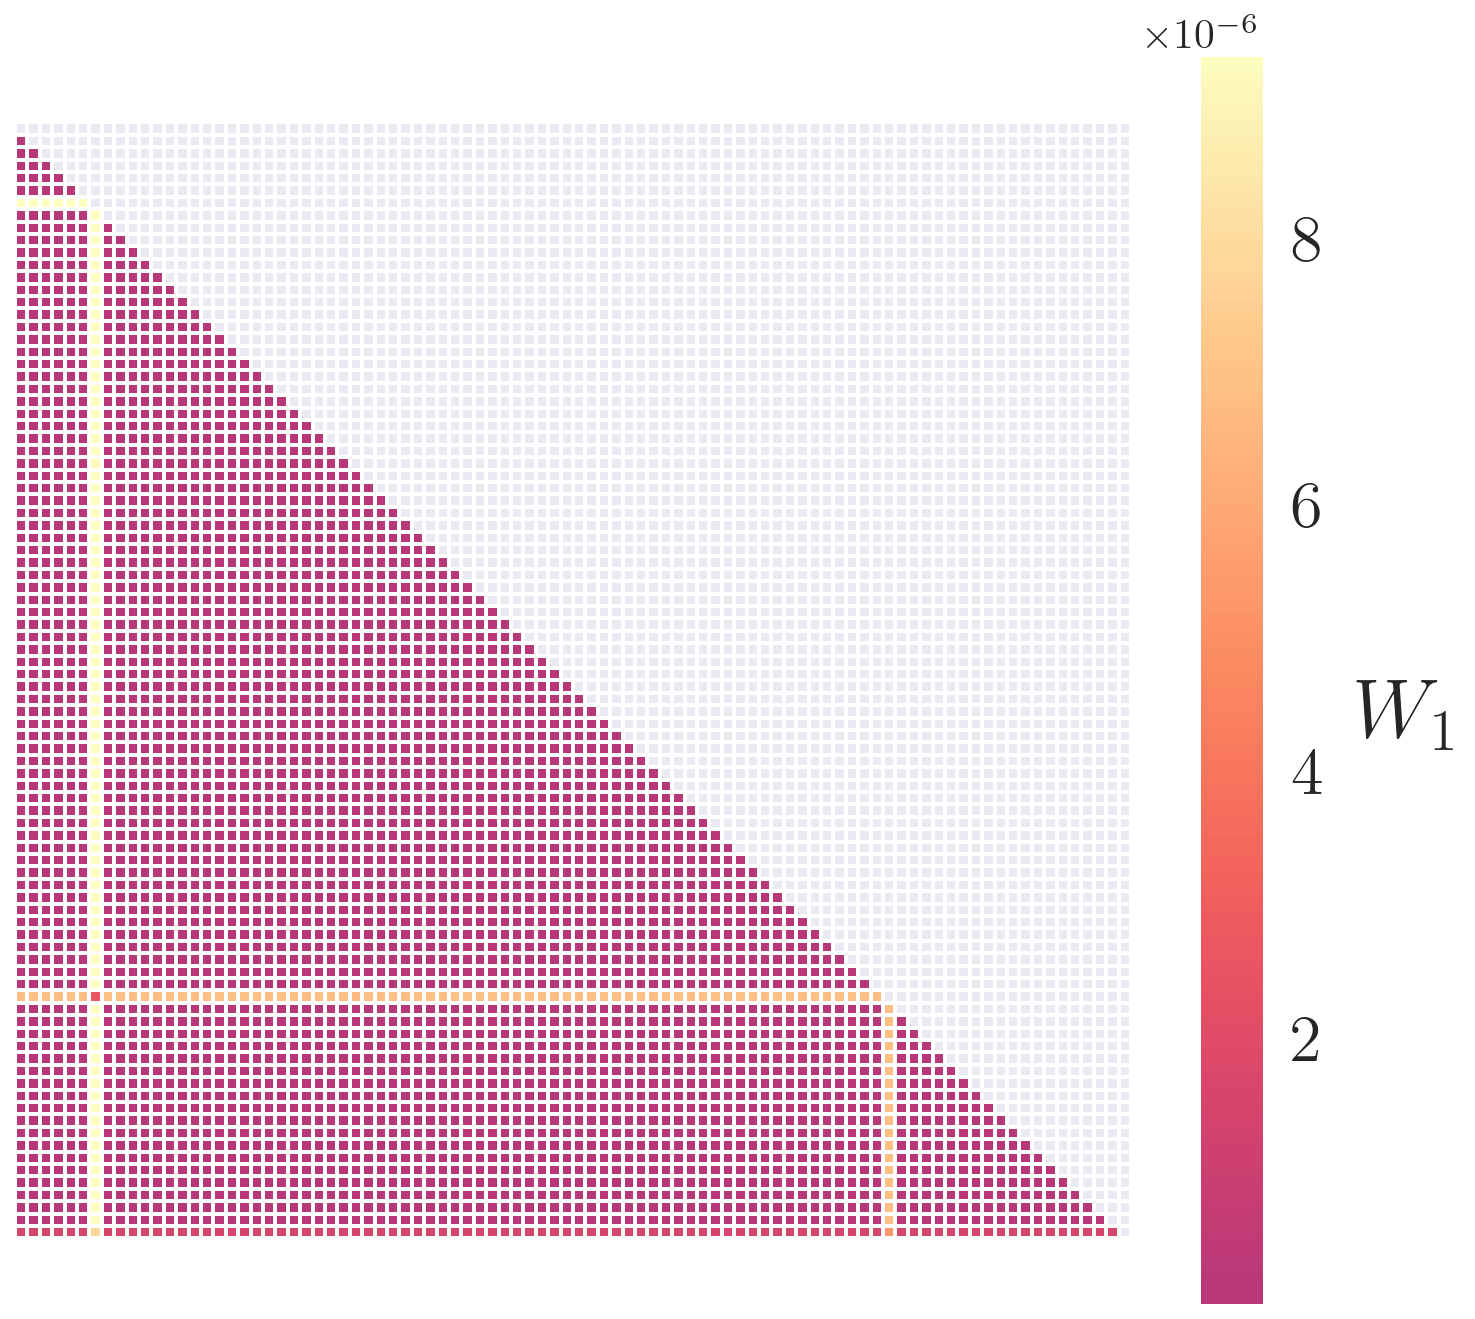
\includegraphics[width=\textwidth]{images/WD_0}
		\caption{$\Omega$}
	\end{subfigure}
	\hfill
	\begin{subfigure}[b]{0.22\textwidth}
		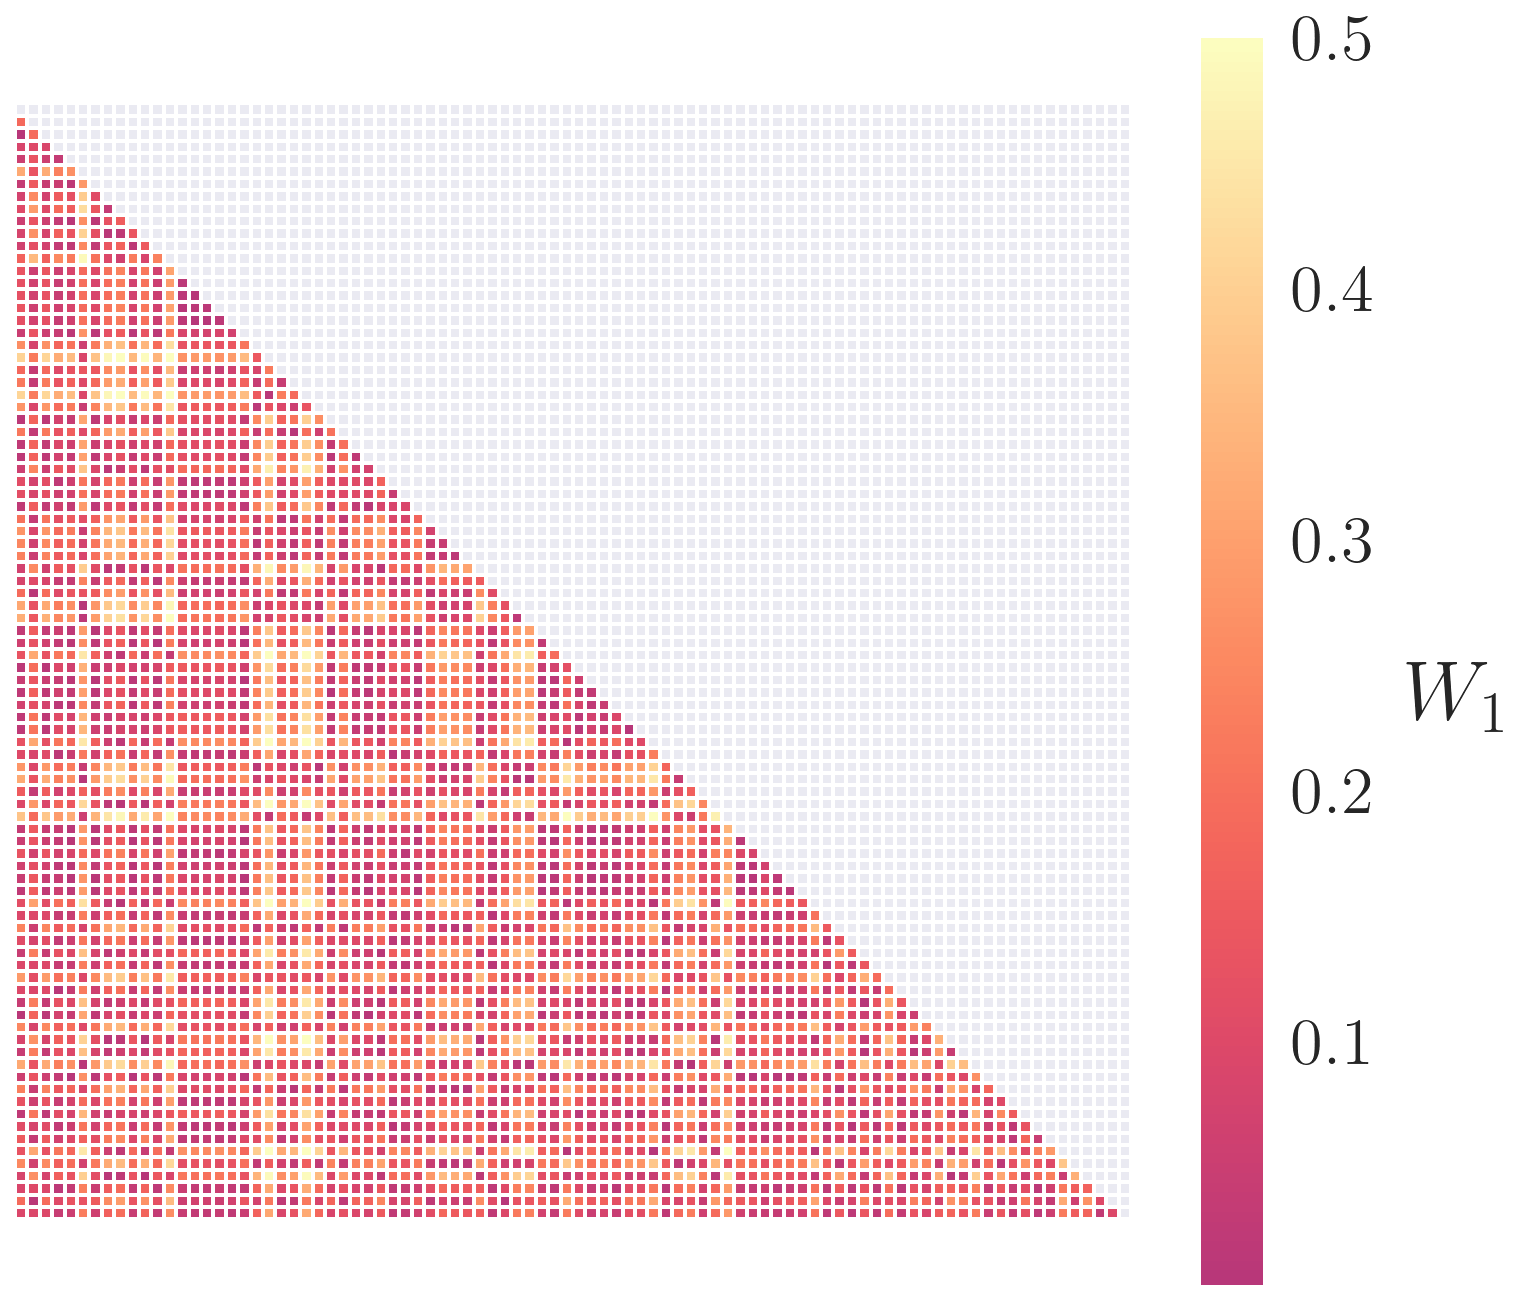
\includegraphics[width=\textwidth]{images/WD_1}
		\caption{$\Phi_0$}
	\end{subfigure}
	\hfill	
	\begin{subfigure}[b]{0.22\textwidth}
		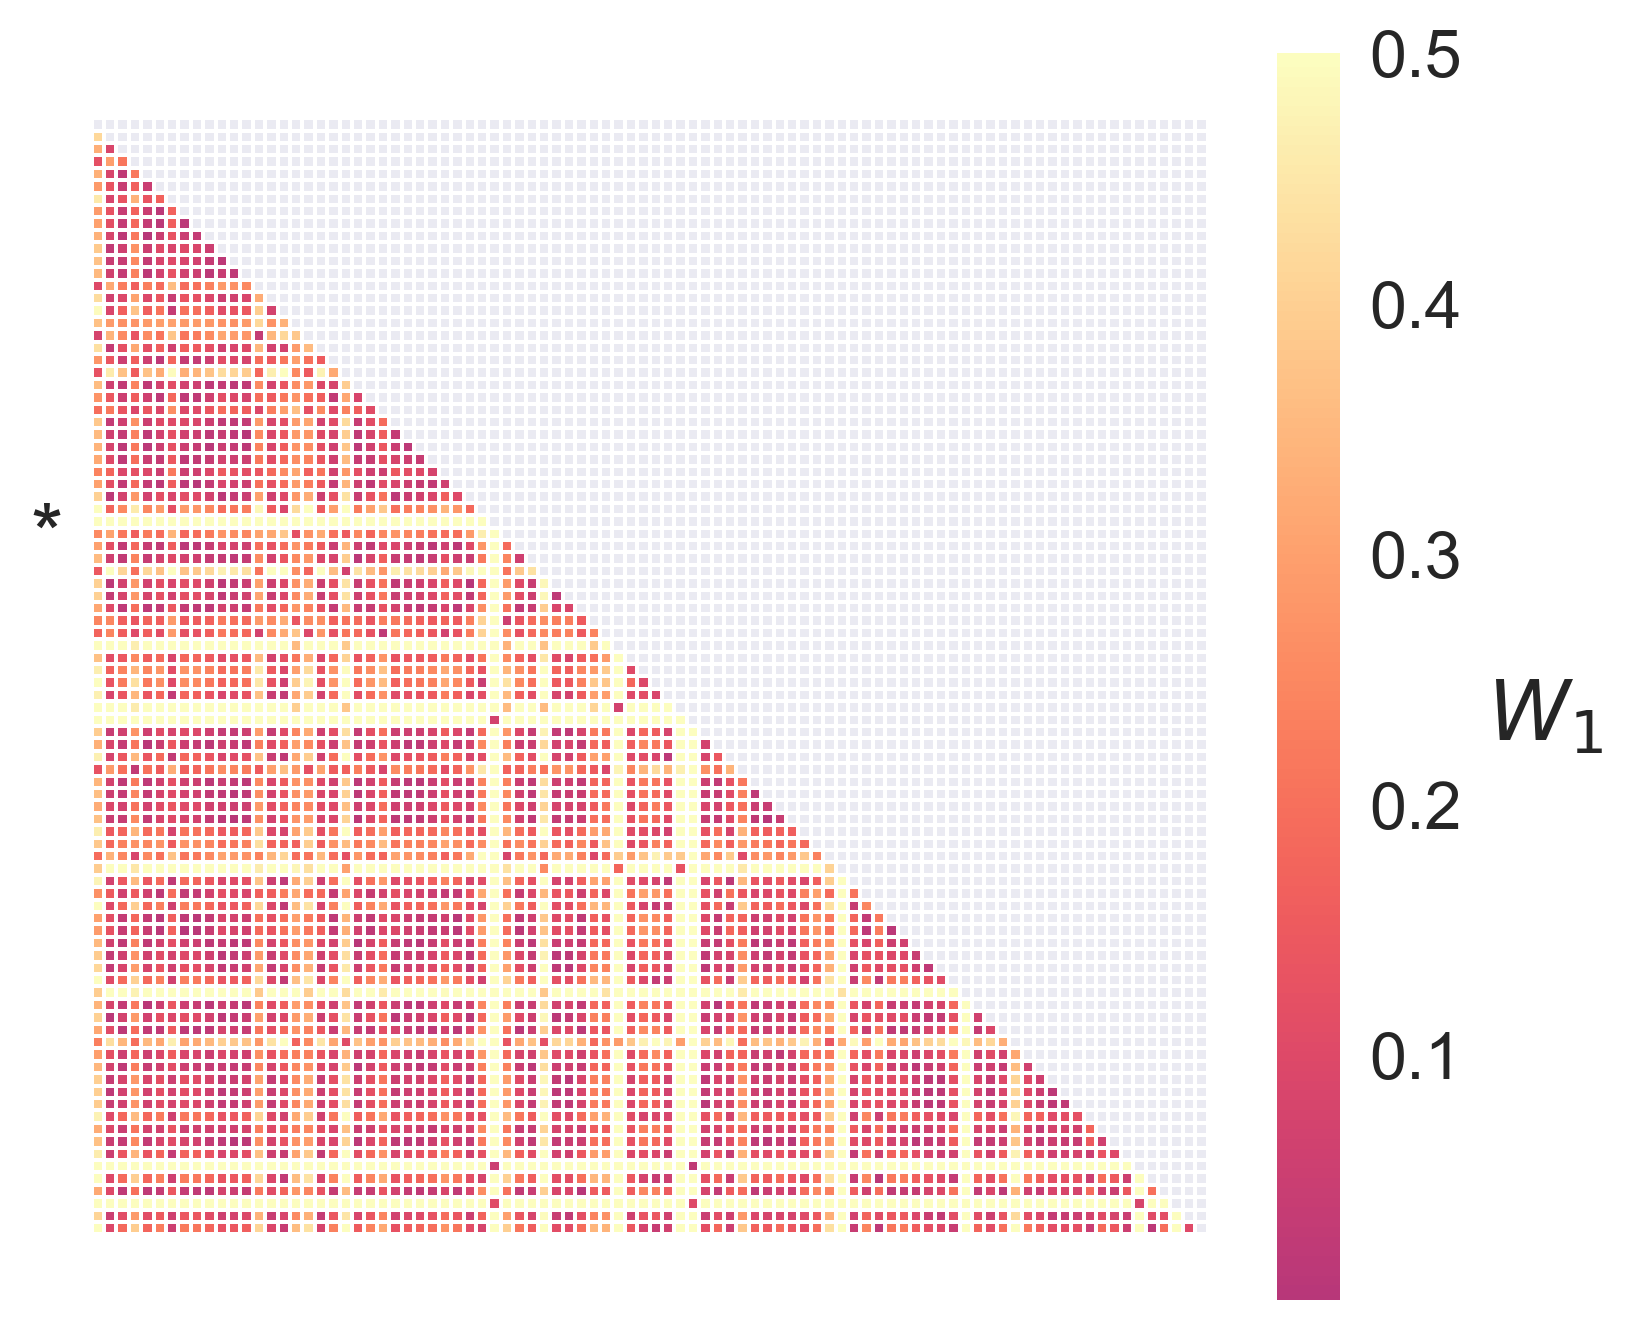
\includegraphics[width=\textwidth]{images/WD_2}
		\caption{$\psi$} \label{figWD_psi}
	\end{subfigure}
	\hfill
	\begin{subfigure}[b]{0.22\textwidth}
		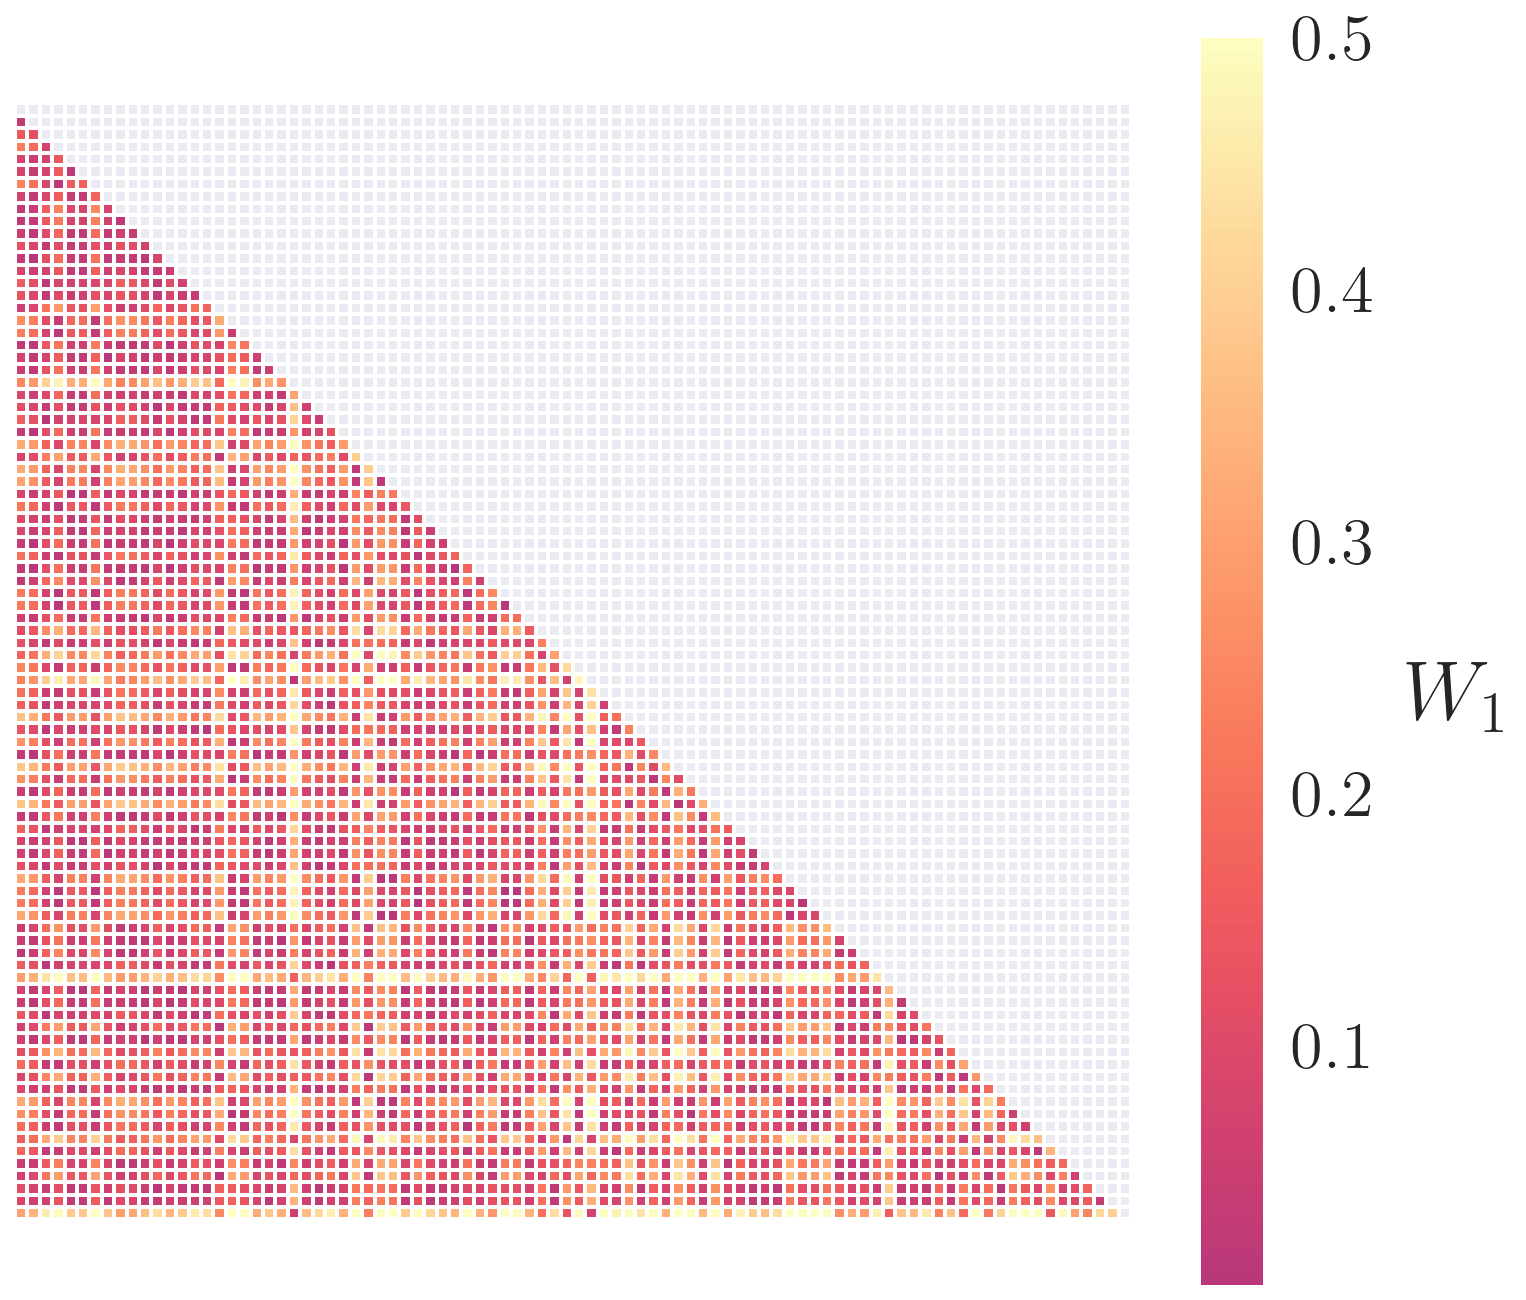
\includegraphics[width=\textwidth]{images/WD_3}
		\caption{$\iota$}
	\end{subfigure}
	\medskip
	\begin{subfigure}[b]{0.3\textwidth}
		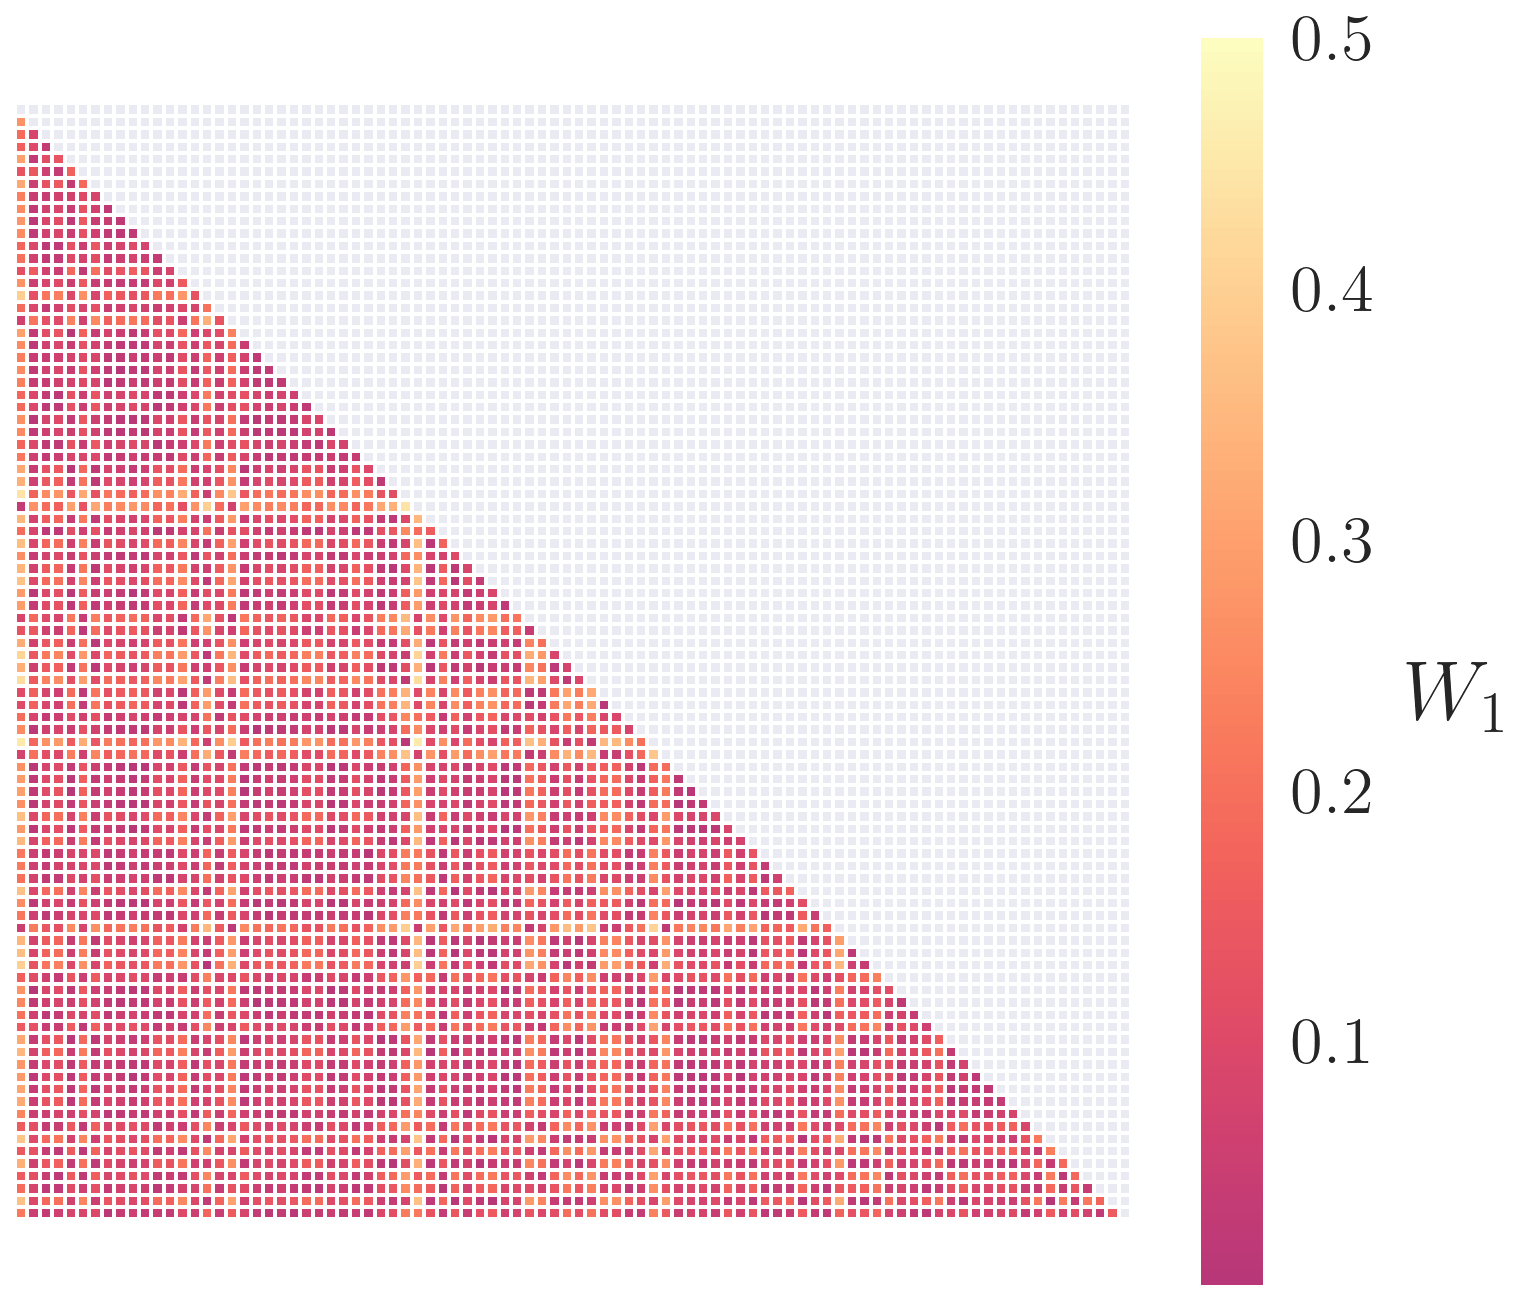
\includegraphics[width=\textwidth]{images/WD_4}
		\caption{$\delta$}
	\end{subfigure}
	\hfill	
	\begin{subfigure}[b]{0.3\textwidth}
		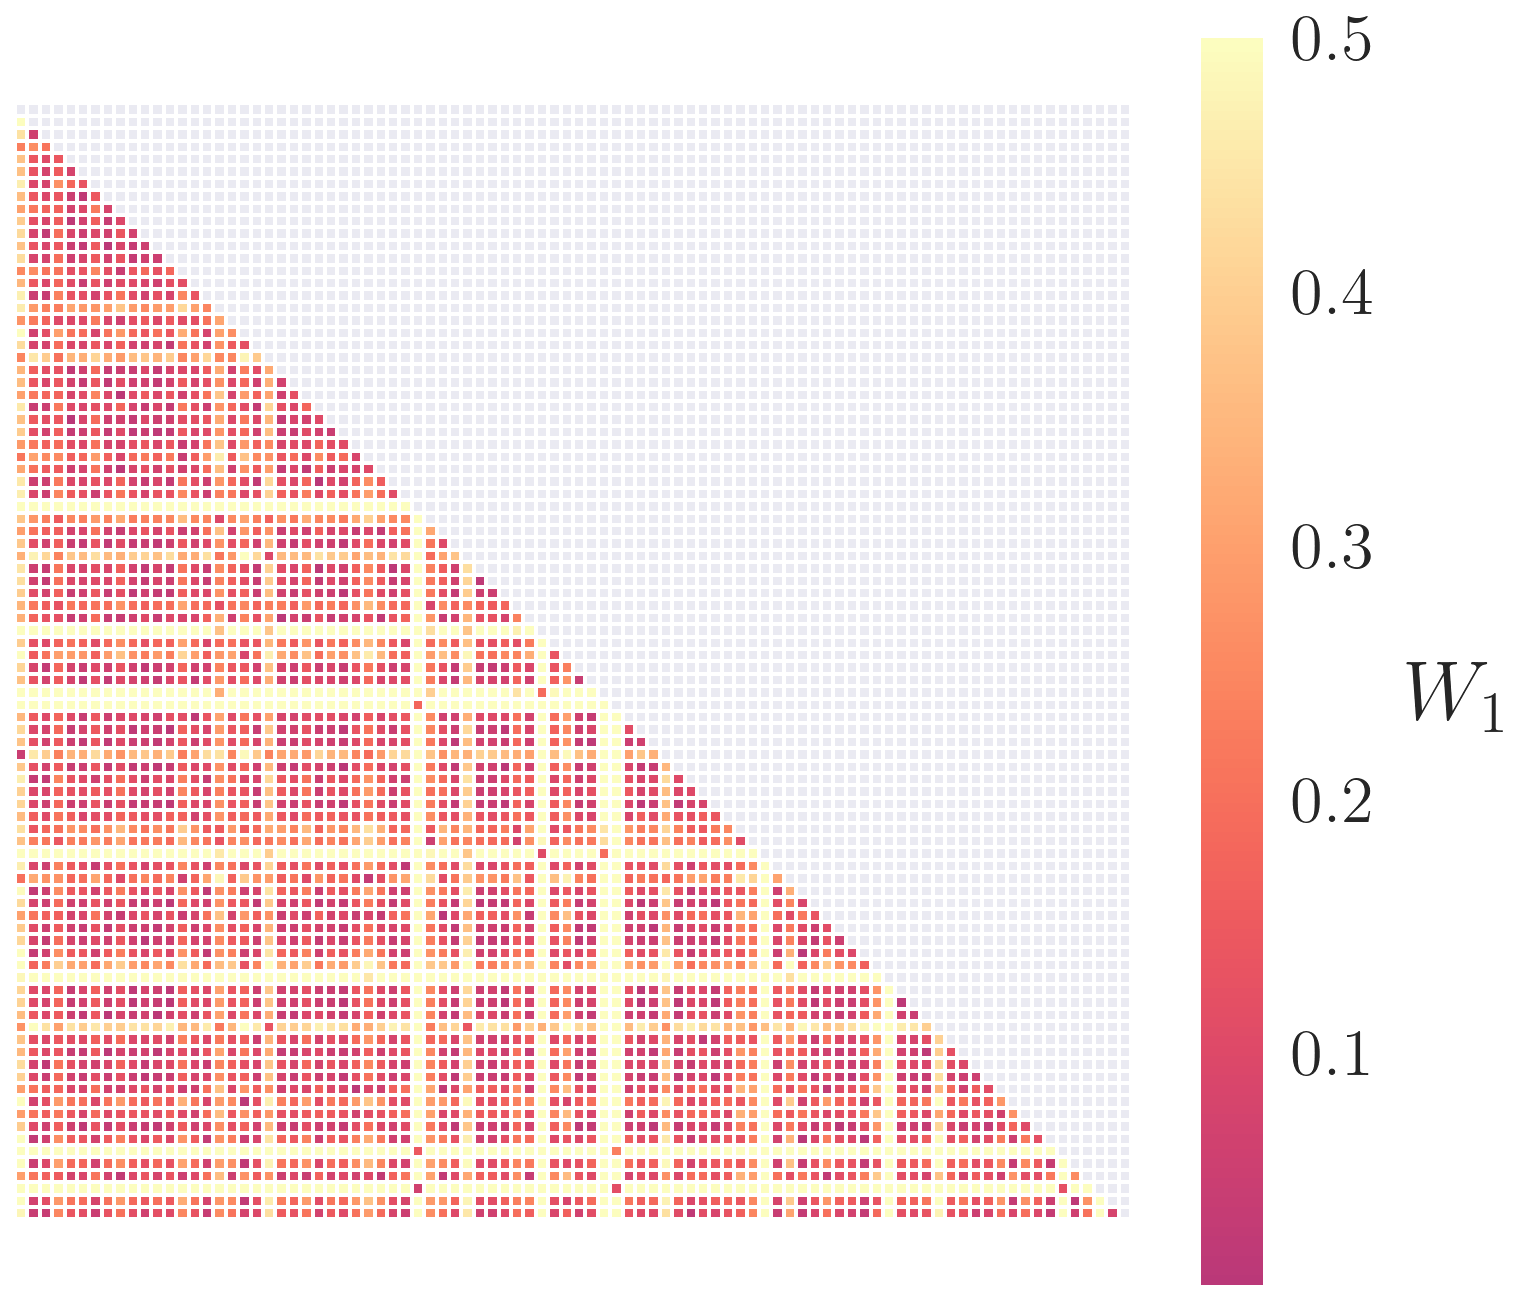
\includegraphics[width=\textwidth]{images/WD_5}
		\caption{$\alpha$}
	\end{subfigure}
	\hfill	
	\begin{subfigure}[b]{0.3\textwidth}
		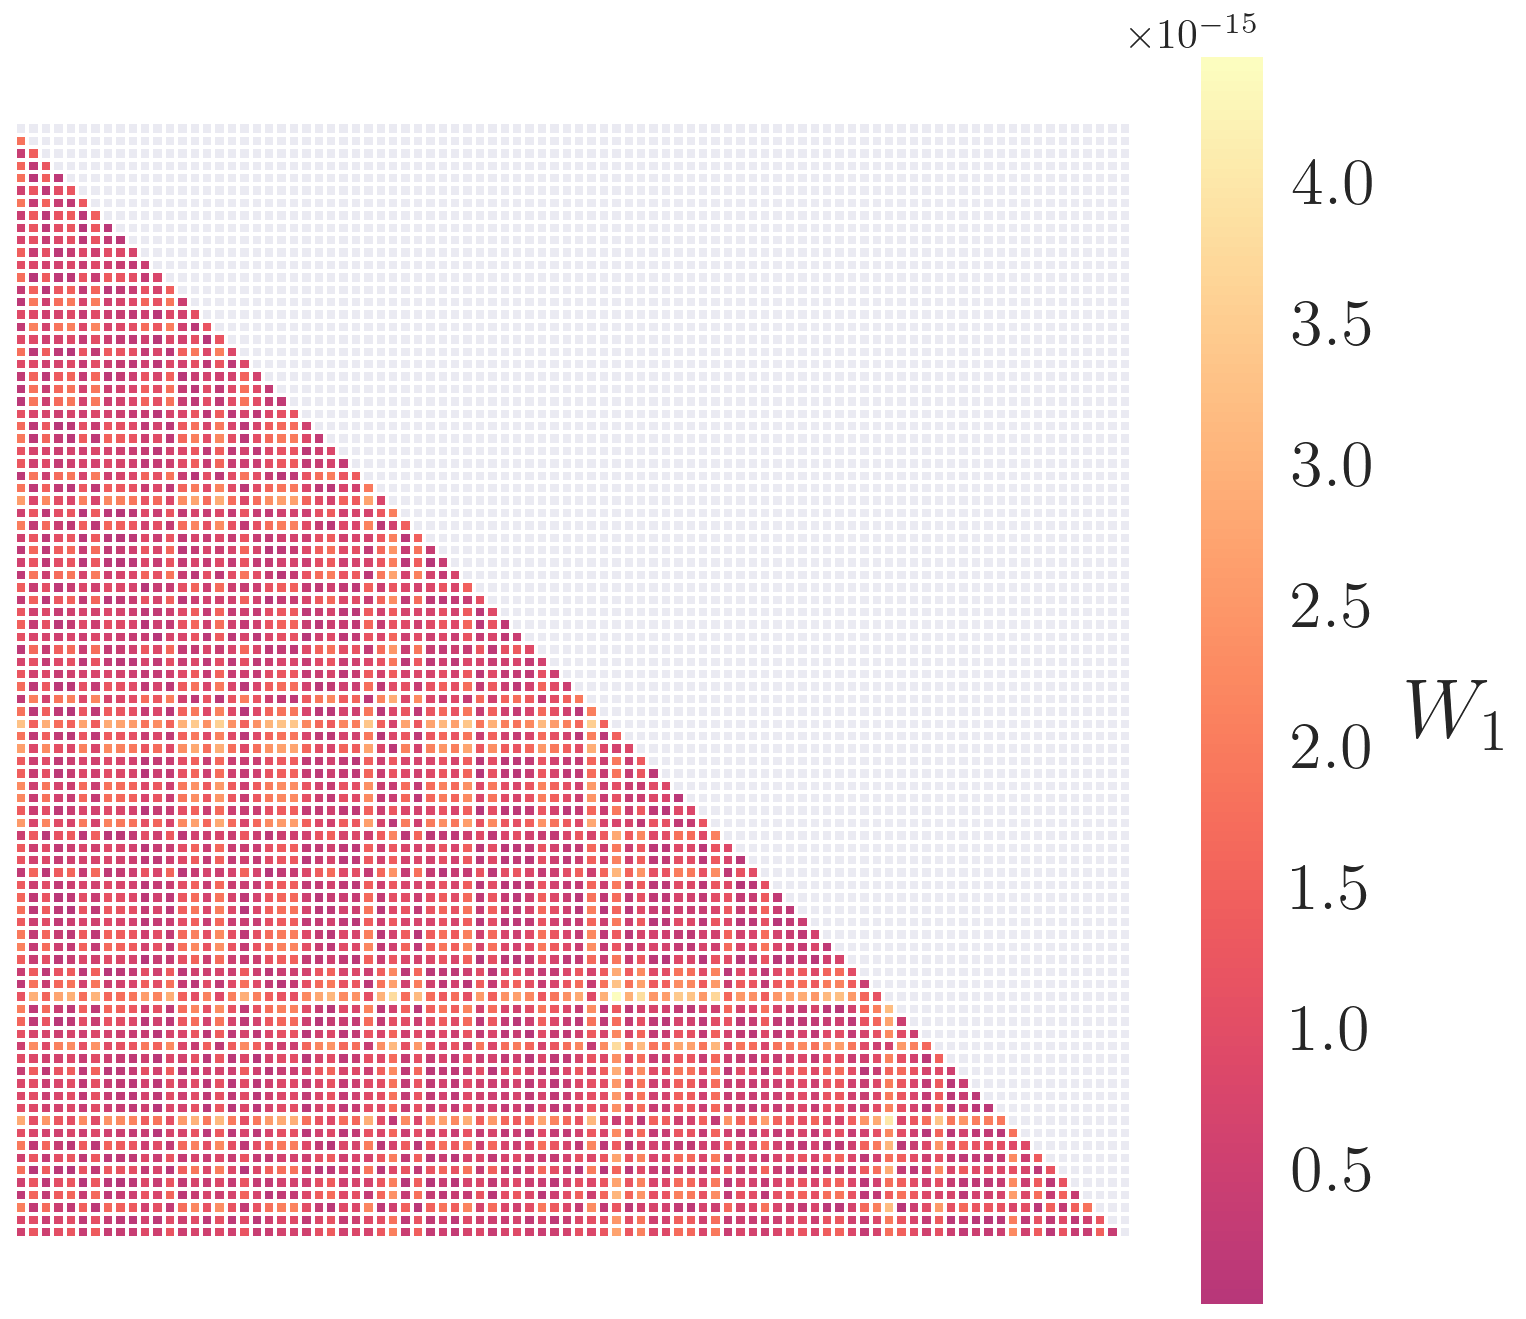
\includegraphics[width=\textwidth]{images/WD_6}
		\caption{$h$}
	\end{subfigure}
	\caption{The first moment of the Wasserstein distance, $W_1$, calculated between each pair of one-dimensional posteriors for our representative system across $10^3$ realisations, for each parameter of $\boldsymbol{\theta}_{\rm gw}$  $W_1$ provides an upper bound on the difference in expected values between any two probability distributions. $W_1$ is generally small across all parameters and all posteriors, but some posteriors converge poorly leading to large values of $W_1$. The $W_1$ values inferred for $\psi$ and $\alpha$ are strongly correlated with correlation coefficient = 0.96. An example noise realisation with particularly large pairwise $W_1$ values is labelled with an asterisk in (c) and is discussed in the text.} \label{fig:pairwise_wasserstein}
\end{figure*}
\begin{figure}
	\centering
	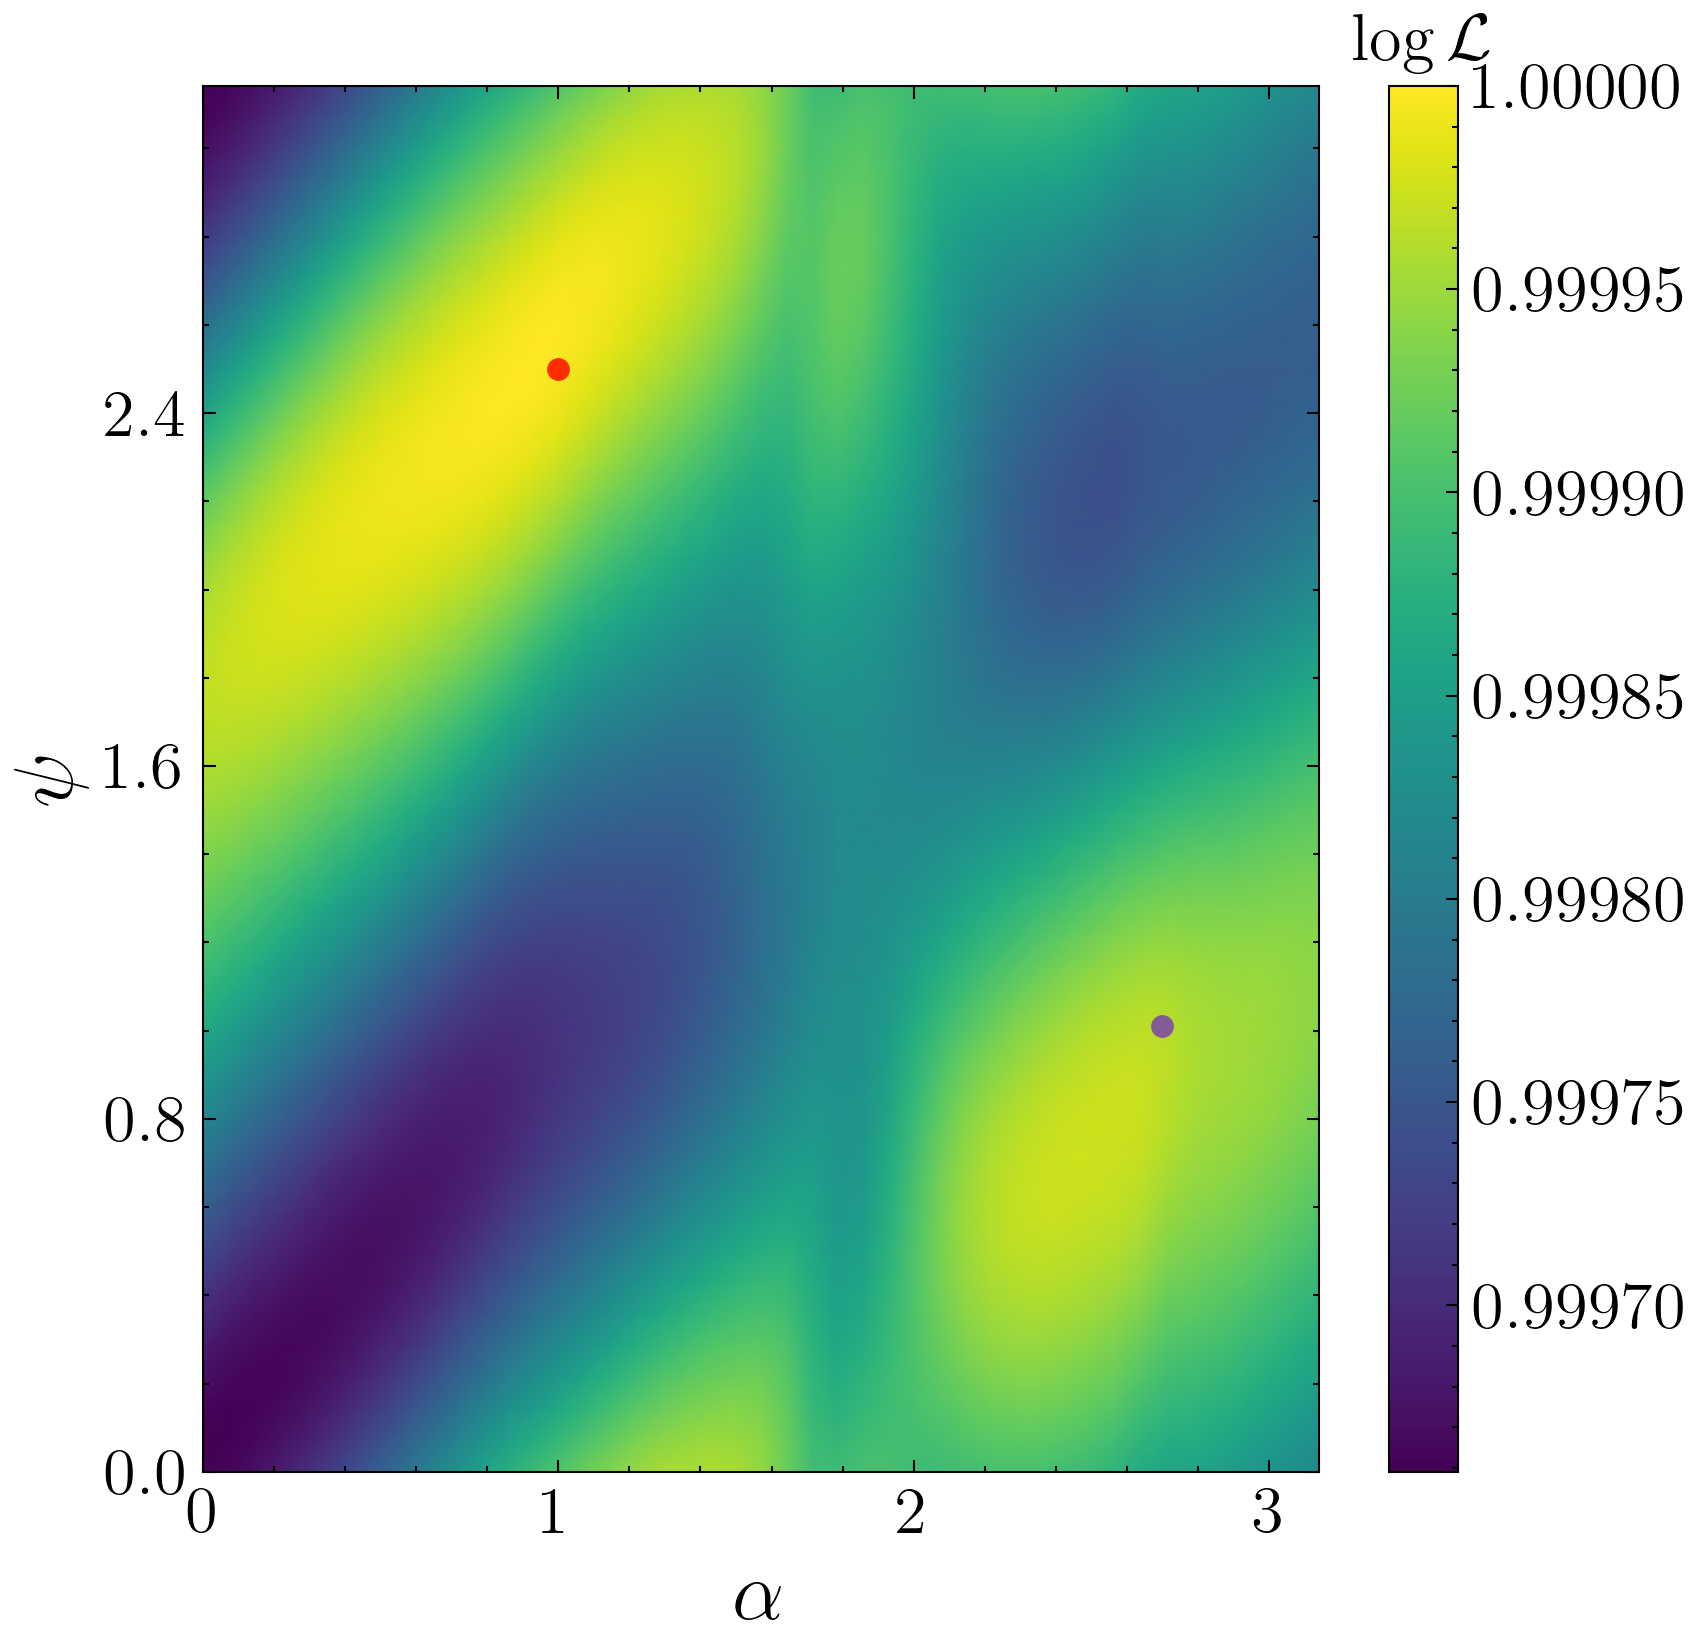
\includegraphics[width=\columnwidth]{images/likelihood_surface_alpha_psi}
	\caption{Log-likelihood, $\log \mathcal{L}$ (Equation \ref{eq:likelihood}) surface across the $\alpha-\psi$ parameter space for a single noise realisation.  The red point labels the location of the maxima, and the magenta point labels the median values of the one-dimensional posteriors inferred for a particular noise realisation of the data. The likelihood has been normalised with respect to the absolute value of the maxima. A multi-modal structure is clearly visible and for this noise realisation the nested sampler has settled in the local optima. This can be solved generally by increasing the number of live points $n_{\rm live}$.}
	\label{fig:likelihood_surface_alpha_psi}
\end{figure}







%\section{References}
%\label{sec:ref_list}





\bibliographystyle{mnras}
\bibliography{example} % if your bibtex file is called example.bib




%%%%%%%%%%%%%%%%Scratch space

%Taking a tangible example, for pulsar J0023+0923 ATNF returns a frequency $f_{\rm em}^{(n)} (t_1) \sim 327.8$ Hz with an error $\epsilon \sim 4 \times 10^{13}$ Hz. 	The prior on $f_{\rm em}^{(n)} (t_1) \sim 327.8$ for this pulsar is then Uniform$(327.8 - 4 \times 10^{10},327.8 + 4 \times 10^{10} )$


%Alternatively, one can consider instead the alternative parametrisation in terms of $h_{+}$ and $h_{\times}$. 
%
%from Equation \ref{eq:hij} the amplitude of the plane GW perturbation at a particular sky location $\boldsymbol{n}$ is a linear combination of $h_{+}$ and $h_{\times}$. 
%
%
%
%Considering a single pulsar where the only unknown parameters of the model are $h_{+}$ and $h_{\times}$, the system is clearly under-determined - we have one equation with two unknowns - and the parameters are not identifiable 
%
%



%
%
%
%
%For instance, in Figure \ref{fig:omega_likelihood} we pass different values of $\Omega$ in the range $10^{-9}$ to $10^{-5}$ Hz into the Kalman filter, whilst holding the remaining parameters constant, and plot the retuned log-likelihood as a function of $\Omega$. 
%












%
%The second is that the log-likelihood curves for $\Omega, \delta$ and $\alpha$ are much more noisy than in the Earth-terms case. Whilst clear optima exist above the noise, and whilst local to the true value the curve becomes much more smooth, this noise presents an additional challenge to typical likelihood inference techniques which perform best on smooth likelihoods with a single clear global optima. It affects these parameters in particular since Equation \eqref{eq:g_func_trig} contains a phase term $\Omega \left(1 + \boldsymbol{n}\cdot \boldsymbol{q}^{(n)} \right)  d^{(n)}$, which is essentially a combination of these 3 parameters ($ \boldsymbol{n}$ is defined by $\delta$ and $\alpha$). When calculating a likelihood we are asking "How likely is this data, given these parameters". The inclusion of the pulsar terms results in effectively 2 continuous waves with different frequencies and phase. Perturbing e.g. $\alpha$ influences wave 1 in some non-liner way and wave 2 in some different non linear way. Whether this new set of parameters makes the data more likely depends on the particular combination of those two waves. \textcolor{red}{TK: this explanation of why these parameters is clunky because it is not properly clear to myself. Think in terms of $g(\theta)$ and $g(\hat{\theta})$}. 






%
%. In turn, each posterior distribution has a median value. We plot the distribution of these medians over the 1000 noise realisations for each parameter of $\boldsymbol{\theta}_{\rm gw}$ in Figure \ref{fig:median_distriubutins}. For each of these distributions we can also calculate the median value (i.e. the median of the medians) and compare it with the true injection value. This is shown by the red and orange dashed lines respectively in the Figure. Analogous to the results we saw in Figure \ref{fig:corner_plot_2}, the distributions of the median values of the parameters $\Omega, \Phi_0, \psi, \delta$ and $\alpha$ are very narrow, with a generally small discrepancy between the inferred value and the injected value. Conversely, the distributions for $\iota$ and $h_0$ are much broader and exhibit a bias of $\sim 0.18$ radians and $0.17 \times 10^{-12}$ respectively. This agrees with the results we discussed for the 9 noise realisations in Figure \ref{fig:corner_plot_2} where a bias in $\iota$ and $h_0$ was also observed. In addition to  $\iota$ and $h_0$  exhibiting a strong bias, the parameters $\psi$ and $\alpha$ also exhibit a small bias of magnitude $\sim 0.1$ and $\sim 0.04$ radians respectively. This bias is again a result of dropping the pulsar terms from the measurement equation and will be discussed in . 












%%%%%%%%%%%%%%%%%%%%%%%%%%%%%%%%%%%%%%%%%%%%%%%%%%


% Don't change these lines
\bsp	% typesetting comment
\label{lastpage}
\end{document}

% End of mnras_guide.tex
